
\chapter{Vector Calculus}

\section*{Introduction}

Every river has a current. Every atmosphere has wind. Every charged body is immersed in an electromagnetic field. At every point in space, there is a vector---a direction and a magnitude---telling a particle which way to go and how hard it will be pushed. These are \textit{vector fields}, and they are everywhere. This chapter develops the calculus to work with them.\\ \\
\noindent We begin with \textit{line integrals}, which compute work done by a force along a curved path, and \textit{surface integrals}, which measure the flux of a field through a surface. Then comes the crown jewel: three theorems---\textbf{Green's}, \textbf{Stokes'}, and the \textbf{Divergence Theorem}---that reveal these integrals are not independent at all. Each says the same profound thing at a different dimensional level: \textit{what happens on the boundary is completely determined by what happens inside.}\\ \\
\noindent This is the culmination of everything we have built---limits, derivatives, integrals, vectors, multiple integrals---woven into a single framework. The Fundamental Theorem of Calculus said differentiation and integration are inverse operations on an interval. Green's, Stokes', and the Divergence Theorem say the same thing for curves, surfaces, and volumes. These results are the foundation of Maxwell's equations, the Navier-Stokes equations, and the conservation laws that govern every physical theory. They are, in the truest sense, where calculus grows up.

\newpage 





\lecture{Vector Fields}  \index{Vector Fields}

\noindent Our journey through multivariable calculus has led us through scalar functions, where we mapped points in space to single numerical values. For instance, we could assign a temperature to each point in a room, or a pressure value to each point in the atmosphere. But many physical quantities we encounter can't be fully described by just a single number—they need both a magnitude and a direction. \\

\noindent Think about the wind blowing across a vast plain. At each point in space, the wind has both a speed (magnitude) and a direction. Or imagine iron filings scattered near a magnet—at each point, there's a magnetic force acting with a specific strength and orientation. These are examples where we need to assign not just a number, but a vector to each point in space.

\begin{figure}[H]
\centering
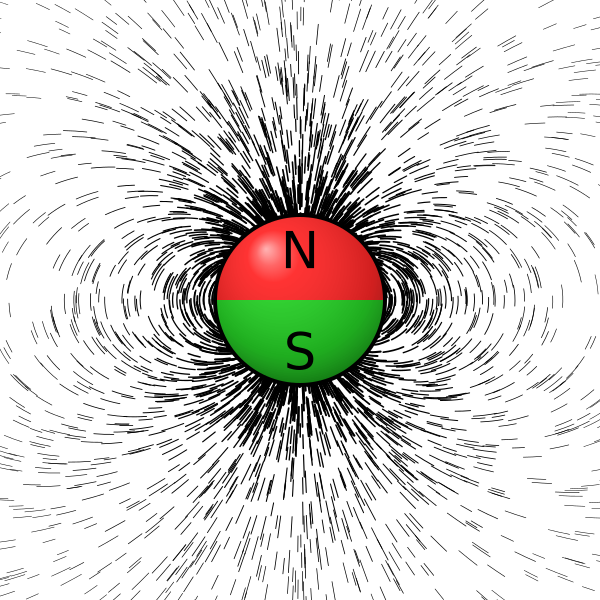
\includegraphics[width=0.4\textwidth]{chapters/chp5_pics/magnet.png}
\caption{\textit{A magnet pulling iron filings is a physical representation of a vector field. Each point around the magnet has a magnitude of force and direction emanating from the magnet}}
\label{fig:magnet}
\end{figure}

\noindent Let's build this idea carefully. Start by imagining a single point $(x_0,y_0)$ in the plane. At this point, we want to attach a vector—perhaps representing wind velocity. This vector will have both an $x$-component and a $y$-component, which we might call $P(x_0,y_0)$ and $Q(x_0,y_0)$ respectively. The vector at this point would then be:
\[
\mathbf{v}_{(x_0,y_0)} = P(x_0,y_0)\mathbf{i} + Q(x_0,y_0)\mathbf{j}
\]

\noindent Now imagine doing this for every point in the plane. As we move to different points $(x,y)$, both components of our vector might change—the wind might blow in different directions and with different speeds at different locations. We're no longer just looking at a single vector, but at a function that assigns a vector to every point. This is the essence of a vector field.

\subsection*{Definition and Basic Properties}

\noindent Formally, a \textbf{vector field} $\mathbf{F}$ in $\mathbb{R}^n$ is a function that assigns to each point $\mathbf{p}$ in its domain a vector $\mathbf{F}(\mathbf{p})$. Just as scalar fields mapped points to numbers, vector fields map points to vectors. In two dimensions, this means associating each point $(x,y)$ with a two-dimensional vector:
\[
\mathbf{F}(x,y) = P(x,y)\mathbf{i} + Q(x,y)\mathbf{j}
\]

\noindent Here, $P(x,y)$ gives the $x$-component of the vector at any point $(x,y)$, while $Q(x,y)$ gives the $y$-component. To understand how this works in practice, let's break down the process of evaluating a vector field at specific points. \\

\noindent Consider a simple vector field $\mathbf{F}(x,y) = x\mathbf{i} + y\mathbf{j}$. Here, $P(x,y) = x$ and $Q(x,y) = y$. To plot vectors in this field:

\begin{center}
\begin{tabular}{|c|c||c|c|c|}
\hline
$x$ & $y$ & Vector Tail at & $P(x,y)$ & $Q(x,y)$ \\
\hline
1 & 1 & (1,1) & 1 & 1 \\
2 & 1 & (2,1) & 2 & 1 \\
1 & 2 & (1,2) & 1 & 2 \\
-1 & 1 & (-1,1) & -1 & 1 \\
\hline
\end{tabular}
\end{center}

\noindent At each point $(x,y)$, we:
\begin{enumerate}
   \item Place the tail of our vector at the point $(x,y)$
   \item Move $P(x,y)$ units in the $\mathbf{i}$ direction
   \item Move $Q(x,y)$ units in the $\mathbf{j}$ direction
\end{enumerate}

\noindent For example, at the point $(2,1)$, we place our vector tail at $(2,1)$, then move 2 units in the $\mathbf{i}$ direction and 1 unit in the $\mathbf{j}$ direction, resulting in a vector pointing to $(4,2)$. \\

\noindent The idea extends naturally to three dimensions. At each point $(x,y,z)$ in space, we now need three components to specify a vector:
\[
\mathbf{F}(x,y,z) = P(x,y,z)\mathbf{i} + Q(x,y,z)\mathbf{j} + R(x,y,z)\mathbf{k}
\]

\noindent For instance, in the three-dimensional vector field $\mathbf{F}(x,y,z) = z\mathbf{i} + x\mathbf{j} + y\mathbf{k}$:

\begin{center}
\begin{tabular}{|c|c|c||c|c|c|}
\hline
$x$ & $y$ & $z$ & $P(x,y,z)$ & $Q(x,y,z)$ & $R(x,y,z)$ \\
\hline
1 & 2 & 3 & 3 & 1 & 2 \\
2 & 1 & 0 & 0 & 2 & 1 \\
-1 & 0 & 2 & 2 & -1 & 0 \\
\hline
\end{tabular}
\end{center}

\noindent At each point $(x,y,z)$, we:
\begin{enumerate}
   \item Place the tail of our vector at the point $(x,y,z)$
   \item Move $P(x,y,z)$ units in the $\mathbf{i}$ direction
   \item Move $Q(x,y,z)$ units in the $\mathbf{j}$ direction
   \item Move $R(x,y,z)$ units in the $\mathbf{k}$ direction
\end{enumerate}

\noindent For example, at the point $(1,2,3)$, the vector starts at $(1,2,3)$ and has components $\langle 3,1,2 \rangle$, meaning it extends 3 units in the $x$-direction, 1 unit in the $y$-direction, and 2 units in the $z$-direction. \\

\noindent The functions $P$, $Q$, and $R$ are called the \textbf{component functions} of the vector field. Each represents the magnitude of the field's projection onto one of the coordinate axes. Just as coordinates tell us where we are in space, these component functions tell us what vector we'll find when we get there. \\

\noindent Just as we studied continuity and differentiability for scalar functions—concepts that told us how ``smoothly" the function varied as we moved around—these ideas extend naturally to vector fields. A vector field is continuous if all its component functions are continuous, meaning the vectors change smoothly as we move from point to point. Similarly, a vector field is differentiable if all its component functions are differentiable, allowing us to analyze rates of change in the field's behavior.


\subsection*{Visualizing Vector Fields}

\noindent After understanding how to evaluate vector fields at individual points, our next step is visualizing them across regions of space. When we plot a vector field, we draw arrows at carefully chosen points to represent the field's behavior. Each arrow has two key properties:
\begin{itemize}
   \item The direction of the arrow shows where the vector field points at that location
   \item The length (or magnitude) of the arrow indicates the vector's strength at that point
\end{itemize}

\noindent Let's develop this systematically. Consider the vector field $\mathbf{F}(x,y) = -y\mathbf{i} + x\mathbf{j}$. To begin visualizing this field, we'll evaluate it at several points using a grid:

\begin{center}
\begin{tabular}{|c|c||c|c|c|}
\hline
$x$ & $y$ & Vector Tail at & $P(x,y) = -y$ & $Q(x,y) = x$ \\
\hline
1 & 1 & (1,1) & -1 & 1 \\
1 & -1 & (1,-1) & 1 & 1 \\
-1 & -1 & (-1,-1) & 1 & -1 \\
-1 & 1 & (-1,1) & -1 & -1 \\
\hline
\end{tabular}
\end{center}

\noindent For each point in our table, we plot a straight arrow by:
\begin{enumerate}
   \item Starting at the tail point $(x,y)$
   \item Drawing a straight line in the direction $\langle P(x,y), Q(x,y) \rangle$
   \item Optionally normalize it by dividing by $\sqrt{P(x,y)^2 + Q(x,y)^2}$
\end{enumerate}

\noindent It's crucial to note that regardless of the vector field, each arrow we draw is always straight—even if the overall pattern suggests rotation or curvature. Each arrow represents the instantaneous direction of the field at a single point. \\

\noindent For example, here's how we would visualize this field:

\begin{center}
\begin{tikzpicture}[scale=1.5]
% Draw axes
\draw[->] (-2,0) -- (2,0) node[right] {$x$};
\draw[->] (0,-2) -- (0,2) node[above] {$y$};

% Draw vectors at diagonal points
\draw[blue,thick,->] (1,1) -- (0,2);
\draw[blue,thick,->] (1,-1) -- (2,0);
\draw[blue,thick,->] (-1,-1) -- (0,-2);
\draw[blue,thick,->] (-1,1) -- (-2,0);

% Label points
\fill (1,1) circle (1pt);
\fill (1,-1) circle (1pt);
\fill (-1,-1) circle (1pt);
\fill (-1,1) circle (1pt);

% Add point labels
\node[above right] at (1,1) {$(1,1)$};
\node[below right] at (1,-1) {$(1,-1)$};
\node[below left] at (-1,-1) {$(-1,-1)$};
\node[above left] at (-1,1) {$(-1,1)$};
\end{tikzpicture}
\end{center}

\noindent Notice how even with just these four points, we can begin to see the rotational pattern emerging in the field. Together the arrows suggest a counterclockwise circulation around the origin. Here's an example of a complete field generated systematically for $\mathbf{F}(x,y) = -y\mathbf{i} + x\mathbf{j}$:

\begin{figure}[H]
\centering
   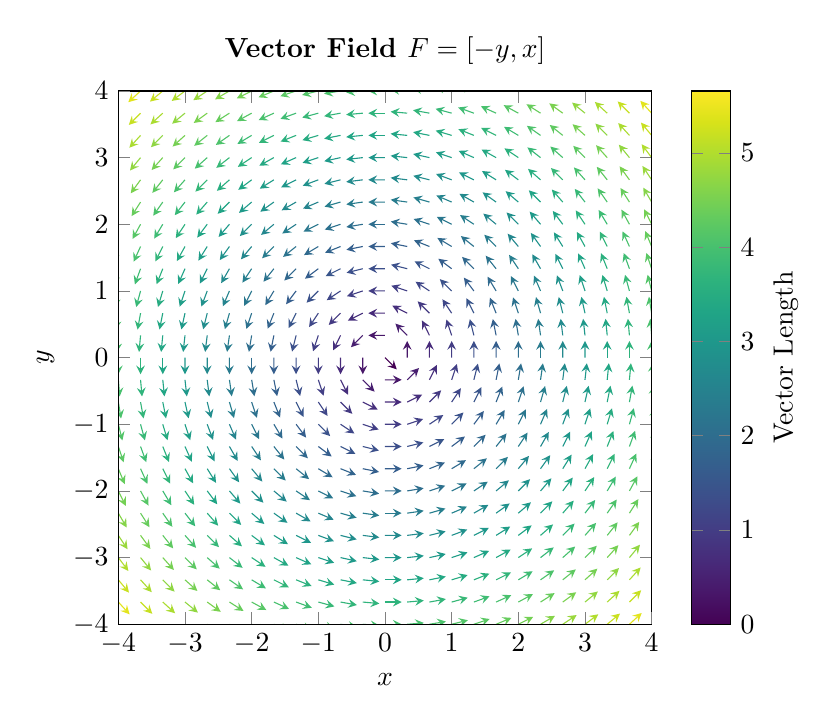
\begin{tikzpicture}
       \begin{axis}[
           xmin = -4, xmax = 4,
           ymin = -4, ymax = 4,
           zmin = 0, zmax = 1,
           axis equal image,
           xtick distance = 1,
           ytick distance = 1,
           view = {0}{90},
           scale = 1.25,
           title = {\bf Vector Field $F = [-y,x]$},
           height=7cm,
           xlabel = {$x$},
           ylabel = {$y$},
           colormap/viridis,
           colorbar,
           colorbar style = {
               ylabel = {Vector Length}
           }
       ]
           \addplot3[
               point meta = {sqrt(x^2+y^2)},
               quiver = {
                   u = {-y/sqrt(x^2+y^2)},
                   v = {x/sqrt(x^2+y^2)},
                   scale arrows = 0.25,
               },
               quiver/colored = {mapped color},
               -stealth,
               domain = -4:4,
               domain y = -4:4,
           ] {0};
       \end{axis}
   \end{tikzpicture}
\caption{\textit{The circular pattern emerges from the collective behavior of many straight arrows, each showing the instantaneous direction at its starting point. This is analogous to how the tangent line approximates a curve at a single point—each vector arrow shows the field's direction at just one point in space.}}
\end{figure}


\noindent When we plot many more points, patterns emerge in the vector field. These patterns help us identify important features:

\begin{itemize}
   \item \textbf{Sources:} Points where vectors emanate outward, like water springing from a fountain. For example, in the field $\mathbf{F}(x,y) = x\mathbf{i} + y\mathbf{j}$, the origin is a source:
   
   \begin{figure}[H]
   \centering
   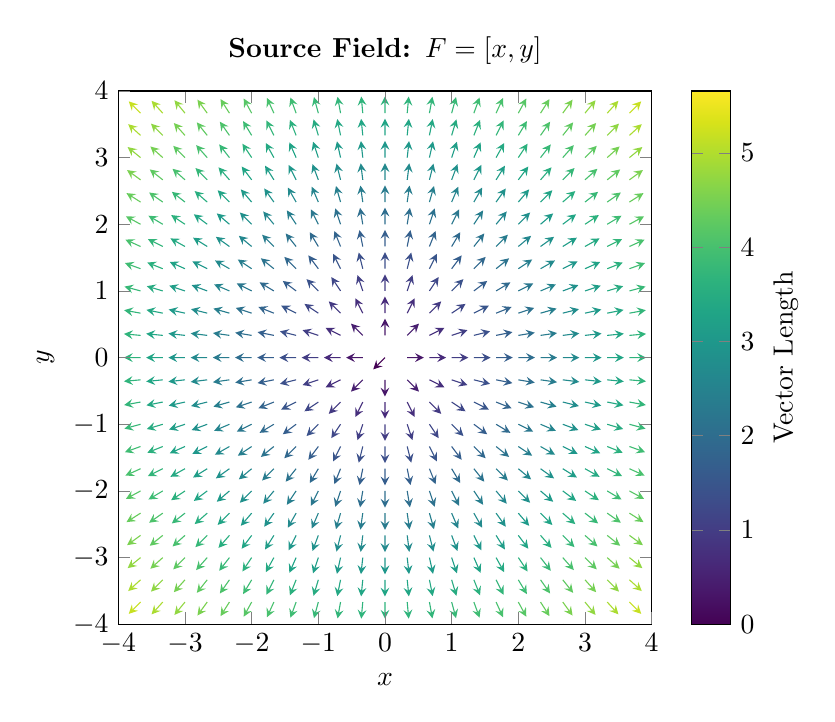
\begin{tikzpicture}
   \begin{axis}[
       xmin = -4, xmax = 4,
       ymin = -4, ymax = 4,
       zmin = 0, zmax = 1,
       axis equal image,
       xtick distance = 1,
       ytick distance = 1,
       view = {0}{90},
       scale = 1.25,
       title = {\bf Source Field: $F = [x,y]$},
       height=7cm,
       xlabel = {$x$},
       ylabel = {$y$},
       colormap/viridis,
       colorbar,
       colorbar style = {
           ylabel = {Vector Length}
       }
   ]
       \addplot3[
           point meta = {sqrt(x^2+y^2)},
           quiver = {
               u = {x/sqrt(x^2+y^2)},
               v = {y/sqrt(x^2+y^2)},
               scale arrows = 0.25,
           },
           quiver/colored = {mapped color},
           -stealth,
           domain = -4:4,
           domain y = -4:4,
       ] {0};
   \end{axis}
   \end{tikzpicture}
   \end{figure}

   \item \textbf{Sinks:} Points where vectors converge inward, like water draining from a bathtub. The field $\mathbf{F}(x,y) = -x\mathbf{i} - y\mathbf{j}$ has a sink at the origin:
   
   \begin{figure}[H]
   \centering
   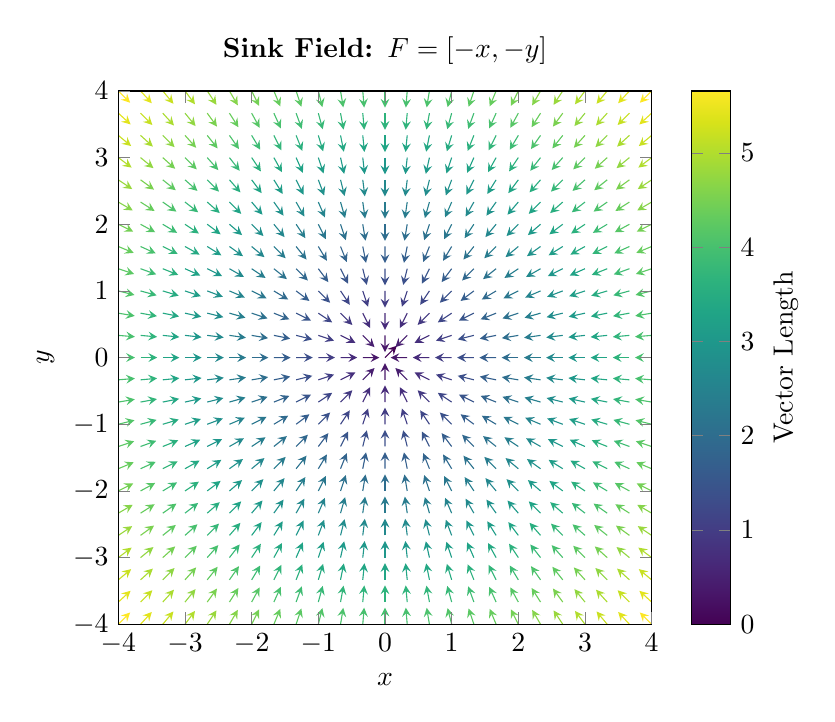
\begin{tikzpicture}
   \begin{axis}[
       xmin = -4, xmax = 4,
       ymin = -4, ymax = 4,
       zmin = 0, zmax = 1,
       axis equal image,
       xtick distance = 1,
       ytick distance = 1,
       view = {0}{90},
       scale = 1.25,
       title = {\bf Sink Field: $F = [-x,-y]$},
       height=7cm,
       xlabel = {$x$},
       ylabel = {$y$},
       colormap/viridis,
       colorbar,
       colorbar style = {
           ylabel = {Vector Length}
       }
   ]
       \addplot3[
           point meta = {sqrt(x^2+y^2)},
           quiver = {
               u = {-x/sqrt(x^2+y^2)},
               v = {-y/sqrt(x^2+y^2)},
               scale arrows = 0.25,
           },
           quiver/colored = {mapped color},
           -stealth,
           domain = -4:4,
           domain y = -4:4,
       ] {0};
   \end{axis}
   \end{tikzpicture}
   \end{figure}

   \item \textbf{Circulation:} Regions where vectors suggest rotational motion, like our example field $\mathbf{F}(x,y) = -y\mathbf{i} + x\mathbf{j}$. Remember though—each individual arrow is still straight!
   
   \begin{figure}[H]
   \centering
   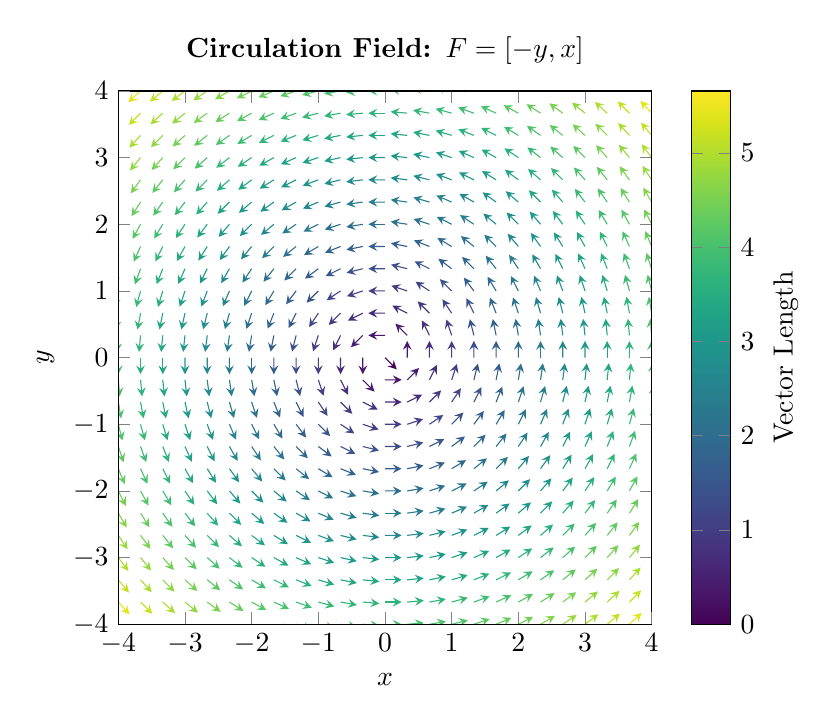
\begin{tikzpicture}
   \begin{axis}[
       xmin = -4, xmax = 4,
       ymin = -4, ymax = 4,
       zmin = 0, zmax = 1,
       axis equal image,
       xtick distance = 1,
       ytick distance = 1,
       view = {0}{90},
       scale = 1.25,
       title = {\bf Circulation Field: $F = [-y,x]$},
       height=7cm,
       xlabel = {$x$},
       ylabel = {$y$},
       colormap/viridis,
       colorbar,
       colorbar style = {
           ylabel = {Vector Length}
       }
   ]
       \addplot3[
           point meta = {sqrt(x^2+y^2)},
           quiver = {
               u = {-y/sqrt(x^2+y^2)},
               v = {x/sqrt(x^2+y^2)},
               scale arrows = 0.25,
           },
           quiver/colored = {mapped color},
           -stealth,
           domain = -4:4,
           domain y = -4:4,
       ] {0};
   \end{axis}
   \end{tikzpicture}
   \end{figure}

   \item \textbf{Saddle Points:} Points exhibiting both attractive and repulsive behavior, like the origin in $\mathbf{F}(x,y) = x\mathbf{i} - y\mathbf{j}$:
   
   \begin{figure}[H]
   \centering
   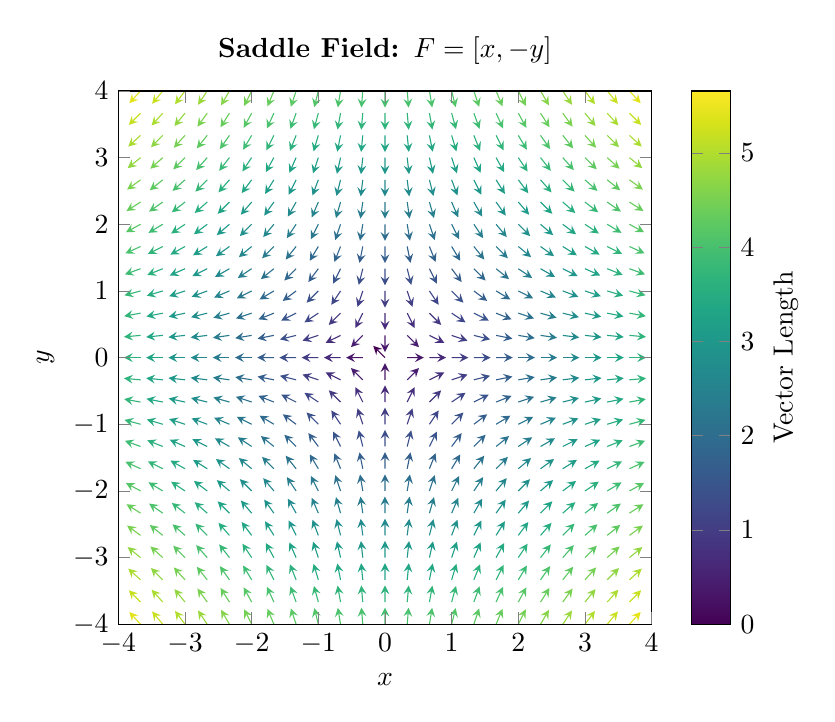
\begin{tikzpicture}
   \begin{axis}[
       xmin = -4, xmax = 4,
       ymin = -4, ymax = 4,
       zmin = 0, zmax = 1,
       axis equal image,
       xtick distance = 1,
       ytick distance = 1,
       view = {0}{90},
       scale = 1.25,
       title = {\bf Saddle Field: $F = [x,-y]$},
       height=7cm,
       xlabel = {$x$},
       ylabel = {$y$},
       colormap/viridis,
       colorbar,
       colorbar style = {
           ylabel = {Vector Length}
       }
   ]
       \addplot3[
           point meta = {sqrt(x^2+y^2)},
           quiver = {
               u = {x/sqrt(x^2+y^2)},
               v = {-y/sqrt(x^2+y^2)},
               scale arrows = 0.25,
           },
           quiver/colored = {mapped color},
           -stealth,
           domain = -4:4,
           domain y = -4:4,
       ] {0};
   \end{axis}
   \end{tikzpicture}
   \end{figure}
\end{itemize}

\noindent Notice how the colors in these plots indicate the magnitude of the vectors at each point. Brighter colors represent stronger vectors, while darker colors show regions where the field is weaker. The origin (0,0) plays a special role in each of these fields, serving as the central point around which the field's behavior is organized.\\

\noindent Below is a Python script that can be used to visualize vector fields since it requires a lot of computation. Use it to aid you in your sketches for the examples to come.


\vspace{1.3em} \index{Python}


\begin{lstlisting}[language=Python]
import numpy as np
import matplotlib.pyplot as plt

# Define the functions P(x, y) and Q(x, y)
def P(x, y):
   return -y  # Example: -y

def Q(x, y):
   return x  # Example: x

# Create the grid
x, y = np.meshgrid(np.linspace(-10, 10, 25), np.linspace(-10, 10, 25))

# Compute the vector components
u = P(x, y)
v = Q(x, y)

# Normalize vectors to minimize arrow crossings
magnitude = np.sqrt(u**2 + v**2)
u = u / magnitude
v = v / magnitude

# Plot the vector field
plt.quiver(x, y, u, v, angles='xy', scale_units='xy', scale=1, color='blue', width=0.0025)
plt.xlim(-10, 10)
plt.ylim(-10, 10)
plt.xlabel('x')
plt.ylabel('y')
plt.title('2D Vector Field')
plt.grid()
plt.show()
\end{lstlisting}

\vspace{1.3em}

\subsubsection*{Understanding Vector Field Normalization}

\noindent When visualizing vector fields, we often face a choice between showing the true magnitudes of our vectors and normalizing them to unit length. This decision fundamentally impacts what information we can glean from our visualization. Just as we might choose different coordinate systems based on the symmetries of a problem, we must thoughtfully consider when to normalize our vector fields. \\

\noindent To normalize a vector field $\mathbf{F}(x,y) = P(x,y)\mathbf{i} + Q(x,y)\mathbf{j}$, we divide by its magnitude at each point:
\[
\mathbf{F}_{\text{norm}}(x,y) = \frac{P(x,y)}{\sqrt{P(x,y)^2 + Q(x,y)^2}}\mathbf{i} + \frac{Q(x,y)}{\sqrt{P(x,y)^2 + Q(x,y)^2}}\mathbf{j}
\]

\noindent This transformation preserves the direction of each vector while scaling them all to unit length. Consider the field $\mathbf{F}(x,y) = (x^2-y^2)\mathbf{i} + (2xy)\mathbf{j}$. In its normalized form, the quadratic growth in magnitude disappears, revealing purely directional information about the field. Alternatively, without normalization the magnitudes would cause eventual overlapping which would make the visualization unwieldy.\\

\noindent The decision to normalize a vector field should be guided by our analytical goals. Normalization is particularly valuable when:

\begin{enumerate}
   \item \textbf{Directional Analysis is Primary:} When we need to understand the flow patterns or trajectories in our field, normalization helps by eliminating the potentially distracting variations in magnitude. This is especially useful in studying fluid flow patterns, magnetic field lines, or gravitational field directions.
   
   \item \textbf{Visual Clarity is Crucial:} In fields with large magnitude variations, like our quadratic example, smaller vectors can become nearly invisible compared to larger ones. Normalization ensures each vector contributes equally to our visual understanding.
   
   \item \textbf{Pattern Recognition is Key:} Normalized fields often reveal symmetries, circulation patterns, and topological features that might be obscured by magnitude variations. For instance, the rotational nature of our quadratic field becomes much clearer after normalization.
\end{enumerate}

\noindent However, normalization isn't always appropriate. We should maintain the original magnitudes when:

\begin{enumerate}
   \item \textbf{Magnitude Information is Essential:} In many physical applications, vector magnitude carries crucial information. A velocity field in fluid dynamics, for instance, needs its magnitude preserved to show where flow is fastest or slowest.
   
   \item \textbf{Physical Accuracy Matters:} For quantitative analysis or physical simulations, preserving true vector magnitudes is often crucial. For example, when studying force fields, the strength of the force is just as important as its direction.
\end{enumerate}

\noindent Just as a topographic map might show both elevation contours and gradient directions, we can often benefit from examining both normalized and unnormalized versions of a vector field. The normalized field reveals pure directional patterns, while the unnormalized field preserves magnitude information. Together, they provide a complete picture of the field's behavior.

\exampleline
\begin{example}
Classify and visualize the following vector fields:
\begin{enumerate}
   \item $\mathbf{F}(x,y) = \frac{x}{\sqrt{x^2+y^2}}\mathbf{i} + \frac{y}{\sqrt{x^2+y^2}}\mathbf{j}$
   \item $\mathbf{F}(x,y) = \frac{x^2-y^2}{\sqrt{(x^2-y^2)^2 + (2xy)^2}}\mathbf{i} + \frac{2xy}{\sqrt{(x^2-y^2)^2 + (2xy)^2}}\mathbf{j}$
\end{enumerate}

\begin{solution}
Let's analyze each field systematically:

\begin{enumerate}
   \item For $\mathbf{F}(x,y) = \frac{x}{\sqrt{x^2+y^2}}\mathbf{i} + \frac{y}{\sqrt{x^2+y^2}}\mathbf{j}$:
   
   Let's first understand what this field does:
   \begin{itemize}
       \item The denominator $\sqrt{x^2+y^2}$ represents the distance from the origin to point $(x,y)$
       \item At each point $(x,y)$, dividing by this distance normalizes our vector to unit length
       \item The field gives us a way to point outward from the origin in every direction
   \end{itemize}
   
   Let's evaluate at eight points around the origin:
   \begin{center}
   \begin{tabular}{|c|c||c|c|c|}
   \hline
   $(x,y)$ & $\sqrt{x^2+y^2}$ & $P(x,y)$ & $Q(x,y)$ & Direction \\
   \hline
   $(1,0)$ & 1 & 1 & 0 & Right \\
   $(1,1)$ & $\sqrt{2}$ & $\frac{1}{\sqrt{2}}$ & $\frac{1}{\sqrt{2}}$ & NE diagonal \\
   $(0,1)$ & 1 & 0 & 1 & Up \\
   $(-1,1)$ & $\sqrt{2}$ & $-\frac{1}{\sqrt{2}}$ & $\frac{1}{\sqrt{2}}$ & NW diagonal \\
   $(-1,0)$ & 1 & -1 & 0 & Left \\
   $(-1,-1)$ & $\sqrt{2}$ & $-\frac{1}{\sqrt{2}}$ & $-\frac{1}{\sqrt{2}}$ & SW diagonal \\
   $(0,-1)$ & 1 & 0 & -1 & Down \\
   $(1,-1)$ & $\sqrt{2}$ & $\frac{1}{\sqrt{2}}$ & $-\frac{1}{\sqrt{2}}$ & SE diagonal \\
   \hline
   \end{tabular}
   \end{center}
   
   Here's a rough sketch showing these eight unit vectors:
   
   \begin{center}
   \begin{tikzpicture}[scale=1.5]
   % Draw axes
   \draw[->] (-2,0) -- (2,0) node[right] {$x$};
   \draw[->] (0,-2) -- (0,2) node[above] {$y$};
   
   % Draw the eight unit vectors
   \draw[blue,thick,->] (1,0) -- (2,0);
   \draw[blue,thick,->] (1,1) -- (1.7,1.7);
   \draw[blue,thick,->] (0,1) -- (0,2);
   \draw[blue,thick,->] (-1,1) -- (-1.7,1.7);
   \draw[blue,thick,->] (-1,0) -- (-2,0);
   \draw[blue,thick,->] (-1,-1) -- (-1.7,-1.7);
   \draw[blue,thick,->] (0,-1) -- (0,-2);
   \draw[blue,thick,->] (1,-1) -- (1.7,-1.7);
   
   % Label points
   \fill (1,0) circle (1pt);
   \fill (1,1) circle (1pt);
   \fill (0,1) circle (1pt);
   \fill (-1,1) circle (1pt);
   \fill (-1,0) circle (1pt);
   \fill (-1,-1) circle (1pt);
   \fill (0,-1) circle (1pt);
   \fill (1,-1) circle (1pt);
   
   % Label origin
   \node at (0,0) {$\bullet$};
   \node[below right] at (0,0) {$O$};
   
   % Labels for some key points
   \node[right] at (1,.3) {\tiny$(1,0)$};
   \node[above right] at (1,0.8) {\tiny$(1,1)$};
   \node[left] at (-1,.3) {\tiny$(-1,0)$};
   \end{tikzpicture}
   \end{center}
   
   Several important properties emerge from our analysis:
   \begin{itemize}
       \item Every vector has length 1 (they're normalized)
       \item Each vector points directly away from the origin
       \item The field is undefined at the origin (division by zero)
       \item The pattern has radial symmetry about the origin
   \end{itemize}

   The computer-generated vector field looks like this:
   
\begin{figure}[H]
\centering
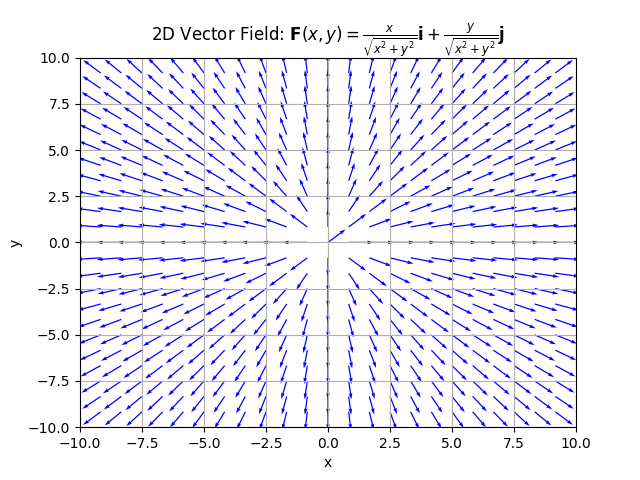
\includegraphics[width=0.8\textwidth]{chapters/chp5_pics/5.1.1-1.png}
\label{fig:5.1.1-1}
\end{figure}
   
   This is a \textbf{source field} with unit vectors. All vectors point outward from the origin with equal magnitude. It's similar to the electric field of a positive point charge or the field lines emerging from a magnetic monopole (if one existed).
   
\item For $\mathbf{F}(x,y) = \frac{x^2-y^2}{\sqrt{(x^2-y^2)^2 + (2xy)^2}}\mathbf{i} + \frac{2xy}{\sqrt{(x^2-y^2)^2 + (2xy)^2}}\mathbf{j}$

This normalized version of our previous field will help us understand its pure directional behavior. At each point, we're taking the same direction but scaling it to have unit length. Let's understand how we got here:

\begin{itemize}
   \item The original field was $\mathbf{F}(x,y) = (x^2-y^2)\mathbf{i} + (2xy)\mathbf{j}$
   \item Its magnitude at any point is $\sqrt{(x^2-y^2)^2 + (2xy)^2}$
   \item Dividing by this magnitude normalizes each vector to length 1
\end{itemize}

Let's evaluate at carefully chosen points. Since we're normalizing, what matters most is the ratio between components rather than their absolute values:

\begin{center}
\begin{tabular}{|c|c||c|c|c|}
\hline
$(x,y)$ & $\sqrt{(x^2-y^2)^2 + (2xy)^2}$ & $P(x,y)$ & $Q(x,y)$ & Direction \\
\hline
$(1,0)$ & 1 & 1 & 0 & Right \\
$(1,1)$ & 2 & 0 & 1 & Up \\
$(0,1)$ & 1 & -1 & 0 & Left \\
$(-1,1)$ & 2 & 0 & -1 & Down \\
$(-1,0)$ & 1 & 1 & 0 & Right \\
$(-1,-1)$ & 2 & 0 & 1 & Up \\
$(0,-1)$ & 1 & -1 & 0 & Left \\
$(1,-1)$ & 2 & 0 & -1 & Down \\
\hline
\end{tabular}
\end{center}

Let's sketch these unit vectors, being careful to show points at different distances from the origin:

\begin{center}
\begin{tikzpicture}[scale=2]
% Draw axes
\draw[->] (-2,0) -- (2,0) node[right] {$x$};
\draw[->] (0,-2) -- (0,2) node[above] {$y$};

% Draw unit vectors (all length 1)
\draw[blue,thick,->] (1,1) -- (1,2);
\draw[blue,thick,->] (1,-1) -- (1,-2);
\draw[blue,thick,->] (1,0) -- (2,0);
\draw[blue,thick,->] (0,1) -- (-1,1);
\draw[blue,thick,->] (2,1) -- (2.6,1.8);
\draw[blue,thick,->] (1.414,1.414) -- (1.414,2.414);  % √2 points
\draw[blue,thick,->] (2,0) -- (3,0);
\draw[blue,thick,->] (0,2) -- (-1,2);
\draw[blue,thick,->] (2,-1) -- (2.6,-1.8);
\draw[blue,thick,->] (0.707,0.707) -- (0.707,1.707);  % 1/√2 points

% Label points
\fill (1,1) circle (1pt) node[above right] {\tiny$(1,1)$};
\fill (1,0) circle (1pt) node[below] {\tiny$(1,0)$};
\fill (2,1) circle (1pt) node[right] {\tiny$(2,1)$};
\fill (1.414,1.414) circle (1pt) node[above right] {\tiny$(\sqrt{2},\sqrt{2})$};
\fill (2,0) circle (1pt) node[below] {\tiny$(2,0)$};
\fill (0.707,0.707) circle (1pt) node[above left] {\tiny$(\frac{1}{\sqrt{2}},\frac{1}{\sqrt{2}})$};

% Label origin
\node at (0,0) {$\bullet$};
\node[below right] at (0,0) {$O$};
\end{tikzpicture}
\end{center}

These additional points help reveal even more patterns in the field:
\begin{itemize}
   \item The same directional pattern appears at all distances from the origin - notice how points like $(1,1)$ and $(\frac{1}{\sqrt{2}},\frac{1}{\sqrt{2}})$ show identical behavior despite being at different distances
   \item Along rays from the origin (like the points $(1,0)$ and $(2,0)$), vectors point in exactly the same direction
   \item The transition between vertical and horizontal flow is smooth and consistent at all distances
   \item Each point's vector direction depends only on the ratio of $y$ to $x$, not on their absolute values
\end{itemize}

The computer-generated vector field looks like this:

\begin{figure}[H]
\centering
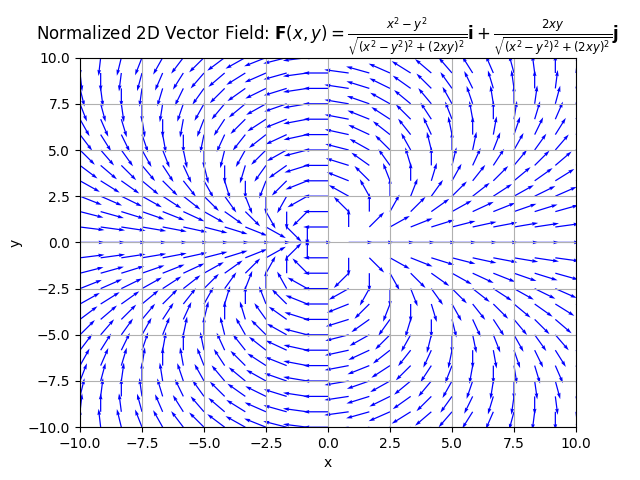
\includegraphics[width=0.8\textwidth]{chapters/chp5_pics/5.1.1-2.png}
\label{fig:5.1.1-2}
\end{figure}

This normalized version of the field reveals its pure directional behavior. Now we can see clearly how the field creates a twisted circulation pattern, with vectors smoothly transitioning between vertical flow along diagonals and horizontal flow near the axes. This type of normalization is often useful in physics when we care more about the direction of a force or flow than its magnitude, such as in studying the directional patterns of complex fluid flows.
\end{enumerate}
\end{solution}
\end{example}
\exampleline

\subsection*{Conservative Vector Fields} \index{Conservative Fields}

\noindent When studying vector fields, one of the most fundamental questions we can ask is whether the field represents a quantity that depends only on position, or one that depends on how we got to that position. This distinction leads us to the crucial concept of conservative vector fields. \\

\noindent A vector field $\mathbf{F}$ is called \textbf{conservative} if there exists a scalar function $f$, called a \textbf{potential function}, such that:
\[
\mathbf{F} = \nabla f
\]

\noindent In two dimensions, this means:
\[
P(x,y) = \frac{\partial f}{\partial x} \quad \text{and} \quad Q(x,y) = \frac{\partial f}{\partial y}
\]

\noindent And in three dimensions:
\[
P(x,y,z) = \frac{\partial f}{\partial x}, \quad Q(x,y,z) = \frac{\partial f}{\partial y}, \quad \text{and} \quad R(x,y,z) = \frac{\partial f}{\partial z}
\]

\noindent The term ``conservative" comes from the fact that these fields conserve energy—there's no loss or gain of energy when moving along a closed path. This leads to several critical properties:

\begin{itemize}
   \item The work done by a conservative field along any path between two points depends only on the endpoints, not on the path taken
   \item The curl of a conservative field is zero (a fact we'll explore in detail later)
   \item Line integrals of conservative fields around closed paths are always zero
\end{itemize}

\noindent When a field is not conservative, we call it \textbf{non-conservative} or \textbf{rotational}. Understanding whether a field is conservative or non-conservative has profound implications in physics and engineering:

\begin{itemize}
   \item \textbf{Conservative Fields:}
       \begin{itemize}
           \item Gravitational fields
           \item Electrostatic fields
           \item Pressure gradients in static fluids
       \end{itemize}
       
   \item \textbf{Non-Conservative Fields:} \index{Non-Conservative Fields}
       \begin{itemize}
           \item Magnetic fields
           \item Friction forces
           \item Velocity fields in rotating fluids
       \end{itemize}
\end{itemize}

\subsection*{Testing for Conservative Fields}

\noindent Not all vector fields are conservative. The key test involves examining the field's partial derivatives. In two dimensions, if $\mathbf{F}(x,y) = P\mathbf{i} + Q\mathbf{j}$ is defined on a simply connected domain, then $\mathbf{F}$ is conservative if and only if:
\[
\frac{\partial P}{\partial y} = \frac{\partial Q}{\partial x}
\]

\noindent This condition arises from the equality of mixed partial derivatives of the potential function:
\[
\frac{\partial^2 f}{\partial y\partial x} = \frac{\partial^2 f}{\partial x\partial y}
\]

\noindent In three dimensions, a vector field $\mathbf{F}(x,y,z) = P\mathbf{i} + Q\mathbf{j} + R\mathbf{k}$ defined on a simply connected domain is conservative if and only if:
\[
\frac{\partial P}{\partial y} = \frac{\partial Q}{\partial x}, \quad
\frac{\partial P}{\partial z} = \frac{\partial R}{\partial x}, \quad
\frac{\partial Q}{\partial z} = \frac{\partial R}{\partial y}
\]

\noindent The significance of conservative fields extends far beyond these mathematical conditions. Consider these practical implications:

\begin{enumerate}
   \item \textbf{Energy Conservation:} In conservative systems, energy is perfectly conserved. A ball rolling in a gravitational field (ignoring friction) will reach the same height regardless of the path it takes.
   
   \item \textbf{Path Independence:} The work done by conservative forces depends only on start and end positions. This means we can choose the most convenient path for our calculations.
   
   \item \textbf{Potential Functions:} Conservative fields allow us to define potential energy functions, greatly simplifying many physical calculations. Instead of computing complicated path integrals, we can just evaluate the potential function at endpoints.
   
   \item \textbf{Equilibrium Analysis:} The existence of a potential function helps identify stable and unstable equilibrium points in physical systems.
\end{enumerate}

\noindent In contrast, non-conservative fields exhibit fundamentally different behavior:
\begin{enumerate}
   \item They can do different amounts of work along different paths
   \item They can add or remove energy from a system
   \item They often represent dissipative forces or fields that depend on velocity
   \item They cannot be derived from a potential function
\end{enumerate}

\noindent This distinction between conservative and non-conservative fields is crucial in physics and engineering. For instance, when designing energy systems, knowing whether forces are conservative helps predict whether energy will be conserved or dissipated. In fluid dynamics, identifying non-conservative velocity fields helps understand where energy losses occur. Even in economics, conservative fields can model ideal market behaviors, while non-conservative fields might better represent real markets with friction and inefficiencies.


\exampleline
\begin{example}
Let's see what kind of fields Example 5.1.1 had (with the second example being changed to non-normalized for ease of differentiation). Please classify them as either Conservative or Non-Conservative:

\begin{enumerate}
   \item The normalized radial field $\mathbf{F}(x,y) = \frac{x}{\sqrt{x^2+y^2}}\mathbf{i} + \frac{y}{\sqrt{x^2+y^2}}\mathbf{j}$
   
   \item The quadratic field $\mathbf{F}(x,y) = (x^2-y^2)\mathbf{i} + (2xy)\mathbf{j}$
\end{enumerate}

Determine whether each field is conservative by testing the condition $\frac{\partial P}{\partial y} = \frac{\partial Q}{\partial x}$.

\begin{solution}
Let's analyze each field systematically:

\begin{enumerate}
   \item For the normalized radial field, let:
   \[
   P(x,y) = \frac{x}{\sqrt{x^2+y^2}} \quad \text{and} \quad Q(x,y) = \frac{y}{\sqrt{x^2+y^2}}
   \]
   
   First, compute $\frac{\partial P}{\partial y}$ using the quotient rule:
   \begin{align*}
   \frac{\partial P}{\partial y} &= \frac{\partial}{\partial y}\left(\frac{x}{\sqrt{x^2+y^2}}\right) \\
   &= x \cdot \frac{\partial}{\partial y}\left(\frac{1}{\sqrt{x^2+y^2}}\right) \\
   &= x \cdot \left(-\frac{1}{2}(x^2+y^2)^{-3/2} \cdot 2y\right) \\
   &= -\frac{xy}{(x^2+y^2)^{3/2}}
   \end{align*}
   
   Next, compute $\frac{\partial Q}{\partial x}$:
   \begin{align*}
   \frac{\partial Q}{\partial x} &= \frac{\partial}{\partial x}\left(\frac{y}{\sqrt{x^2+y^2}}\right) \\
   &= y \cdot \frac{\partial}{\partial x}\left(\frac{1}{\sqrt{x^2+y^2}}\right) \\
   &= y \cdot \left(-\frac{1}{2}(x^2+y^2)^{-3/2} \cdot 2x\right) \\
   &= -\frac{xy}{(x^2+y^2)^{3/2}}
   \end{align*}
   
   Since $\frac{\partial P}{\partial y} = \frac{\partial Q}{\partial x}$, this field is conservative. Indeed, we can find its potential function: $f(x,y) = \sqrt{x^2+y^2}$. This explains why this normalized field points radially outward—it represents the direction of steepest increase of the distance function from the origin.
   
   \item For the quadratic field, let:
   \[
   P(x,y) = x^2-y^2 \quad \text{and} \quad Q(x,y) = 2xy
   \]
   
   Computing the partial derivatives:
   \begin{align*}
   \frac{\partial P}{\partial y} &= \frac{\partial}{\partial y}(x^2-y^2) = -2y \\
   \frac{\partial Q}{\partial x} &= \frac{\partial}{\partial x}(2xy) = 2y
   \end{align*}
   
   Since $\frac{\partial P}{\partial y} = -2y \neq 2y = \frac{\partial Q}{\partial x}$, this field is non-conservative. This aligns with our earlier observation of its rotational behavior—the field exhibits a circulation pattern that cannot be derived from any potential function. If we were to compute the work done by this field along different paths between the same points, we would get different results.
\end{enumerate}
\end{solution}
\end{example}
\exampleline











\newpage

\lecture{Line Integrals} \index{Line Integrals}

\noindent After our exploration of vector fields, we now turn to one of the most fundamental operations we can perform on them: integration along curves. Just as we previously extended single-variable integration to multiple dimensions through multiple integrals, we'll now develop the tools to integrate both scalar functions and vector fields along paths in space. This concept will prove crucial in physics, engineering, and advanced mathematics.

\subsection*{Line Integrals of Scalar Functions}

\noindent Before diving into vector fields, let's start with a simpler scenario: integrating a scalar function along a curve. Imagine walking along a curved path on a hilly terrain. At each point, there's an elevation—a scalar value associated with your position. If we wanted to calculate the ``total elevation" experienced along our path, we'd need a line integral. \\

\noindent Recall from Chapter 2 Lecture 4 that we developed the concept of arc length for a parametric curve. Given a curve $C$ parameterized by $\mathbf{r}(t) = x(t)\mathbf{i} + y(t)\mathbf{j}$ for $a \leq t \leq b$, we found its length using:
\[
L = \int_a^b \sqrt{\left(\frac{dx}{dt}\right)^2 + \left(\frac{dy}{dt}\right)^2}\,dt = \int_a^b \left\|\frac{d\mathbf{r}}{dt}\right\|\,dt
\]

\noindent Now imagine that at each point along this curve, we're not just measuring distance but also evaluating some scalar function $f(x,y)$. We can think of this as ``weighting" each infinitesimal piece of arc length by the value of $f$ at that point. This leads naturally to the line integral:
\[
\int_C f(x,y)\,ds = \int_a^b f(x(t),y(t))\sqrt{\left(\frac{dx}{dt}\right)^2 + \left(\frac{dy}{dt}\right)^2}\,dt
\]
\noindent We note that this will yield us an area, because we are multiplying the arc length by a height function. Let's break down the components of this integral:
\begin{itemize}
    \item $f(x(t),y(t))$ evaluates our scalar function at each point along $C$
    \item $\sqrt{\left(\frac{dx}{dt}\right)^2 + \left(\frac{dy}{dt}\right)^2}\,dt$ gives us the infinitesimal arc length $ds$
    \item Their product $f(x(t),y(t))\,ds$ represents the contribution of each tiny piece of the curve
\end{itemize}

\noindent This geometric interpretation helps us understand several key properties:

\begin{enumerate}
    \item \textbf{Reparametrization Invariance:} The value of the line integral doesn't depend on how we parameterize $C$. Different parameters will adjust both $f(x(t),y(t))$ and $\frac{d\mathbf{r}}{dt}$, but their product remains constant.
    
    \item \textbf{Direction Independence:} For scalar line integrals, the direction we traverse $C$ doesn't matter. This is because $ds$ is always positive, measuring pure distance rather than directed movement.

\begin{figure}[H]
\centering
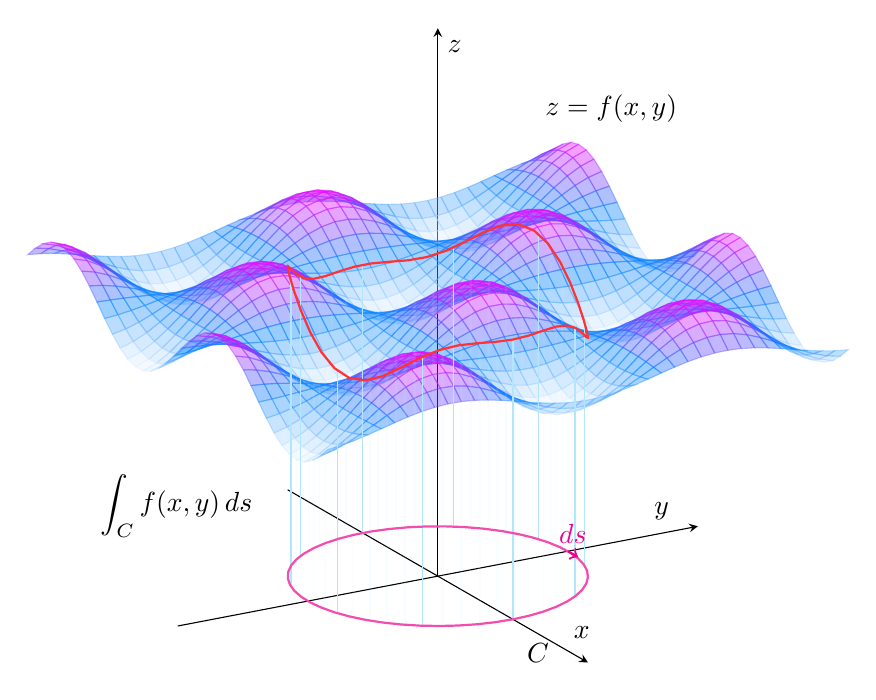
\begin{tikzpicture}
\begin{axis}[
    view={60}{20},  % Adjusted view angle for better visibility underneath
    axis lines=middle,
    xlabel={$x$},
    ylabel={$y$},
    zlabel={$z$},
    grid=none,
    ticks=none,
    width=12cm,
    height=12cm,
    xmin=-3, xmax=3,
    ymin=-3, ymax=3,
    zmin=0, zmax=4,  % Lifted up the z-range
    samples=40,
    domain=-3:3,
    y domain=-3:3,
    colormap/cool,
    clip=false
]

% Draw the undulating surface
\addplot3[
    surf,
    faceted color=blue!10,  % Made surface color lighter
    opacity=0.4,  % More transparent
    shader=flat,
] {2 + 0.3*sin(deg(2*x))*cos(deg(2*y))};  % Centered and lifted surface

% Fill the area under the curve with semi-transparent sheets
\pgfplotsinvokeforeach{0,0.02,...,1}{
    % Create fill between curve and xy-plane
    \addplot3[
        fill=cyan!20,  % Light cyan fill
        opacity=0.1,  % Very transparent for layered effect
        draw=none
    ] coordinates {
        ({1.5*cos(360*#1)}, {1.5*sin(360*#1)}, 0)
        ({1.5*cos(360*#1)}, {1.5*sin(360*#1)}, {2 + 0.3*sin(deg(3*cos(360*#1)))*cos(deg(3*sin(360*#1)))})
        ({1.5*cos(360*#1 + 1)}, {1.5*sin(360*#1 + 1)}, {2 + 0.3*sin(deg(3*cos(360*#1 + 1)))*cos(deg(3*sin(360*#1 + 1)))})
        ({1.5*cos(360*#1 + 1)}, {1.5*sin(360*#1 + 1)}, 0)
    };
}

% Draw vertical lines for the "curtain" effect
\pgfplotsinvokeforeach{0,0.1,...,1}{
    \addplot3[cyan!30, thin] coordinates {
        ({1.5*cos(360*#1)}, {1.5*sin(360*#1)}, 0)
        ({1.5*cos(360*#1)}, {1.5*sin(360*#1)}, {2 + 0.3*sin(deg(3*cos(360*#1)))*cos(deg(3*sin(360*#1)))})
    };
}

% Draw the curve on the surface
\addplot3[
    red!80,  % Slightly dimmer red
    thick,
    samples=50,
    domain=0:360,
] ({1.5*cos(x)}, {1.5*sin(x)}, {2 + 0.3*sin(deg(3*cos(x)))*cos(deg(3*sin(x)))});

% Draw the projected curve on xy-plane
\addplot3[
    magenta!70,  % Dimmer magenta
    thick,
    dashed,
    samples=50,
    domain=0:360,
] ({1.5*cos(x)}, {1.5*sin(x)}, 0);

% Add labels
\node[anchor=north] at (axis cs:2,0,0) {$C$};
\node[anchor=south] at (axis cs:0,2,3) {$z=f(x,y)$};
\node[anchor=west] at (axis cs:0,-4,1) {$\displaystyle\int_C f(x,y)\,ds$};

% Add a small ds element indicator
\draw[magenta,->,thick] (axis cs:0,1.5,0) -- (axis cs:0.2,1.5,0) node[midway,above] {$ds$};

\end{axis}
\end{tikzpicture}
\caption{\textit{Geometric interpretation of a scalar line integral $\int_C f(x,y)\,ds$. The curve $C$ (shown in red) lies on the surface $z=f(x,y)$, while its projection onto the $xy$-plane is shown as a dashed magenta curve. The shaded ``curtain" between these curves represents the accumulation of the function values along the path, with each vertical height $f(x,y)$ being weighted by the infinitesimal arc length $ds$.}}
\label{fig:scalar_line_integral}
\end{figure}
    
    \item \textbf{Physical Meaning:} The integral accumulates the product of the scalar field and distance traveled, giving us meaningful physical quantities:
    \begin{itemize}
        \item Mass = $\int_C \rho(x,y)\,ds$ where $\rho$ is linear density
        \item Cost = $\int_C c(x,y)\,ds$ where $c$ is cost per unit length
        \item Average value of $f$ along $C$ = $\frac{1}{L}\int_C f(x,y)\,ds$ where $L$ is the arc length
    \end{itemize}
\end{enumerate}

\noindent The computation process follows these steps:
\begin{enumerate}
    \item Express the curve $C$ parametrically: $\mathbf{r}(t) = x(t)\mathbf{i} + y(t)\mathbf{j}$
    \item Calculate $\frac{dx}{dt}$ and $\frac{dy}{dt}$
    \item Compose $f$ with the parametrization: $f(x(t),y(t))$
    \item Form the integrand: $f(x(t),y(t))\sqrt{\left(\frac{dx}{dt}\right)^2 + \left(\frac{dy}{dt}\right)^2}$
    \item Integrate with respect to $t$ from $a$ to $b$
\end{enumerate}


\noindent You may encounter an alternative notation for line integrals, particularly in complex analysis and physics: the contour integral. Written as $\oint_C f(x,y)\,ds$, this notation emphasizes that we're integrating along a specific path or contour in the plane. The circle in the integral symbol traditionally suggests a closed path—one that returns to its starting point. While we'll primarily use $\int_C$ notation in our development of vector calculus, recognizing the contour notation is crucial as it appears frequently in applications, especially when dealing with conservative fields and path independence. \\

\exampleline
\begin{example}
Evaluate the line integral $\int_C f(x,y)\,ds$ where $f(x,y) = y-2x$ along:
\begin{enumerate}
    \item The curve $C_1$ given by $\mathbf{r}(t) = (2t)\mathbf{i} + (3t)\mathbf{j}$, $0 \leq t \leq 1$
    \item The curve $C_2$ given by $\mathbf{r}(t) = (\cos t)\mathbf{i} + (2\sin t)\mathbf{j}$, $0 \leq t \leq 2\pi$
\end{enumerate}
\begin{solution}
Let's evaluate each integral systematically:
\begin{enumerate}
    \item For curve $C_1$:
    
    First, we need:
    \begin{itemize}
        \item $\frac{dx}{dt} = 2$, $\frac{dy}{dt} = 3$
        \item $f(x(t),y(t)) = 3t-4t = -t$ 
        \item $ds = \sqrt{(\frac{dx}{dt})^2 + (\frac{dy}{dt})^2}\,dt = \sqrt{4+9}\,dt = \sqrt{13}\,dt$
    \end{itemize}
    
    Therefore:
    \begin{align*}
        \int_C f(x,y)\,ds &= \int_0^1 (-t)(\sqrt{13})\,dt \\
        &= -\sqrt{13}\int_0^1 t\,dt \\
        &= -\sqrt{13}[\frac{t^2}{2}]_0^1 \\
        &= -\frac{\sqrt{13}}{2}
    \end{align*}
    
    \item For curve $C_2$:
    
    We need:
    \begin{itemize}
        \item $\frac{dx}{dt} = -\sin t$, $\frac{dy}{dt} = 2\cos t$
        \item $f(x(t),y(t)) = 2\sin t - 2\cos t$
        \item $ds = \sqrt{(\frac{dx}{dt})^2 + (\frac{dy}{dt})^2}\,dt = \sqrt{\sin^2 t + 4\cos^2 t}\,dt$
    \end{itemize}
    
    Therefore:
    \begin{align*}
        \oint_C f(x,y)\,ds &= \int_0^{2\pi} (2\sin t - 2\cos t)\sqrt{\sin^2 t + 4\cos^2 t}\,dt \\
        &= 0
    \end{align*}
	We see in this example where the height function goes negative for part of the region, and thus the total area is 0 from equal positive and negative contributions.
\end{enumerate}
\end{solution}
\end{example}
\exampleline

\subsection*{Contours}

\noindent To evaluate line integrals effectively, we need a systematic understanding of the curves—or contours—along which we integrate; we will not always be given the parameterization of the curve like in the last two examples. A contour in the plane is simply a continuous curve that can be parameterized, but the nature of these curves (whether they're open or closed, smooth or piecewise) significantly impacts our computational approach. \\

\noindent \textbf{Definition:} A \textit{contour} $C$ is a curve in the plane that can be described by a continuous vector-valued function $\mathbf{r}(t) = x(t)\mathbf{i} + y(t)\mathbf{j}$ over some interval $[a,b]$. We classify contours into several types:

\begin{itemize}
    \item \textbf{Open Contours:} Curves where the endpoints are distinct: $\mathbf{r}(a) \neq \mathbf{r}(b)$
    \item \textbf{Closed Contours:} Curves that return to their starting point: $\mathbf{r}(a) = \mathbf{r}(b)$
    \item \textbf{Simple Contours:} Curves that don't intersect themselves (except possibly at endpoints)
    \item \textbf{Piecewise Contours:} Curves composed of multiple smooth segments
\end{itemize}

\begin{figure}[H]
\centering
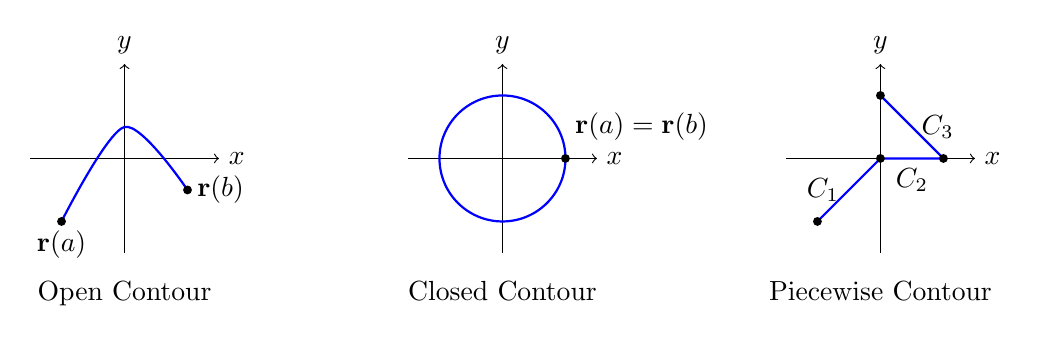
\begin{tikzpicture}[scale=0.8]
    % Open Contour
    \begin{scope}[xshift=-6cm]
        \draw[->] (-1.5,0) -- (1.5,0) node[right] {$x$};
        \draw[->] (0,-1.5) -- (0,1.5) node[above] {$y$};
        \draw[blue, thick] plot[smooth] coordinates {(-1,-1) (0,0.5) (1,-0.5)};
        \fill (-1,-1) circle (2pt) node[below] {$\mathbf{r}(a)$};
        \fill (1,-0.5) circle (2pt) node[right] {$\mathbf{r}(b)$};
        \node[below] at (0,-1.8) {Open Contour};
    \end{scope}
    
    % Closed Contour
    \begin{scope}[xshift=0cm]
        \draw[->] (-1.5,0) -- (1.5,0) node[right] {$x$};
        \draw[->] (0,-1.5) -- (0,1.5) node[above] {$y$};
        \draw[blue, thick] (1,0) arc (0:360:1);
        \fill (1,0) circle (2pt) node[right] {};
        \fill (1,0.5) circle (0pt) node[right] {$\mathbf{r}(a)=\mathbf{r}(b)$};
        \node[below] at (0,-1.8) {Closed Contour};
    \end{scope}
    
    % Piecewise Contour
    \begin{scope}[xshift=6cm]
        \draw[->] (-1.5,0) -- (1.5,0) node[right] {$x$};
        \draw[->] (0,-1.5) -- (0,1.5) node[above] {$y$};
        \draw[blue, thick] (-1,-1) -- (0,0) -- (1,0) -- (0,1);
        \fill (-1,-1) circle (2pt);
        \fill (0,0) circle (2pt);
        \fill (1,0) circle (2pt);
        \fill (0,1) circle (2pt);
        \node[left] at (-0.5,-0.5) {$C_1$};
        \node[below] at (0.5,0) {$C_2$};
        \node[right] at (0.5,0.5) {$C_3$};
        \node[below] at (0,-1.8) {Piecewise Contour};
    \end{scope}
\end{tikzpicture}
\caption{\textit{Different types of contours. The piecewise contour shows junction points where segments meet.}}
\label{fig:contour_types}
\end{figure}

\noindent To work with these contours, we need appropriate parameterizations. Here are the fundamental parameterizations that form our computational toolkit:

\begin{table}[htb]
\caption{Common Parameterized Curves in Line Integrals and Their Arc Length Elements}
\begin{center}
\small
\begin{tabular}{|p{2.5cm}|p{4.5cm}|p{3cm}|p{4cm}|}
\hline
\rule{0pt}{4ex}\textbf{Curve Type} & \textbf{Parameterization} & \textbf{Parameter Range} & \textbf{Arc Length Element} \rule[-2ex]{0pt}{0pt}\\
\hline
\rule{0pt}{5ex}Line Segment &
$\mathbf{r}(t) = (1-t)(x_1,y_1) + t(x_2,y_2)$ \newline
or \newline
$(x_1 + t(x_2-x_1),\ y_1 + t(y_2-y_1))$ &
$0 \leq t \leq 1$ &
$ds = \sqrt{(\Delta x)^2 + (\Delta y)^2}\,dt$ \rule[-2.5ex]{0pt}{0pt}\\
\hline
\rule{0pt}{4ex}Circle &
$\mathbf{r}(t) = (a + r\cos t,\ b + r\sin t)$ &
$0 \leq t \leq 2\pi$ &
$ds = r\,dt$ \rule[-2ex]{0pt}{0pt}\\
\hline
\rule{0pt}{4ex}Circular Arc &
$\mathbf{r}(t) = (a + r\cos t,\ b + r\sin t)$ &
$\alpha \leq t \leq \beta$ &
$ds = r\,dt$ \rule[-2ex]{0pt}{0pt}\\
\hline
\rule{0pt}{4ex}Ellipse &
$\mathbf{r}(t) = (a\cos t,\ b\sin t)$ &
$0 \leq t \leq 2\pi$ &
$ds = \sqrt{a^2\sin^2 t + b^2\cos^2 t}\,dt$ \rule[-2ex]{0pt}{0pt}\\
\hline
\rule{0pt}{4ex}Parabola &
$\mathbf{r}(t) = (t,\ at^2)$ &
$t_1 \leq t \leq t_2$ &
$ds = \sqrt{1 + 4a^2 t^2}\,dt$ \rule[-2ex]{0pt}{0pt}\\
\hline
\rule{0pt}{4ex}Any Function &
$\mathbf{r}(t) = (t,\ f(t))$ &
$t_1 \leq t \leq t_2$ &
$ds = \sqrt{1 + \left(f'(t)\right)^2}\,dt$ \rule[-2ex]{0pt}{0pt}\\
\hline
\end{tabular}
\end{center}
\label{tab:curve-parameterizations}
\end{table}

\noindent For piecewise contours, we use the principle of additivity: when a contour $C$ is composed of several pieces $C_1, C_2, \ldots, C_n$, we can break down the integral:
\[
\int_C f(x,y)\,ds = \sum_{i=1}^n \int_{C_i} f(x,y)\,ds
\]

\noindent This fundamental property transforms complex integration problems into a series of simpler calculations over basic curves. When working with piecewise contours:

\begin{enumerate}
    \item Identify the junction points where different segments meet
    \item Choose appropriate parameterizations for each segment
    \item Ensure consistent orientation throughout the contour
    \item Apply the additivity principle to sum the contributions
\end{enumerate}

\begin{figure}[H]
\centering
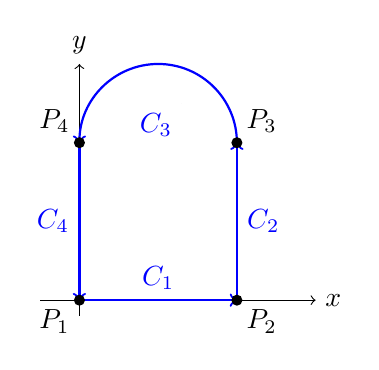
\begin{tikzpicture}
    % Example of breaking down a complex contour
    \draw[->] (-0.5,0) -- (3,0) node[right] {$x$};
    \draw[->] (0,-0.2) -- (0,3) node[above] {$y$};
    
    % Draw a complex piecewise contour
    \draw[blue, thick, ->] (0,0) -- node[above] {$C_1$} (2,0);
    \draw[blue, thick, ->] (2,0) -- node[right] {$C_2$} (2,2);
    \draw[blue, thick, ->] (2,2) arc (0:180:1) node[above] {};
    \draw[blue, thick, ->] (0,2) -- node[left] {$C_4$} (0,0);
    
    % Add points
    \fill (0,0) circle (2pt) node[below left] {$P_1$};
    \fill (2,0) circle (2pt) node[below right] {$P_2$};
    \fill (2,2) circle (2pt) node[above right] {$P_3$};
    \fill (0,2) circle (2pt) node[above left] {$P_4$};

\fill (1.3,2.5) circle (0pt) node[below left, text=blue] {$C_3$};

\end{tikzpicture}
\caption{\textit{Breaking down a complex contour into basic elements: line segments ($C_1$, $C_2$, $C_4$) and a circular arc ($C_3$). The arrows indicate the orientation of integration.}}
\label{fig:complex_contour}
\end{figure}

\noindent The choice of parameterization affects our calculations but not the final result. When selecting parameterizations:

\begin{itemize}
    \item Choose parameterizations that simplify the integrand when possible
    \item Ensure smooth transitions at junction points
    \item Consider symmetry to simplify calculations
    \item Remember that different parameterizations of the same curve yield the same integral value
\end{itemize}

\noindent This systematic approach to understanding and working with contours provides the foundation for evaluating line integrals in practice. Whether we're computing work done by a force field or finding the mass of a curved wire, these tools allow us to break complex problems into manageable pieces.



\exampleline
\begin{example}
Consider the scalar function $f(x,y) = x^2 + y$.

\begin{enumerate}
\item Compute $\int_C f(x,y)\,ds$ where $C$ is the path from $(0,0)$ to $(1,1)$ consisting of:
\begin{itemize}
\item A quarter circle of radius 1 from $(0,0)$ to $(1,0)$
\item A vertical line segment from $(1,0)$ to $(1,1)$
\end{itemize}

\item Compute $\int_C f(x,y)\,ds$ where $C$ is the curve $y = x^2$ from $(0,0)$ to $(1,1)$.
\end{enumerate}

\begin{solution}
\begin{enumerate}
\item Let's break this into two parts using $\int_C f(x,y)\,ds = \int_{C_1} f(x,y)\,ds + \int_{C_2} f(x,y)\,ds$

\begin{figure}[H]
\centering
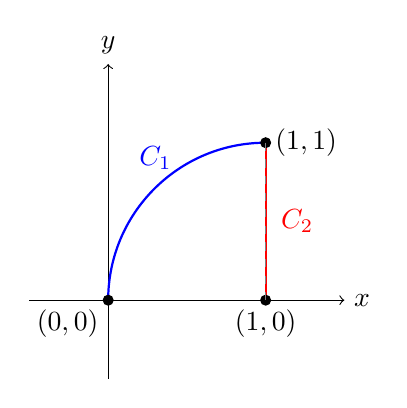
\begin{tikzpicture}[scale=2]
    % Grid and axes
    \draw[->] (-0.5,0) -- (1.5,0) node[right] {$x$};
    \draw[->] (0,-0.5) -- (0,1.5) node[above] {$y$};
    
    % Quarter circle with center at (1,1)
    \draw[blue, thick] (0,0) arc (180:90:1);
    
    % Vertical line
    \draw[red, thick] (1,0) -- (1,1);
    
    % Points
    \fill (0,0) circle (1pt) node[below left] {$(0,0)$};
    \fill (1,0) circle (1pt) node[below] {$(1,0)$};
    \fill (1,1) circle (1pt) node[right] {$(1,1)$};
    
    % Center point of circle
    \fill[black] (1,1) circle (0.5pt) node[above right] {};
    \draw[dashed, gray] (1,1) -- (1,0);
    
    % Labels
    \node[blue] at (0.3,0.9) {$C_1$};
    \node[red] at (1.2,0.5) {$C_2$};
\end{tikzpicture}
\caption{\textit{The piecewise path consisting of a quarter circle ($C_1$) centered at $(1,0)$ followed by a vertical line segment ($C_2$).}}
\label{fig:piecewise_path}
\end{figure}

For $C_1$ (quarter circle):
\begin{itemize}
\item Parameterization: $\mathbf{r}(t) = (1 + \cos t)\mathbf{i} +\sin t\mathbf{j}$, $\frac{\pi}{2} \leq t \leq \pi$
\item $\frac{dx}{dt} = -\sin t$, $\frac{dy}{dt} = \cos t$
\item $ds = \sqrt{(-\sin t)^2 + (\cos t)^2}\,dt = dt$
\item $f(x(t),y(t)) = (1 + \cos t)^2 + (\sin t) = 1 + 2\cos t + \cos^2 t + \sin t$
\end{itemize}

The integral over $C_1$ becomes:
\[
\int_{C_1} f(x,y)\,ds = \int_{\pi/2}^{\pi} (1 + 2\cos t + \cos^2 t + \sin t)\,dt = \frac{3\pi}{4} - 1 \approx 1.3562
\]

For $C_2$ (vertical line):
\begin{itemize}
\item Parameterization: $\mathbf{r}(t) = \mathbf{i} + t\mathbf{j}$, $0 \leq t \leq 1$
\item $f(x(t),y(t)) = 1 + t$
\item $ds = dt$
\end{itemize}

Therefore:
\begin{align*}
\int_{C_2} f(x,y)\,ds &= \int_0^1 (1 + t)\,dt \\
&= [t + \frac{t^2}{2}]_0^1 = \frac{3}{2}
\end{align*}

The total integral is the sum $\frac{3\pi}{4} - 1 + \frac{3}{2} \approx 2.8562.$

\item For the parabola $y = x^2$:

\begin{figure}[H]
\centering
\begin{tikzpicture}[scale=2]
    % Grid and axes
    \draw[->] (-0.5,0) -- (1.5,0) node[right] {$x$};
    \draw[->] (0,-0.5) -- (0,1.5) node[above] {$y$};
    
    % Parabola
    \draw[blue, thick] plot[domain=0:1] (\x, \x*\x);
    
    % Points
    \fill (0,0) circle (1pt) node[below left] {$(0,0)$};
    \fill (1,1) circle (1pt) node[right] {$(1,1)$};
    
    % Label
    \node[blue] at (0.7,0.3) {$C$};
\end{tikzpicture}
\caption{\textit{The parabolic path $y=x^2$.}}
\label{fig:parabola_path}
\end{figure}

\begin{itemize}
\item Parameterization: $\mathbf{r}(t) = t\mathbf{i} + t^2\mathbf{j}$, $0 \leq t \leq 1$
\item $f(x(t),y(t)) = t^2 + t^2 = 2t^2$
\item $\frac{dx}{dt} = 1$, $\frac{dy}{dt} = 2t$
\item $ds = \sqrt{1 + 4t^2}\,dt$
\end{itemize}

The integral does not have a simple closed form:
\[
\int_C f(x,y)\,ds = \int_0^1 2t^2\sqrt{1 + 4t^2}\,dt
\]
We get
\[
\frac{1}{32}\left(18\sqrt{5} - \sinh^{-1}(2)\right) \approx 1.2127
\]
\end{enumerate}
\end{solution}
\end{example}
\exampleline

\subsection*{Line Integrals of Vector Fields}

\noindent We now come to one of the most important distinctions in this chapter. There are \textbf{two fundamentally different types of line integrals}:
\begin{itemize}
\item \textbf{Scalar line integrals} \( \int_C f \, ds \): accumulate a quantity along a path. Think ``total mass of a wire with density \( f \).'' The result is always non-negative (for \( f \geq 0 \)) and does \textit{not} depend on which direction you traverse the curve.
\item \textbf{Vector line integrals} \( \int_C \mathbf{F} \cdot d\mathbf{r} \): measure how much a vector field pushes \textit{along} a path. Think ``work done by a force.'' The result \textit{is} direction-dependent---reversing the path flips the sign.
\end{itemize}
\noindent We spent the previous section on the scalar version. Now we tackle vector line integrals, which are where the real action is.\\ \\
\noindent While scalar line integrals measure accumulation of a scalar quantity along a path, vector field line integrals measure how much a vector field ``works with'' or ``works against'' our motion along a path. This notion arises naturally in physics when computing work done by a force field. \\

\noindent Consider a particle moving through a force field $\mathbf{F}(x,y) = P(x,y)\mathbf{i} + Q(x,y)\mathbf{j}$. At each point, the force vector has both magnitude and direction. The work done by this force depends on:
\begin{itemize}
    \item The strength of the force at each point
    \item How much the force points in our direction of travel
    \item The distance traveled
\end{itemize}

\begin{figure}[H]
    \centering
    \begin{tikzpicture}
        \begin{axis}[
            xmin = -4, xmax = 4,
            ymin = -4, ymax = 4,
            zmin = 0, zmax = 1,
            axis equal image,
            xtick distance = 1,
            ytick distance = 1,
            view = {0}{90},
            scale = 1.25,
            title = {\bf Vector Field: $\vec{F}(x, y) = \left[\frac{-y}{\sqrt{x^2+y^2}}, \frac{x}{\sqrt{x^2+y^2}}\right]$},
            height=7cm,
            xlabel = {$x$},
            ylabel = {$y$},
            colormap/viridis,
            colorbar,
            colorbar style = {
                ylabel = {Distance from Origin}
            }
        ]
            \addplot3[
                point meta = {sqrt(x^2+y^2)},
                quiver = {
                    u = {-y/sqrt(x^2+y^2)},
                    v = {x/sqrt(x^2+y^2)},
                    scale arrows = 0.25,
                },
                quiver/colored = {mapped color},
                -stealth,
                domain = -4:4,
                samples = 21,
                domain y = -4:4,
                samples y = 21,
            ] {0};

            % Line integral path
            \addplot[
                red, very thick,
                postaction = {
                    decorate,
                    decoration = {
                        markings,
                        mark = at position 0.0 with {\arrow[scale=1.5]{>}},
                        mark = at position 0.2 with {\arrow[scale=1.5]{>}},
                        mark = at position 0.4 with {\arrow[scale=1.5]{>}},
                        mark = at position 0.6 with {\arrow[scale=1.5]{>}},
                        mark = at position 0.8 with {\arrow[scale=1.5]{>}}
                    }
                },
                domain = 0:360,
                samples = 100
            ] ({2*cos(x)}, {2*sin(x)});

            \node[above right, red] at (1.5,1.5) {$C$};
        \end{axis}
        \end{tikzpicture}
\caption{\textit{At each point along the path, the contribution to the line integral depends on how much the vector field aligns with the direction of travel.}}
\label{fig:vector_field_integral}
\end{figure}

\noindent This physical intuition leads us to define the line integral of a vector field:
\[
\int_C \mathbf{F} \cdot d\mathbf{r} = \int_C P(x,y)\,dx + Q(x,y)\,dy
\]

\noindent When parameterized by $t$, this becomes:
\[
\int_C \mathbf{F} \cdot d\mathbf{r} = \int_{a}^{b} \mathbf{F}(\mathbf{r}(t))\cdot\mathbf{r}'(t)dt = \int_a^b \left[P(x(t),y(t))\frac{dx}{dt} + Q(x(t),y(t))\frac{dy}{dt}\right]\,dt.
\]
\noindent Or more generally:
\[
\int_C \mathbf{F} \cdot d\mathbf{r} = \int_a^b \left[\sum_{i=1}^n F_i(x_1(t),\ldots,x_n(t))\frac{dx_i}{dt}\right]\,dt
\]

\noindent The dot product $\mathbf{F} \cdot d\mathbf{r}$ captures precisely what we want:
\begin{itemize}
    \item The magnitude of $\mathbf{F}$ affects the contribution
    \item The cosine of the angle between $\mathbf{F}$ and $d\mathbf{r}$ determines how much $\mathbf{F}$ ``helps" or ``hinders" motion
    \item Integration sums these contributions along the entire path
\end{itemize}

\noindent This differs fundamentally from scalar line integrals in several ways:

\begin{enumerate}
    \item \textbf{Direction Matters:} Unlike scalar line integrals where $ds$ is always positive, $d\mathbf{r}$ has direction. Reversing path direction changes the sign of the integral:
    \[
    \int_{-C} \mathbf{F} \cdot d\mathbf{r} = -\int_C \mathbf{F} \cdot d\mathbf{r}
    \]
    \item \textbf{Path Dependence:} The integral may depend on the path taken, not just endpoints. This leads to the rich theory of conservative versus non-conservative fields.
    \item \textbf{Physical Interpretation:} Vector field line integrals naturally represent:
    \begin{itemize}
        \item Work done by force fields
        \item Circulation in fluid flows
        \item Circulation of magnetic fields (Ampere's law)
    \end{itemize}
\end{enumerate}

\noindent The computation process reflects these key differences:
\begin{enumerate}
    \item Parameterize the curve $\mathbf{r}(t)$. Be sure to carefully label the values for which $t$ runs since direction matters.
    \item Calculate $\frac{dx}{dt}$ and $\frac{dy}{dt}$ or for $n$-many dimensions, $\frac{dx_i}{dt}$.
    \item Evaluate $P(x(t),y(t))$ and $Q(x(t),y(t))$ or for $n$-many dimensions, $F_i(x_1(t),\ldots,x_n(t))$. Note: for higher dimensions we denote the unit vector $\mathbf{e}_i$ or $\hat{e}_i$ instead of $\mathbf{i}, \mathbf{j},...$ etc.
    \item Form the integrand $P\frac{dx}{dt} + Q\frac{dy}{dt}$, or for $n$-many dimensions, $\sum_i F_i(x_1(t),\ldots,x_n(t))\frac{dx_i}{dt}$
    \item Integrate with respect to $t$, paying careful attention to orientation
\end{enumerate}


\exampleline
\begin{example}
Consider the vector field $\mathbf{F}(x,y) = \frac{-y}{\sqrt{x^2+y^2}}\mathbf{i} + \frac{x}{\sqrt{x^2+y^2}}\mathbf{j}$. Evaluate $\int_C \mathbf{F}\cdot d\mathbf{r}$ where $C$ is the circle of radius 2 centered at the origin:

\begin{enumerate}
\item Traversed counterclockwise
\item Traversed clockwise
\end{enumerate}

\begin{solution} Let's have a visualization to aid us:

    \begin{figure}[H]
        \centering
        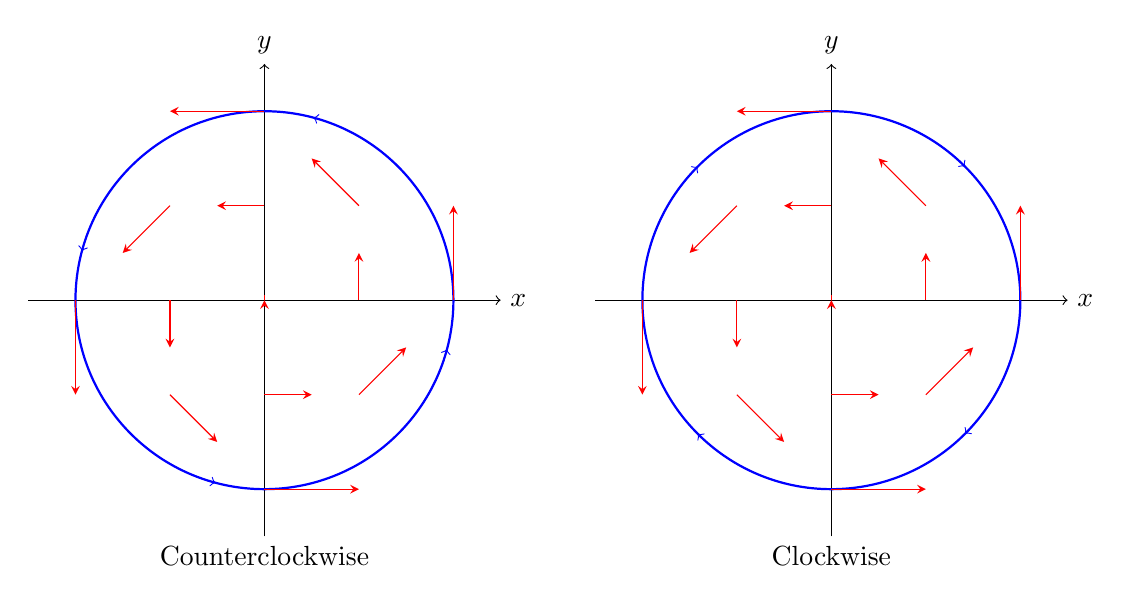
\begin{tikzpicture}[scale=1.2]
            % First subplot: Counterclockwise
            \begin{scope}[xshift=-3cm]
                \draw[->] (-2.5,0) -- (2.5,0) node[right] {$x$};
                \draw[->] (0,-2.5) -- (0,2.5) node[above] {$y$};
                
                % Circle with arrows
                \draw[blue, thick, ->] (0,0) circle (2);
                \foreach \t in {45,135,225,315} {
                    \draw[blue, ->] ({2*cos(\t)},{2*sin(\t)}) arc (\t:\t+30:2);
                }
                
                % Vector field samples
                \foreach \x in {-2,-1,0,1,2} {
                    \foreach \y in {-2,-1,0,1,2} {
                        \ifnum\numexpr\x*\x+\y*\y<5
                            \draw[-stealth, red, thin] (\x,\y) -- +({-\y/2},{+\x/2});
                        \fi
                    }
                }
                
                \node[below] at (0,-2.5) {Counterclockwise};
            \end{scope}
            
            % Second subplot: Clockwise
            \begin{scope}[xshift=3cm]
                \draw[->] (-2.5,0) -- (2.5,0) node[right] {$x$};
                \draw[->] (0,-2.5) -- (0,2.5) node[above] {$y$};
                
                % Circle with arrows
                \draw[blue, thick, <-] (0,0) circle (2);
                \foreach \t in {45,135,225,315} {
                    \draw[blue, <-] ({2*cos(\t)},{2*sin(\t)}) arc (\t:\t+30:2);
                }
                
                % Vector field samples
                \foreach \x in {-2,-1,0,1,2} {
                    \foreach \y in {-2,-1,0,1,2} {
                        \ifnum\numexpr\x*\x+\y*\y<5
                            \draw[-stealth, red, thin] (\x,\y) -- +({-\y/2},{+\x/2});
                        \fi
                    }
                }
                
                \node[below] at (0,-2.5) {Clockwise};
            \end{scope}
        \end{tikzpicture}
        \caption{\textit{The circle $C$ traversed in both directions. The vector field $\mathbf{F}$ (shown in red) is tangent to circles centered at the origin.}}
        \label{fig:circle_directions}
        \end{figure}

\noindent For both cases, we'll parameterize the circle but change our parameter range to reflect direction.

\begin{enumerate}
\item For counterclockwise traversal:
\begin{itemize}
    \item Parameterization: $\mathbf{r}(t) = (2\cos t)\mathbf{i} + (2\sin t)\mathbf{j}$, $0 \leq t \leq 2\pi$
    \item $\frac{dx}{dt} = -2\sin t$, $\frac{dy}{dt} = 2\cos t$
    \item $P(x(t),y(t)) = \frac{-2\sin t}{\sqrt{4\cos^2 t + 4\sin^2 t}} = -\sin t$
    \item $Q(x(t),y(t)) = \frac{2\cos t}{\sqrt{4\cos^2 t + 4\sin^2 t}} = \cos t$
\end{itemize}

Therefore:
\begin{align*}
\int_C \mathbf{F}\cdot d\mathbf{r} &= \int_0^{2\pi} [(-\sin t)(-2\sin t) + (\cos t)(2\cos t)]\,dt \\
&= \int_0^{2\pi} (2\sin^2 t + 2\cos^2 t)\,dt \\
&= \int_0^{2\pi} 2\,dt \\
&= 4\pi
\end{align*}

\item For clockwise traversal:
\begin{itemize}
    \item Parameterization: $\mathbf{r}(t) = (2\cos t)\mathbf{i} + (2\sin t)\mathbf{j}$, $2\pi \leq t \leq 0$
    \item This is equivalent to the negative of the counterclockwise case:
\end{itemize}

\[
\int_{-C} \mathbf{F}\cdot d\mathbf{r} = -\int_C \mathbf{F}\cdot d\mathbf{r} = -4\pi
\]
\end{enumerate}
This negative result also makes sense mathematically because of the integral property $\int_a^b f = -\int_b^a f$.
\end{solution}
\end{example}


\exampleline
\begin{example}
Consider the vector field $\mathbf{F}(x,y,z) = (y^2)\mathbf{i} + (2xy)\mathbf{j} + (x+z)\mathbf{k}$. Evaluate $\int_C \mathbf{F}\cdot d\mathbf{r}$ along the piecewise path $C$ from $A(0,0,0)$ to $D(1,1,1)$ consisting of:
\begin{itemize}
    \item $C_1$: From $A(0,0,0)$ to $B(1,0,0)$ along the $x$-axis
    \item $C_2$: From $B(1,0,0)$ to $C(1,1,0)$ parallel to the $y$-axis
    \item $C_3$: From $C(1,1,0)$ to $D(1,1,1)$ parallel to the $z$-axis
\end{itemize}

\begin{figure}[H]
    \centering
    \begin{subfigure}[b]{0.50\textwidth}
        \centering
        \begin{tikzpicture}[scale=2,x={(0.866cm,-0.5cm)},y={(0.866cm,0.5cm)},z={(0cm,1cm)}]
            % Axes
            \draw[->] (0,0,0) -- (2,0,0) node[right] (xlabel) at (2,0,0) {$x$};
            \draw[->] (0,0,0) -- (0,2,0) node[right] (ylabel) at (0,2,0) {$y$};
            \draw[->] (0,0,0) -- (0,0,2) node[above] (zlabel) at (0,0,2) {$z$};
            
            % Path segments with different colors
            \draw[red,thick,->] (0,0,0) -- (1,0,0) node[midway,below] (c1label) at (0.5,-0.2,0) {$C_1$};
            \draw[blue,thick,->] (1,0,0) -- (1,1,0) node[midway,right] (c2label) at (1.3,0.5,0) {$C_2$};
            \draw[green,thick,->] (1,1,0) -- (1,1,1) node[midway,right] (c3label) at (1.2,1,0.5) {$C_3$};
            
            % Points
            \fill (0,0,0) circle (1pt) node[below left] (alabel) at (-0.2,-0.2,0) {$A(0,0,0)$};
            \fill (1,0,0) circle (1pt) node[below] (blabel) at (1,-0.2,0) {$B(1,0,0)$};
            \fill (1,1,0) circle (1pt) node[right] (clabel) at (1.2,1.2,0) {$C(1,1,0)$};
            \fill (1,1,1) circle (1pt) node[above right] (dlabel) at (1.2,1.2,1) {$D(1,1,1)$};
            
            % Box outline for reference
            \draw[gray,dotted] (0,1,0) -- (1,1,0);
            \draw[gray,dotted] (0,0,1) -- (0,1,1) -- (1,1,1);
        \end{tikzpicture}
        \caption{}
        \label{fig:original}
    \end{subfigure}
    \hfill
    \begin{subfigure}[b]{0.45\textwidth}
        \centering
        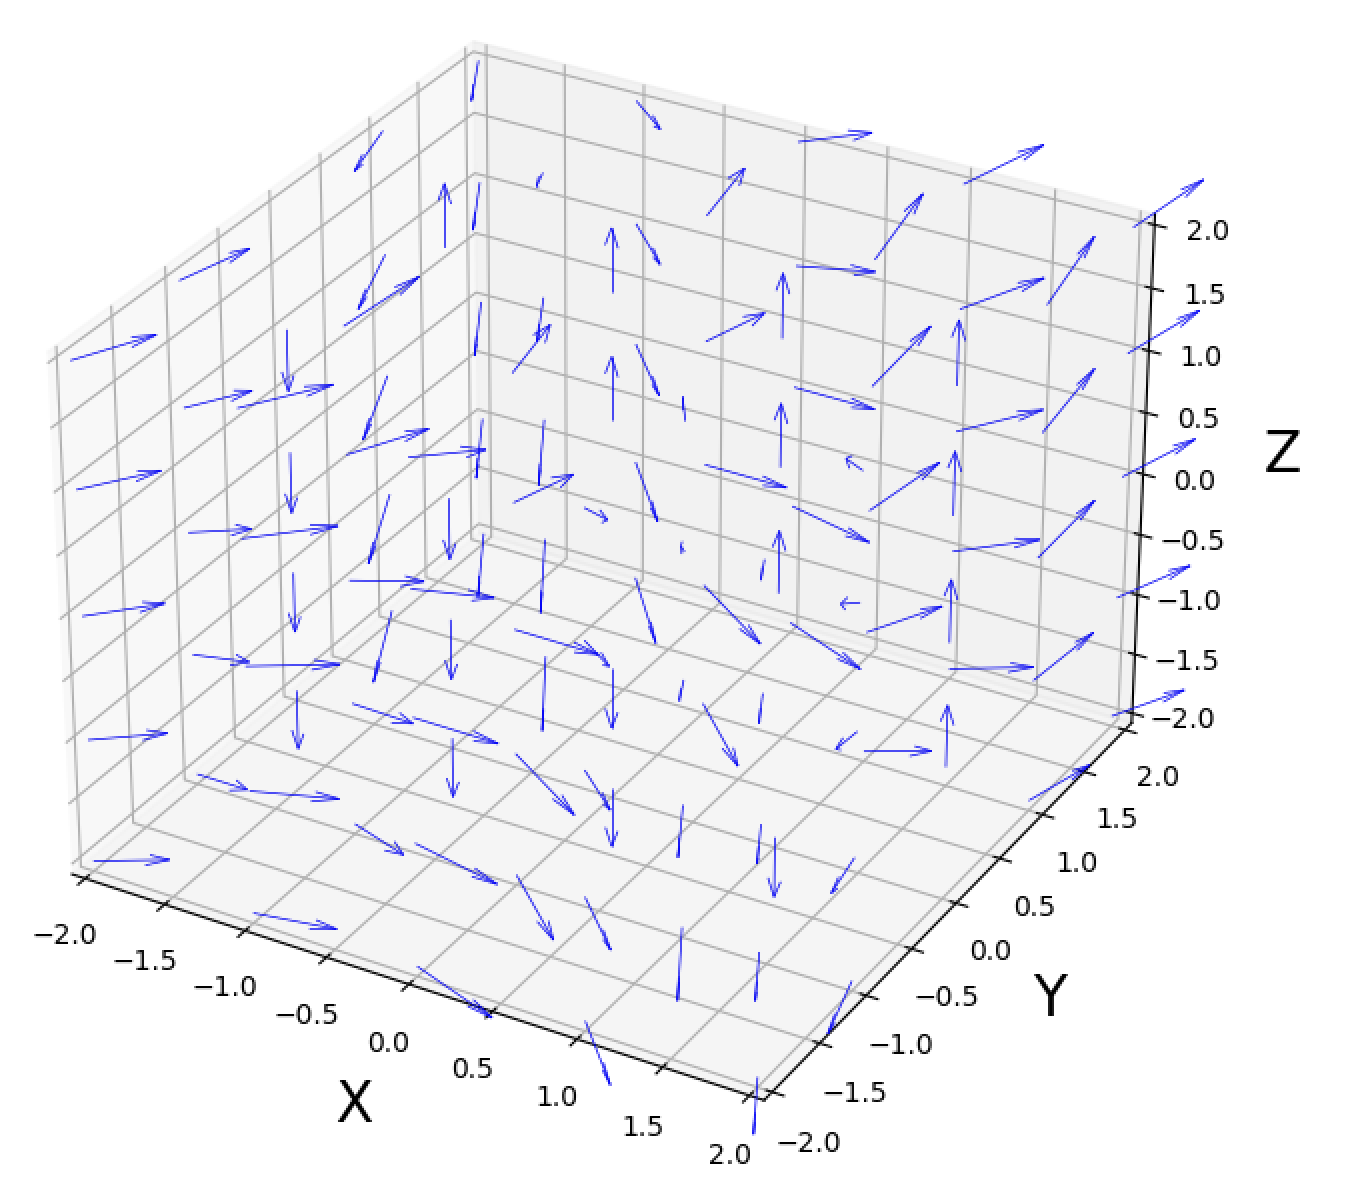
\includegraphics[width=\textwidth]{chapters/chp5_pics/5.2.4.png}
        \caption{}
        \label{fig:3d_vec_field}
    \end{subfigure}
    \caption{The path of the curves (a) with the 3D vector field plotted separately using Python (b)}
    \label{fig:comparison}
\end{figure}

\begin{solution} We'll evaluate the line integral along each segment and sum the results:
\[
\int_C \mathbf{F}\cdot d\mathbf{r} = \int_{C_1} \mathbf{F}\cdot d\mathbf{r} + \int_{C_2} \mathbf{F}\cdot d\mathbf{r} + \int_{C_3} \mathbf{F}\cdot d\mathbf{r}
\]
\noindent We will also make use of 

\[
\int_C \mathbf{F} \cdot d\mathbf{r} =  \int_a^b \left[P\frac{dx}{dt} + Q\frac{dy}{dt} + R\frac{dz}{dt}\right]\,dt.
\]

\begin{enumerate}

\item Along $C_1$ (from $A$ to $B$):
\begin{itemize}
    \item Parameterization: $\mathbf{r}(t) = t\mathbf{i} + 0\mathbf{j} + 0\mathbf{k}$, $0 \leq t \leq 1$
    \item $\frac{d\mathbf{r}}{dt} = \mathbf{i}$
    \item Along this path: $y=0$, $z=0$, and $x=t$
    \item Plug into $\mathbf{F} = (y^2)\mathbf{i} + (2xy)\mathbf{j} + (x+z)\mathbf{k}$ to get $\mathbf{F}(\mathbf{r}(t)) = (0)\mathbf{i} + (0)\mathbf{j} + (t)\mathbf{k}$
\end{itemize}
Therefore:
\begin{align*}
\int_{C_1} \mathbf{F}\cdot d\mathbf{r} &= \int_0^1 [(0)(1) + (0)(0) + (t)(0)]\,dt = 0
\end{align*}

\item Along $C_2$ (from $B$ to $C$):
\begin{itemize}
    \item Parameterization: $\mathbf{r}(t) = 1\mathbf{i} + t\mathbf{j} + 0\mathbf{k}$, $0 \leq t \leq 1$
    \item $\frac{d\mathbf{r}}{dt} = \mathbf{j}$
    \item Along this path: $x=1$, $z=0$, and $y=t$
    \item Plug into $\mathbf{F} = (y^2)\mathbf{i} + (2xy)\mathbf{j} + (x+z)\mathbf{k}$ to get $\mathbf{F}(\mathbf{r}(t)) = (t^2)\mathbf{i} + (2t)\mathbf{j} + (1)\mathbf{k}$
\end{itemize}
Therefore:
\begin{align*}
\int_{C_2} \mathbf{F}\cdot d\mathbf{r} &= \int_0^1 [(t^2)(0) + (2t)(1) + (1)(0)]\,dt \\
&= \int_0^1 2t\,dt = [t^2]_0^1 = 1
\end{align*}

\item Along $C_3$ (from $C$ to $D$):
\begin{itemize}
    \item Parameterization: $\mathbf{r}(t) = 1\mathbf{i} + 1\mathbf{j} + t\mathbf{k}$, $0 \leq t \leq 1$
    \item $\frac{d\mathbf{r}}{dt} = \mathbf{k}$
    \item Along this path: $x=1$, $y=1$, and $z=t$
    \item Plug into $\mathbf{F} = (y^2)\mathbf{i} + (2xy)\mathbf{j} + (x+z)\mathbf{k}$ to get $\mathbf{F}(\mathbf{r}(t)) = (1)\mathbf{i} + (2)(1)\mathbf{j} + (1+t)\mathbf{k}$
\end{itemize}
Therefore:
\begin{align*}
\int_{C_3} \mathbf{F}\cdot d\mathbf{r} &= \int_0^1 [(1)(0) + (2)(0) + (1+t)(1)]\,dt \\
&= \int_0^1 (1+t)\,dt = [t + \frac{t^2}{2}]_0^1 = \frac{3}{2}
\end{align*}
\end{enumerate}

The total line integral is:
\[
\int_C \mathbf{F}\cdot d\mathbf{r} = 0 + 1 + \frac{3}{2} = \frac{5}{2}
\]
\end{solution}
\end{example}
\exampleline

\subsection*{Potential Functions and Conservative Fields}

\noindent Let's now explore a special class of vector fields that yield remarkable properties. Consider a vector field $\mathbf{F}(x,y)$ defined on a simply connected domain $D$. A vector field is conservative if it can be written as the gradient of some scalar function $f(x,y)$:
\[
\mathbf{F}(x,y) = \nabla f = \frac{\partial f}{\partial x}\mathbf{i} + \frac{\partial f}{\partial y}\mathbf{j}
\]

\noindent This means that $P(x,y) = \frac{\partial f}{\partial x}$ and $Q(x,y) = \frac{\partial f}{\partial y}$. The requirement of a simply connected domain is crucial here—it ensures that any closed path can be continuously deformed to a point, which will prove essential for the path independence of our line integrals. Let's see what happens when we compute a line integral in such a field. Consider a curve $C$ lying entirely in $D$ and parameterized by $\mathbf{r}(t) = x(t)\mathbf{i} + y(t)\mathbf{j}$ from $t=a$ to $t=b$. \\

\noindent Starting with the vector field line integral:
\begin{align*}
\int_C \mathbf{F} \cdot d\mathbf{r} &= \int_C P(x,y)\,dx + Q(x,y)\,dy \\
&= \int_a^b \left[P(x(t),y(t))\frac{dx}{dt} + Q(x(t),y(t))\frac{dy}{dt}\right]\,dt
\end{align*}

\noindent Now, because $\mathbf{F}$ is conservative on our simply connected domain $D$, we can substitute $P = \frac{\partial f}{\partial x}$ and $Q = \frac{\partial f}{\partial y}$:
\begin{align*}
\int_C \mathbf{F} \cdot d\mathbf{r} &= \int_a^b \left[\frac{\partial f}{\partial x}\frac{dx}{dt} + \frac{\partial f}{\partial y}\frac{dy}{dt}\right]\,dt
\end{align*}

\noindent The key insight is recognizing that this is the chain rule for the total derivative of $f$ with respect to $t$:
\begin{align*}
\int_C \mathbf{F} \cdot d\mathbf{r} &= \int_a^b \frac{d}{dt}[f(x(t),y(t))]\,dt \\
&= f(x(b),y(b)) - f(x(a),y(a)) \\
&= f(B) - f(A)
\end{align*}

\noindent This derivation reveals the Fundamental Theorem of Line Integrals: \index{Fundamental Theorem of Line Integrals}
\[
\int_C \mathbf{F} \cdot d\mathbf{r} = f(B) - f(A)
\]
\noindent Note that this result, valid on our simply connected domain $D$, demonstrates that the line integral depends only on the endpoints $A$ and $B$, not on the particular path chosen—a powerful consequence of both the conservative nature of $\mathbf{F}$ and the simple connectivity of $D$. This looks remarkably similar to our good old friend, the Fundamental Theorem of Calculus II. \\

\noindent To build some physical intuition, think of climbing a mountain. The work (force $\times$ displacement) done against gravity (a conservative field) depends only on your starting and ending elevations, not the path you take—whether you climb straight up or take a winding trail. The simple connectivity of the domain ensures there are no ``holes" in the mountain that would force you to take fundamentally different paths (imagine if there were a bottomless pit you had to walk around). Meanwhile, the conservative nature of the field ensures that no energy is gained or lost in cycles—if you end where you started, the total work is zero, just as walking around the mountain at the same elevation requires no net work against gravity. \\

\noindent The importance of simply connected domains becomes even more profound when we delve into complex integration in Chapter 7. There, this concept forms the foundation of Cauchy's Integral Theorem and leads to the remarkable theory of complex analytic functions, where the implications of path independence reach far deeper than in the real case.

\begin{figure}[H]
    \centering
    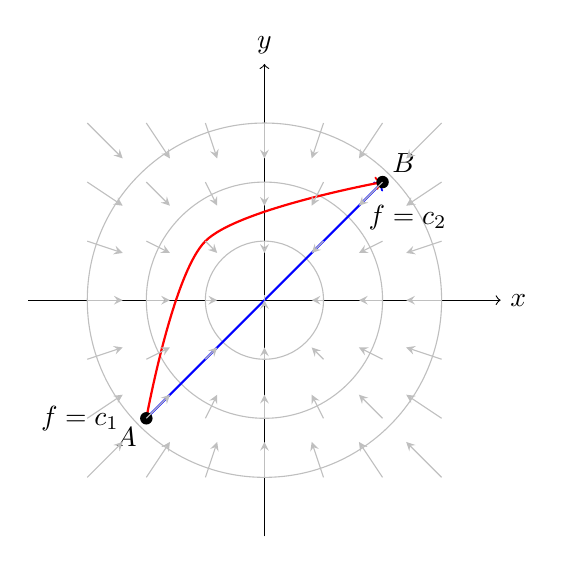
\begin{tikzpicture}[scale=1.5]
        % Axes
        \draw[->] (-2,0) -- (2,0) node[right] {$x$};
        \draw[->] (0,-2) -- (0,2) node[above] {$y$};
        
        % Draw level curves
        \foreach \r in {0.5,1,1.5} {
            \draw[gray!50] (0,0) circle (\r);
        }
        
        % Draw two different paths
        \draw[blue, thick, ->] (-1,-1) -- (1,1);
        \draw[red, thick, ->] plot[smooth] coordinates {(-1,-1) (-0.5,0.5) (1,1)};
        
        % Add points and labels
        \fill (-1,-1) circle (1.5pt) node[below left] {$A$};
        \fill (1,1) circle (1.5pt) node[above right] {$B$};
        
        % Add potential function values
        \node[left] at (-1.15,-1) {$f=c_1$};
        \node[right] at (0.8,0.7) {$f=c_2$};
        
        % Add field vectors (with fixed spacing to avoid computation issues)
        \foreach \x in {-1.5,-1,-0.5,0,0.5,1,1.5} {
            \foreach \y in {-1.5,-1,-0.5,0,0.5,1,1.5} {
                \draw[-stealth, gray!50, thin] (\x,\y) -- +({-\x/5},{-\y/5});
            }
        }
    \end{tikzpicture}
    \caption{\textit{In a conservative field, the line integral equals the change in potential function value, regardless of path taken. Level curves of $f$ (gray circles) are perpendicular to the field vectors.}}
    \label{fig:potential_function}
    \end{figure}

\noindent This powerful result has several profound implications:

\begin{enumerate}
\item \textbf{Path Independence:} On a simply connected domain, a vector field $\mathbf{F}$ is path-independent if and only if it's conservative, meaning the line integral depends only on the endpoints $A$ and $B$, not on the path taken between them. This is because we're simply measuring the total change in the potential function $f$. Remember to check for the conservation by comparing all combinations of the partial derivatives. For a vector field in $n$ dimensions with components $F_1, F_2, ..., F_n$:
\[
\frac{\partial F_i}{\partial x_j} = \frac{\partial F_j}{\partial x_i} \quad \text{for all } i,j \in \{1,...,n\}, \, i \neq j
\]
For example, in three dimensions ($n=3$ dimensions), this gives us:
\[
\frac{\partial P}{\partial y} = \frac{\partial Q}{\partial x}, \quad
\frac{\partial P}{\partial z} = \frac{\partial R}{\partial x}, \quad
\frac{\partial Q}{\partial z} = \frac{\partial R}{\partial y}
\]

    \item \textbf{Closed Paths:} If $C$ is a closed path (where $A=B$), then:
    \[
    \oint_C \mathbf{F} \cdot d\mathbf{r} = f(A) - f(A) = 0
    \]
    The circle in the integral symbol reminds us we're integrating around a closed loop.
    
    \item \textbf{Equipotential Curves:} Along any curve where $f$ is constant (level curves of $f$), the line integral is zero because there's no change in potential.
\end{enumerate}

\noindent In physics, this theorem explains why conservative forces (like gravity) do work that depends only on initial and final positions, not the path taken. The potential function $f$ might represent Gravitational potential energy, Electric potential in an electrostatic field, Pressure potential in a static fluid, and more. \\

\noindent This connection between conservative vector fields and potential functions provides both computational simplification and deep physical insight. When we can identify a potential function, complicated line integral calculations reduce to simple evaluation at endpoints. \\

\noindent Let's take some examples of these concepts now:

\exampleline
\begin{example}
For each of the following vector fields:
\begin{itemize}
    \item Check if the field is conservative
    \item If conservative, find its potential function
    \item Evaluate the given line integral
\end{itemize}
\noindent Vector fields and regions:

\begin{enumerate}
\item $\mathbf{F}_1(x,y) = (3x^2 + y)\mathbf{i} + (x + 4y^3)\mathbf{j}$ on $\mathbb{R}^2$\\
Evaluate $\oint_C \mathbf{F}_1\cdot d\mathbf{r}$ along the closed curve $C$ shown:

\begin{center}
\begin{tikzpicture}[scale=1]
    % Draw axes
    \draw[->] (-2,0) -- (4,0) node[right] {$x$};
    \draw[->] (0,-1) -- (0,2.2) node[above] {$y$};
    
    % Draw a closed curve (ellipse)
    \draw[thick, blue] plot [smooth cycle, tension=1] coordinates { 
        (-1,1) (1,2) (3,1) (1,0) 
    };
    
    % Label the curve
    \node at (2.3,1.3) {$C$};
\end{tikzpicture}
\end{center}

\item $\mathbf{F}_2(x,y) = e^y\mathbf{i} + xe^y\mathbf{j}$ on $\mathbb{R}^2$\\
Evaluate $\int_C \mathbf{F}_2\cdot d\mathbf{r}$ from $A(0,0)$ to $B(1,2)$ along the curve shown:

\begin{center}
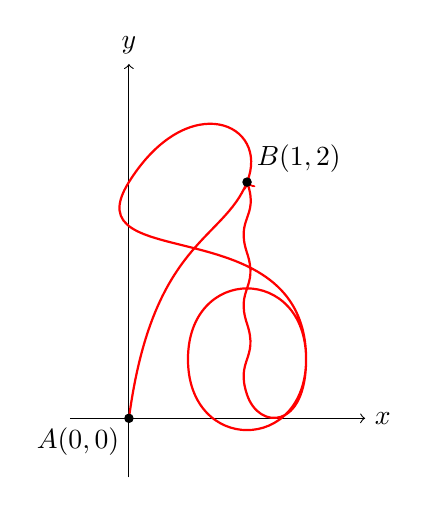
\begin{tikzpicture}[scale=1.5]
% Draw axes
\draw[->] (-0.5,0) -- (2,0) node[right] {$x$};
\draw[->] (0,-0.5) -- (0,3) node[above] {$y$};
% Draw a wild line
\draw[thick, red, ->] (0,0) .. controls (0.2,1.5) and (0.8,1.5) .. (1,2)
.. controls (1.2,2.5) and (0.5,2.8) .. (0,2)
.. controls (-0.5,1.2) and (1.5,1.8) .. (1.5,0.5)
.. controls (1.5,-0.3) and (0.5,-0.3) .. (0.5,0.5)
.. controls (0.5,1.3) and (1.5,1.3) .. (1.5,0.5)
.. controls (1.5,-0.1) and (1.1,-0.1) .. (1,0.2)
.. controls (0.9,0.5) and (1.1,0.5) .. (1,0.8)
.. controls (0.9,1.1) and (1.1,1.1) .. (1,1.4)
.. controls (0.9,1.7) and (1.1,1.7) .. (1,2);
% Label points A and B
\filldraw [black] (0,0) circle (1pt) node[anchor=north east] {$A(0,0)$};
\filldraw [black] (1,2) circle (1pt) node[anchor=south west] {$B(1,2)$};
\end{tikzpicture}
\end{center}

\item $\mathbf{F}_3(x,y) = \frac{-y}{x^2 + y^2}\mathbf{i} + \frac{x}{x^2 + y^2}\mathbf{j}$ on $\mathbb{R}^2\setminus\{(0,0)\}$\\
Evaluate $\oint_C \mathbf{F}_3\cdot d\mathbf{r}$ along any circle centered at the origin.
\end{enumerate}

\begin{solution}
\begin{enumerate}
\item For $\mathbf{F}_1$:
    \begin{itemize}
        \item Check if conservative by comparing partial derivatives:
        \[
        \frac{\partial P}{\partial y} = 1 = \frac{\partial Q}{\partial x}
        \]
        \item Since these are equal and the domain is simply connected, $\mathbf{F}_1$ is conservative
        \item Find potential function by integrating $P$ with respect to $x$:
        \begin{align*}
        f(x,y) &= \int (3x^2 + y)\,dx = x^3 + xy + g(y) \\
        \frac{\partial f}{\partial y} &= x + g'(y) = x + 4y^3 \quad \text{(comparing with $Q$)} \\
        g(y) &= y^4 + C
        \end{align*}
        \item Therefore, $f(x,y) = x^3 + xy + y^4 + C$
        \item For any closed curve over a conservative vector: $\oint_C \mathbf{F}_1\cdot d\mathbf{r} = 0$
    \end{itemize}

    \item For $\mathbf{F}_2$:
    \begin{itemize}
        \item Check partial derivatives:
        \[
        \frac{\partial P}{\partial y} = e^y = \frac{\partial Q}{\partial x}
        \]
        \item Field is conservative on $\mathbb{R}^2$ (simply connected domain)
        \item Find potential function:
        \begin{align*}
        f(x,y) &= \int e^y\,dx = xe^y + g(y) \\
        \frac{\partial f}{\partial y} &= xe^y + g'(y) = xe^y \quad \text{(comparing with $Q$)} \\
        g(y) &= C
        \end{align*}
        \item Therefore, $f(x,y) = xe^y + C$
        \item Line integral from $A(0,0)$ to $B(1,2)$:
        \begin{align*}
        \int_C \mathbf{F}_2\cdot d\mathbf{r} &= f(B) - f(A) \\
        &= [f(1,2)] - [f(0,0)] \\
        &= [(1)e^2 + C] - [(0)e^0 + C] \\
        &= e^2 + C - C \\
        &= e^2
        \end{align*}
        Note how the constant $C$ cancels in the difference.
    \end{itemize}


    \item For $\mathbf{F}_3$:
    \begin{itemize}
        \item Check partial derivatives:
        \begin{align*}
        \frac{\partial P}{\partial y} &= \frac{-x^2 + y^2}{(x^2 + y^2)^2} \\
        \frac{\partial Q}{\partial x} &= \frac{-x^2 + y^2}{(x^2 + y^2)^2}
        \end{align*}
        \item Although partial derivatives are equal, domain is not simply connected (origin removed)
        \item Therefore $\mathbf{F}_3$ is not conservative
        \item For a circle of radius $r$ centered at origin, parameterize on $t \in [0,2\pi]$ using:
        \[
        x = r\cos\theta, \quad y = r\sin\theta
        \]
        \item Calculating $\mathbf{F}_3 \cdot d\mathbf{r}$:
        \begin{align*}
            \mathbf{F}_3 &= \frac{-y}{r^2}\mathbf{i} + \frac{x}{r^2}\mathbf{j} = \frac{-\sin\theta}{r}\mathbf{i} + \frac{\cos\theta}{r}\mathbf{j} \\
            d\mathbf{r} &= \frac{dx}{d\theta}d\theta\mathbf{i} + \frac{dy}{d\theta}d\theta\mathbf{j} = -r\sin\theta d\theta\mathbf{i} + r\cos\theta d\theta\mathbf{j}
        \end{align*}
        \item Taking the dot product:
        \begin{align*}
            \mathbf{F}_3 \cdot d\mathbf{r} &= \left(\frac{-\sin\theta}{r}\right)(-r\sin\theta d\theta) + \left(\frac{\cos\theta}{r}\right)(r\cos\theta d\theta) \\
            &= \sin^2\theta d\theta + \cos^2\theta d\theta \\
            &= (\sin^2\theta + \cos^2\theta)d\theta = d\theta
        \end{align*}
        \item Therefore, for any circle centered at origin:
        \[
        \oint_C \mathbf{F}_3\cdot d\mathbf{r} = \int_0^{2\pi} 1\,d\theta = 2\pi
        \]
        regardless of the radius $r$
    \end{itemize}

\end{enumerate}
\end{solution}
\end{example}
\exampleline

\exampleline
\begin{example}
Show that \( \mathbf{F}(x,y,z) = \langle yz, \, xz, \, xy \rangle \) is conservative and find a potential function.

\begin{solution}
We check: \( \partial P/\partial y = z = \partial Q/\partial x \), \( \partial P/\partial z = y = \partial R/\partial x \), \( \partial Q/\partial z = x = \partial R/\partial y \). All conditions are satisfied, so \( \mathbf{F} \) is conservative.\\ \\
\noindent To find \( f \), integrate \( P = yz \) with respect to \( x \):
\[ f(x,y,z) = xyz + g(y,z). \]
Differentiate with respect to \( y \): \( f_y = xz + g_y(y,z) \). Setting this equal to \( Q = xz \) gives \( g_y = 0 \), so \( g(y,z) = h(z) \).\\ \\
\noindent Differentiate with respect to \( z \): \( f_z = xy + h'(z) \). Setting this equal to \( R = xy \) gives \( h'(z) = 0 \), so \( h(z) = C \).\\ \\
\noindent Therefore \( f(x,y,z) = xyz + C \).
\end{solution}
\end{example}
\exampleline


\newpage

\lecture{Green's Theorem} \index{Green's Theorem} \index{Flux}

\noindent The relationship between derivatives and integrals stands as one of the most profound insights in mathematics. We've seen this connection in various forms: the Fundamental Theorem of Calculus linking derivatives to single integrals, and the relationship between partial derivatives and multiple integrals in higher dimensions. Now we explore another manifestation of this deep connection—Green's Theorem—which relates line integrals around a closed curve to double integrals over the region it encloses. This relationship not only provides computational power but also reveals fundamental properties of vector fields and their behavior in the plane. \\

\noindent The path to understanding Green's Theorem will leverage several powerful tools from our mathematical arsenal. The Mean Value Theorem will help us analyze vector field behavior over small intervals, while Taylor's Theorem will allow us to approximate vector components with increasing accuracy. These classical results, combined with careful limiting arguments, will reveal how local vector field properties accumulate to create global patterns of circulation and flux, which refers to the flow of the vector field through a surface. \\

\noindent Our journey begins with an intuitive understanding through fluid flow, moves through rigorous mathematical development, and culminates in a theorem that bridges boundary behavior with interior properties. Just as the Fundamental Theorem of Calculus shows how differentiation and integration are inverse processes, Green's Theorem will demonstrate how boundary circulation captures the cumulative effect of interior rotation. This lecture represents an important leap in mathematical formalism for advanced theorems that you may not have encountered before. Don't get caught up too much in the detail, but stop to appreciate how we lay out the architecture. 


\subsection*{Motivation and Mathematical Foundation}

\noindent Before diving into the mathematics, let's build some intuition. Imagine a lake with a current described by a vector field $\mathbf{F}(x,y) = P(x,y)\mathbf{i} + Q(x,y)\mathbf{j}$. When studying this flow, we might be interested in two fundamental quantities:

\begin{itemize}
    \item The circulation of the water around the lake's boundary
    \item How much the water rotates or ``swirls" at each point inside the lake
\end{itemize}

\noindent The first quantity measures boundary behavior through a line integral $\oint_C \mathbf{F}\cdot d\mathbf{r}$, while the second examines interior rotation through derivatives $\frac{\partial Q}{\partial x} - \frac{\partial P}{\partial y}$. Green's Theorem reveals that these seemingly different measurements are intimately connected—the total circulation around the boundary exactly equals the sum of all the interior rotation. \\

\noindent To understand Green's Theorem from a rigorous mathematical perspective, let's begin to build the framework piece by piece using tools we know. Consider a simple closed curve $C$ with four constituent parts $C_1,...,C_4$ in the plane, oriented counterclockwise, that bounds a region $D$. We can think about this curve in two complementary ways:

\begin{enumerate}
    \item As the boundary where we might evaluate a line integral
    \item As the edge of a region where we might compute a double integral
\end{enumerate}

\begin{figure}[H]
\centering
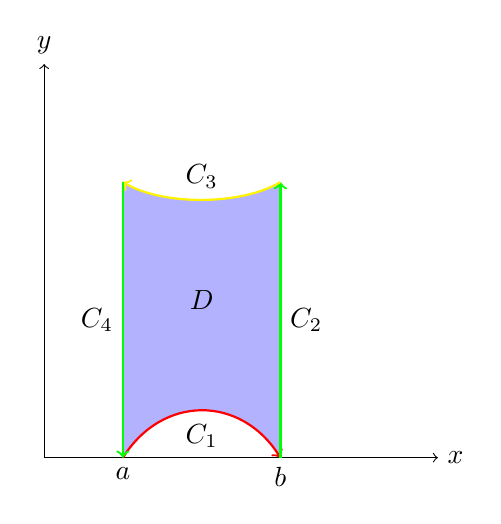
\begin{tikzpicture}
    % Draw axes
    \draw[->] (0,0) -- (5,0) node[right] {$x$};
    \draw[->] (0,0) -- (0,5) node[above] {$y$};
    
    % Draw region D with modified boundary
    \begin{scope}
        \clip (0.8,0) rectangle (3.2,4);
        \fill[blue!30] (1,0) .. controls (1.5,0.8) and (2.5,0.8) .. (3,0)  % C₁
            -- (3,3.5) % C₂
            .. controls (2.5,3.2) and (1.5,3.2) .. (1,3.5) % C₃
            -- (1,0); % C₄
    \end{scope}
    
    % Draw colored boundary segments with arrows for counterclockwise direction
    \draw[red, thick, ->] (1,0) .. controls (1.5,0.8) and (2.5,0.8) .. (3,0);    % C₁
    \draw[green, thick, ->] (3,0) -- (3,3.5);  % C₂
    \draw[yellow, thick, ->] (3,3.5) .. controls (2.5,3.2) and (1.5,3.2) .. (1,3.5); % C₃
    \draw[green, thick, ->] (1,3.5) -- (1,0);  % C₄
    
    % Add labels
    \node at (2,2) {$D$};
    \node[below] at (1,0) {$a$};
    \node[below] at (3,0) {$b$};
    \node[below] at (2,0.55) {$C_1$};
    \node[right] at (3,1.75) {$C_2$};
    \node[above] at (2,3.3) {$C_3$};
    \node[left] at (1,1.75) {$C_4$};
\end{tikzpicture}

\caption{\textit{A region $D$ bounded by a curve $C = C_1 + C_2 + C_3 + C_4$. We can begin to heuristically see the relationship between the line integral and the double integral.}}
\label{fig:green}
\end{figure}

\noindent Let's explore why these perspectives might be related. Consider breaking our region into tiny rectangles with sides $\Delta x$ and $\Delta y$. For each rectangle:

\begin{itemize}
    \item The line integral around its boundary involves terms like $P\Delta x$ and $Q\Delta y$
    \item The double integral over its area involves terms like $\frac{\partial Q}{\partial x}\Delta x\Delta y$ and $\frac{\partial P}{\partial y}\Delta x\Delta y$
\end{itemize}

\noindent This suggests a possible connection between:
\[
\text{Boundary Terms: } P\Delta x + Q\Delta y 
\]
and
\[
\text{Area Terms: } \left(\frac{\partial Q}{\partial x} - \frac{\partial P}{\partial y}\right)\Delta x\Delta y
\]

\begin{figure}[H]
\centering

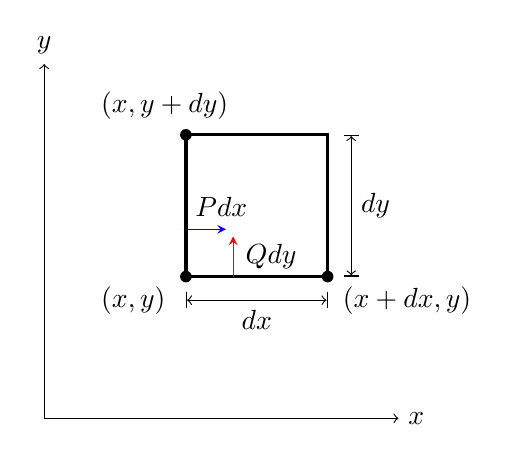
\begin{tikzpicture}[scale=3]
    % Draw main axes
    \draw[->] (0,0) -- (1.5,0) node[right] {$x$};
    \draw[->] (0,0) -- (0,1.5) node[above] {$y$};

    % Draw rectangle (differential element)
    \draw[very thick] (0.6,0.6) rectangle (1.2,1.2);

    % Add dots at vertices
    \fill (0.6,0.6) circle (0.7pt);  % (x,y)
    \fill (1.2,0.6) circle (0.7pt);  % (x+dx,y)
    \fill (0.6,1.2) circle (0.7pt);  % (x,y+dy)

    % Label vertices
    \node[below right] at (0.2,0.6) {$(x,y)$};
    \node[below right, xshift=2] at (1.2,0.6) {$(x+dx,y)$};
    \node[above right, yshift=2] at (0.2,1.2) {$(x,y+dy)$};

    % Add vector field components with arrows and separate labels
    \draw[-stealth, red] (0.8,0.6) -- (0.8,0.77);
    \node[right, xshift=1] at (0.8,0.685) {$Qdy$};
    
\draw[-stealth, blue] (0.6,0.8) -- (0.77,0.8);
    \node[above, yshift=1] at (0.75,0.8) {$Pdx$};

    % Label differential measurements
    \draw[|<->|] (0.6,0.5) -- (1.2,0.5) node[midway,below] {$dx$};
    \draw[|<->|] (1.3,0.6) -- (1.3,1.2) node[midway,right] {$dy$};
\end{tikzpicture}
\caption{\textit{Differential element showing contributions of a vector field $(P,Q)$ to the line integral around the boundary of the rectangular area element $dxdy$.}}
\label{fig:differential_element}
\end{figure}

\noindent To formalize this intuition, let's examine what happens when we sum the line integral contributions around a single small rectangle with vertices at $(x,y)$, $(x+\Delta x,y)$, $(x+\Delta x,y+\Delta y)$, and $(x,y+\Delta y)$:

\begin{align*}
\oint_{\text{rect}} P\,dx + Q\,dy &= \int_{x}^{x+\Delta x} P(s,y)\,ds + \int_{y}^{y+\Delta y} Q(x+\Delta x,t)\,dt \\
&\quad - \int_{x+\Delta x}^{x} P(s,y+\Delta y)\,ds - \int_{y+\Delta y}^{y} Q(x,t)\,dt.
\end{align*}

\noindent Using the Mean Value Theorem and Taylor's Theorem, we expand $Q(x+\Delta x, y)$ and $P(x, y+\Delta y)$ around $(x, y)$:

\begin{align*}
Q(x+\Delta x,y) &= Q(x,y) + \frac{\partial Q}{\partial x}\Delta x + O(\Delta x^2), \\
P(x,y+\Delta y) &= P(x,y) + \frac{\partial P}{\partial y}\Delta y + O(\Delta y^2).
\end{align*}

\noindent For higher-order terms ($O(\Delta x^2)$, for example), note that these terms vanish in the limit as $\Delta x, \Delta y \to 0$ due to their smaller magnitude compared to $\Delta x$ or $\Delta y$. After careful algebraic manipulation, the line integral around the rectangle simplifies to:

\[
\oint_{\text{rect}} P\,dx + Q\,dy = \left(\frac{\partial Q}{\partial x} - \frac{\partial P}{\partial y}\right)\Delta x\Delta y + O(\Delta x^2\Delta y + \Delta x\Delta y^2).
\]

\noindent Here, $\Delta x\Delta y$ represents the leading-order contribution proportional to the area of the rectangle, while the higher-order terms vanish faster than $\Delta x\Delta y$ as $\Delta x, \Delta y \to 0$. This dominant term transitions to the differential $dx\,dy$ in the integral when taking the limit over all rectangles.

\bigskip

\noindent The key insight is this: if we partition the entire region $D$ into such small rectangles and sum their contributions, the following occurs:

\begin{itemize}
    \item Interior edges cancel in pairs, as they are traversed in opposite directions.
    \item Only the boundary edges survive, forming the boundary $\partial D$ of the region $D$.
    \item The sum of area terms provides an approximation to the double integral over $D$.
\end{itemize}

\bigskip

\noindent Taking the limit as the partition becomes infinitely fine, let the partition consist of $n$ rectangles, each with area $\Delta A_i = \Delta x_i\Delta y_i$. For each rectangle $R_i$, the local line integral can be expressed as:

\[
\oint_{\partial R_i} P\,dx + Q\,dy = \left(\frac{\partial Q}{\partial x} - \frac{\partial P}{\partial y}\right)\Delta A_i + O(\Delta x_i^2\Delta y_i + \Delta x_i\Delta y_i^2).
\]

\noindent Summing over all rectangles, we obtain:

\begin{align*}
\sum_{i=1}^n \oint_{\partial R_i} P\,dx + Q\,dy &= \sum_{i=1}^n \left[\left(\frac{\partial Q}{\partial x} - \frac{\partial P}{\partial y}\right)\Delta A_i + O(\Delta x_i^2\Delta y_i + \Delta x_i\Delta y_i^2)\right] \\[1em]
&= \sum_{i=1}^n \left(\frac{\partial Q}{\partial x} - \frac{\partial P}{\partial y}\right)\Delta A_i + \sum_{i=1}^n O(\Delta x_i^2\Delta y_i + \Delta x_i\Delta y_i^2).
\end{align*}

\noindent Let $\delta = \max_i\{\Delta x_i, \Delta y_i\}$ denote the mesh size of the partition. The error term is then bounded by:
\[
\left|\sum_{i=1}^n O(\Delta x_i^2\Delta y_i + \Delta x_i\Delta y_i^2)\right| \leq M\delta \text{Area}(D),
\]
for some constant $M$. As $\delta \to 0$, the error term vanishes, leaving:
\[
\lim_{\delta \to 0} \sum_{i=1}^n \oint_{\partial R_i} P\,dx + Q\,dy = \lim_{\delta \to 0} \sum_{i=1}^n \left(\frac{\partial Q}{\partial x} - \frac{\partial P}{\partial y}\right)\Delta A_i.
\]

\noindent On the left-hand side, the sum of line integrals reduces to the line integral around the boundary of the region:
\[
\oint_{\partial D} P\,dx + Q\,dy.
\]
On the right-hand side, the Riemann sum transitions to the double integral over $D$:
\[
\lim_{\delta \to 0} \sum_{i=1}^n \left(\frac{\partial Q}{\partial x} - \frac{\partial P}{\partial y}\right)\Delta A_i = \iint_D \left(\frac{\partial Q}{\partial x} - \frac{\partial P}{\partial y}\right)\,dA.
\]

\bigskip

\noindent Through this limiting process, the local relationships derived for small rectangles extend to the entire region $D$. As the partition becomes infinitely fine ($\delta \to 0$), the sum of approximations converges to exact values: the line integral around the boundary of $D$ is precisely balanced by the double integral of the curl over the region. This establishes \textbf{Green's Theorem}:
\[
\oint_{\partial D} \mathbf{F} \cdot d\mathbf{r} = \oint_{\partial D} P\,dx + Q\,dy = \iint_D \left(\frac{\partial Q}{\partial x} - \frac{\partial P}{\partial y}\right)\,dA.
\]
\noindent Here \( \partial D \) is traversed counterclockwise (positive orientation), and \( D \) must be simply connected.\\ \\

\noindent Green's Theorem also has a \textit{flux form}. If \( \mathbf{F} = P\mathbf{i} + Q\mathbf{j} \), then:
\[
\oint_{\partial D} (P \, dy - Q \, dx) = \iint_D \left(\frac{\partial P}{\partial x} + \frac{\partial Q}{\partial y}\right) dA = \iint_D \operatorname{div} \mathbf{F} \, dA.
\]
The circulation form generalizes to Stokes' Theorem; the flux form generalizes to the Divergence Theorem.\\ \\
\noindent A useful consequence of Green's Theorem is the \textbf{area formula}:
\[
A = \frac{1}{2}\oint_C (x \, dy - y \, dx),
\]
which computes the area of the region enclosed by a simple closed curve \( C \).\\ \\
\noindent This theorem stands as a fundamental bridge between different types of integration, much like how the Fundamental Theorem of Calculus I connects derivatives and integrals in single-variable calculus. What makes this theorem even more remarkable is that it solves so many physics problems with surprisingly few physical assumptions. As the saying goes, the potency of a law is the strength of what it proves divided by what it assumes. \\

\noindent We can now substitute line integrals for double integrals wherever it proves advantageous—a frequent and powerful simplification! Do you see anything interesting about the integrand? Anything that connects to Chapter 1 vector concepts? We will soon make an important generalization of Green's Theorem, but as an exercise, try to see if you can adjust this formula for any dimension $n$. \\

\noindent Let's consider one more intuitive example. Imagine a region enclosed by a smooth, oriented curve $C$, as shown in the diagram. Inside this curve, we have several small, uniformly distributed loops, all oriented in the same direction. Each of these loops can be thought of as representing a local rotational field or a ``microscopic circulation" at each point in the region. The arrows on the boundary $C$ indicate the macroscopic circulation along the curve's orientation. By Green's Theorem, the total circulation along $C$ is equal to the sum of these individual microscopic rotations, effectively connecting the behavior of the field inside the region to its boundary.


\exampleline
\begin{example}
Consider the vector field $\mathbf{F}(x,y) = (x^3y^2)\mathbf{i} + (x^2y^3)\mathbf{j}$. Evaluate $\oint_C \mathbf{F}\cdot d\mathbf{r}$, where $C$ is the triangle with vertices at $(0,0)$, $(1,0)$, and $(0,1)$, oriented counterclockwise.

\begin{solution}
We'll solve this two ways: first directly using the line integral, and then using Green's Theorem.

\begin{enumerate}
\item \textbf{Method 1: Direct Line Integral}

Split the boundary \(C\) into three segments: 
\begin{itemize}
    \item \(C_1\): From \((0,0)\) to \((1,0)\),
    \item \(C_2\): From \((1,0)\) to \((0,1)\),
    \item \(C_3\): From \((0,1)\) to \((0,0)\).
\end{itemize}
Let's crunch these now (even though if you look at the vector field you may already know the answer...)
\begin{enumerate}
\item \(C_1\): From \((0,0)\) to \((1,0)\)
Parameterize \(C_1\):
\[
\mathbf{r}_1(t) = (t, 0), \quad 0 \leq t \leq 1, \quad \text{so } \frac{d\mathbf{r}_1}{dt} = (1, 0).
\]
Evaluate \(\mathbf{F} \cdot d\mathbf{r}\) along \(C_1\):
\[
\mathbf{F}(x,y) = (x^3y^2, x^2y^3), \quad \mathbf{F}(\mathbf{r}_1(t)) = (t^3 \cdot 0^2, t^2 \cdot 0^3) = (0, 0).
\]
Thus:
\[
\int_{C_1} \mathbf{F} \cdot d\mathbf{r} = \int_0^1 (0)(1) + (0)(0)\,dt = 0.
\]

\item \(C_2\): From \((1,0)\) to \((0,1)\)
Parameterize \(C_2\):
\[
\mathbf{r}_2(t) = (1-t, t), \quad 0 \leq t \leq 1, \quad \frac{d\mathbf{r}_2}{dt} = (-1, 1).
\]
Evaluate \(\mathbf{F} \cdot d\mathbf{r}\) along \(C_2\):
\[
\mathbf{F}(x,y) = (x^3y^2, x^2y^3), \quad \mathbf{F}(\mathbf{r}_2(t)) = ((1-t)^3t^2, (1-t)^2t^3).
\]
\[
\mathbf{F} \cdot \frac{d\mathbf{r}_2}{dt} = ((1-t)^3t^2)(-1) + ((1-t)^2t^3)(1).
\]
Simplify:
\[
\mathbf{F} \cdot \frac{d\mathbf{r}_2}{dt} = -t^2(1-t)^3 + t^3(1-t)^2.
\]
Integrate:
\[
\int_{C_2} \mathbf{F} \cdot d\mathbf{r} = \int_0^1 \big(-t^2(1-3t+3t^2-t^3) + t^3(1-2t+t^2)\big)\,dt.
\]
Expand:
\[
-t^2(1 - 3t + 3t^2 - t^3) = -t^2 + 3t^3 - 3t^4 + t^5,
\]
\[
t^3(1 - 2t + t^2) = t^3 - 2t^4 + t^5.
\]
Combine terms:
\[
\int_{C_2} \mathbf{F} \cdot d\mathbf{r} = \int_0^1 \big(-t^2 + 4t^3 - 5t^4 + 2t^5\big)\,dt.
\]
Integrate term by term:
\[
\int_0^1 \mathbf{F} \cdot d\mathbf{r} = \left[-\frac{t^3}{3} + t^4 - \frac{5t^5}{5} + \frac{2t^6}{6}\right]_0^1 = -\frac{1}{3} + 1 - 1 + \frac{1}{3} = 0.
\]

\item \(C_3\): From \((0,1)\) to \((0,0)\)
Parameterize \(C_3\):
\[
\mathbf{r}_3(t) = (0, 1-t), \quad 0 \leq t \leq 1, \quad \frac{d\mathbf{r}_3}{dt} = (0, -1).
\]
Evaluate \(\mathbf{F} \cdot d\mathbf{r}\) along \(C_3\):
\[
\mathbf{F}(x,y) = (x^3y^2, x^2y^3), \quad \mathbf{F}(\mathbf{r}_3(t)) = (0^3(1-t)^2, 0^2(1-t)^3) = (0, 0).
\]
Thus:
\[
\int_{C_3} \mathbf{F} \cdot d\mathbf{r} = \int_0^1 (0)(0) + (0)(-1)\,dt = 0.
\]

The total line integral is:
\[
\oint_C \mathbf{F} \cdot d\mathbf{r} = \int_{C_1} \mathbf{F} \cdot d\mathbf{r} + \int_{C_2} \mathbf{F} \cdot d\mathbf{r} + \int_{C_3} \mathbf{F} \cdot d\mathbf{r} = 0 + 0 + 0 = 0.
\]
\end{enumerate}

\item \textbf{Method 2: Green's Theorem}

Using Green's Theorem:
\[
\oint_C \mathbf{F} \cdot d\mathbf{r} = \iint_D \left(\frac{\partial Q}{\partial x} - \frac{\partial P}{\partial y}\right)\,dA.
\]
Compute:
\[
\frac{\partial Q}{\partial x} = 2xy^3, \quad \frac{\partial P}{\partial y} = 2x^3y, \quad \frac{\partial Q}{\partial x} - \frac{\partial P}{\partial y} = 2xy^3 - 2x^3y.
\]

Set up the integral:
\[
\iint_D (2xy^3 - 2x^3y)\,dA = \int_0^1 \int_0^{1-x} (2xy^3 - 2x^3y)\,dy\,dx.
\]
Evaluate the inner integral:
\[
\int_0^{1-x} (2xy^3 - 2x^3y)\,dy = \left[2x\frac{y^4}{4} - 2x^3\frac{y^2}{2}\right]_0^{1-x}.
\]
Substituting \(y = 1-x\):
\[
\int_0^{1-x} (2xy^3 - 2x^3y)\,dy = \frac{x(1-x)^4}{2} - x^3(1-x)^2.
\]
Finally, integrate with respect to \(x\):
\[
\int_0^1 \left(\frac{x(1-x)^4}{2} - x^3(1-x)^2\right)\,dx = 0.
\]

\end{enumerate}

Both methods confirm:
\[
\oint_C \mathbf{F} \cdot d\mathbf{r} = 0.
\]
\end{solution}
\end{example}
\exampleline

\noindent \noindent Now we don't always have to transform line integrals into double integrals. We can use Green's Theorem in both directions. This bidirectional relationship provides a powerful computational tool, allowing us to choose the most elegant solution path. Sometimes, seemingly complex double integrals can be dramatically simplified by recognizing that they represent the integrand of some vector field's differentiated component's differences—a pattern that transforms our volume calculation into a boundary computation.

\exampleline
\begin{example}
In computational fluid dynamics, understanding vorticity patterns often requires calculating complex volume integrals. Consider a basin modeled by the region $D$ bounded by $y=x^2$ and $y=2-x^2$ for $x \in [-1,1]$. A vorticity field in this basin is given by $f(x,y) = xe^y - y\cos(x)$. Our task is to calculate the total vorticity by evaluating $\iint_D f(x,y)\,dA$.

\begin{figure}[H]
\centering
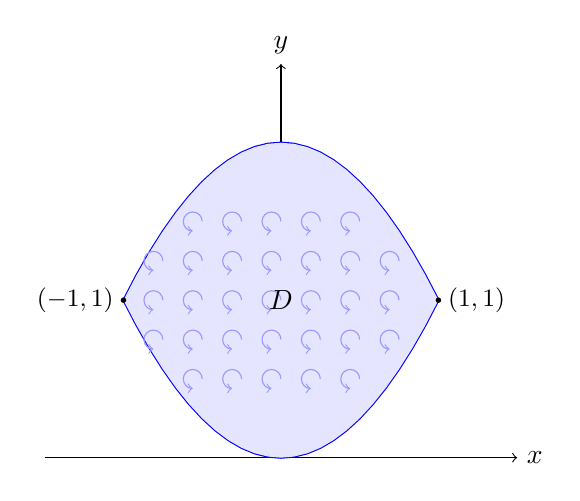
\begin{tikzpicture}[scale=2]
    % Draw axes
    \draw[->] (-1.5,0) -- (1.5,0) node[right] {$x$};
    \draw[->] (0,0) -- (0,2.5) node[above] {$y$};
    
    % Draw parabolas and fill region
    \draw[thick, blue] plot[domain=-1:1] (\x,{2-\x*\x}) node[right] {};
    \draw[thick, blue] plot[domain=-1:1] (\x,{\x*\x}) node[right] {};
    \fill[blue!10] plot[domain=-1:1] (\x,{\x*\x}) -- plot[domain=1:-1] (\x,{2-\x*\x});
    
    % Add vector field visualization with smaller, denser arrows
    \foreach \x in {-0.75,-0.5,-0.25,0,0.25,0.5,0.75} {
        \foreach \y in {0.5,0.75,1,1.25,1.5} {
            \pgfmathparse{(\y < 2-\x*\x-0.1) && (\y > \x*\x+0.1)}
            \ifnum\pgfmathresult=1
                \draw[->, blue!40] (\x,\y) arc (0:270:0.06);
            \fi
        }
    }
    
    
    % Add labels and reference points
    \node at (0,1) {$D$};
    \fill (1,1) circle (0.5pt) node[right] {\small $(1,1)$};
    \fill (-1,1) circle (0.5pt) node[left] {\small $(-1,1)$};
    

\end{tikzpicture}
\caption{\textit{The basin region $D$ bounded by $y=x^2$ and $y=2-x^2$. Blue arrows indicate local vorticity patterns, demonstrating the symmetric flow structure about the vertical axis. This visualization helps us understand why the total vorticity integrates to $8[\sin(1) - \cos(1)]$.}}
\label{fig:flow_basin}
\end{figure}

\begin{solution}
\noindent Rather than tackle this double integral directly, we can exploit the structure of Green's Theorem to transform our area computation into a boundary analysis:

\begin{enumerate}
\item \textbf{Recognition of Pattern}\\
Our vorticity field $f(x,y) = xe^y - y\cos(x)$ mirrors the curl formula $\frac{\partial Q}{\partial x} - \frac{\partial P}{\partial y}$ in Green's Theorem:
\[
\iint_D \left(\frac{\partial Q}{\partial x} - \frac{\partial P}{\partial y}\right)\,dA = \oint_{\partial D} P\,dx + Q\,dy
\]

\item \textbf{Construction of Potential Functions}\\
We identify functions $P$ and $Q$ satisfying our pattern:
\begin{align*}
P(x,y) &= -xe^y \\
Q(x,y) &= -y\sin(x)
\end{align*}

Verification through partial derivatives:
\begin{align*}
\frac{\partial Q}{\partial x} &= -y\cos(x) \\
-\frac{\partial P}{\partial y} &= xe^y
\end{align*}
Therefore: $\frac{\partial Q}{\partial x} - \frac{\partial P}{\partial y} = xe^y - y\cos(x) = f(x,y)$

\item \textbf{Boundary Analysis}\\
Our region's boundary $\partial D$ comprises:
\begin{itemize}
   \item Upper curve: $y = 2-x^2$, traversed from $x = -1$ to $x = 1$
   \item Lower curve: $y = x^2$, traversed from $x = 1$ to $x = -1$
\end{itemize}

\item \textbf{Line Integral Formulation}\\
Along the upper curve ($y = 2-x^2$):
\[
\int_{-1}^1 [-xe^{2-x^2} + 2x(2-x^2)\sin(x)]\,dx
\]

Along the lower curve ($y = x^2$):
\[
\int_{-1}^1 [xe^{x^2} + 2x^3\sin(x)]\,dx
\]

Combining yields:
\[
\int_{-1}^1 [x(e^{x^2} - e^{2-x^2}) + 4x\sin(x)]\,dx
\]

\item \textbf{Symmetry Exploitation}\\
Two key observations simplify our computation:
\begin{itemize}
   \item $x(e^{x^2} - e^{2-x^2})$ is odd on $[-1,1]$, contributing zero to the integral
   \item $4x\sin(x)$ exhibits even symmetry, allowing reduction to $[0,1]$
\end{itemize}

Therefore:
\begin{align*}
\iint_D f(x,y)\,dA &= 8\int_0^1 x\sin(x)\,dx \\
&= 8[\sin(1) - \cos(1)] \\
&\approx 2.4096
\end{align*}
\end{enumerate}

\noindent \textbf{Physical Interpretation:}
The final value of approximately $2.4096$ reveals several key insights about our vorticity field:
\begin{itemize}
   \item The positive result indicates a net counterclockwise rotation in the basin
   \item The moderate magnitude suggests balanced vorticity distribution
   \item The symmetric basin geometry is reflected in our integration technique
   \item Local rotational effects combine to produce measurable global circulation
\end{itemize}

\end{solution}
\end{example}
\exampleline


\subsection*{Big $O$ Notation}

\noindent When we work with limits and approximations in calculus, we often encounter situations where we want to describe how quickly certain terms become negligible as a variable approaches zero. Big $O$ notation provides a precise language for describing these behaviors. \\

\noindent In its simplest form, when we write $f(x) = O(g(x))$ as $x \to a$, we mean that the function $f(x)$ grows no faster than $g(x)$ near $a$. More precisely, there exist constants $M > 0$ and $\delta > 0$ such that:
\[
|f(x)| \leq M|g(x)| \quad \text{whenever } |x-a| < \delta
\]

\noindent For example, in our analysis of Green's Theorem, we encountered terms like:
\[
O(\Delta x^2\Delta y + \Delta x\Delta y^2)
\]
This notation tells us that as $\Delta x$ and $\Delta y$ approach zero, these "error terms" become negligible much faster than the main terms ($\Delta x\Delta y$) in our approximation. \\

\noindent A powerful illustration of this notation appears in the limit definition of the derivative. Consider finding $\frac{d}{dx}(x^n)$ using first principles:
\begin{align*}
\frac{d}{dx}(x^n) &= \lim_{h \to 0} \frac{(x+h)^n - x^n}{h} \\
&= \lim_{h \to 0} \frac{x^n + nx^{n-1}h + \frac{n(n-1)}{2}x^{n-2}h^2 + O(h^3) - x^n}{h} \\
&= \lim_{h \to 0} \left(nx^{n-1} + \frac{n(n-1)}{2}x^{n-2}h + O(h^2)\right) \\
&= nx^{n-1}
\end{align*}

\noindent Here, $O(h^3)$ captures all terms with powers of $h$ greater than 2 in the binomial expansion, and after dividing by $h$, these terms become $O(h^2)$. As $h \to 0$, these higher-order terms vanish, leaving us with our familiar result. \\

\noindent Think of Big $O$ notation as a way of classifying the "speed" at which functions approach zero:
\begin{itemize}
   \item $O(\Delta x)$ approaches zero linearly
   \item $O(\Delta x^2)$ approaches zero quadratically (much faster)
   \item $O(\Delta x^3)$ approaches zero even faster
\end{itemize}

\noindent In our proof of Green's Theorem, when we write:
\[
Q(x+\Delta x,y) = Q(x,y) + \frac{\partial Q}{\partial x}\Delta x + O(\Delta x^2)
\]
we're saying that the error in our linear approximation shrinks quadratically as $\Delta x \to 0$. This precision in describing approximation errors is crucial for establishing the validity of our limiting arguments.

\begin{figure}[H]
\centering
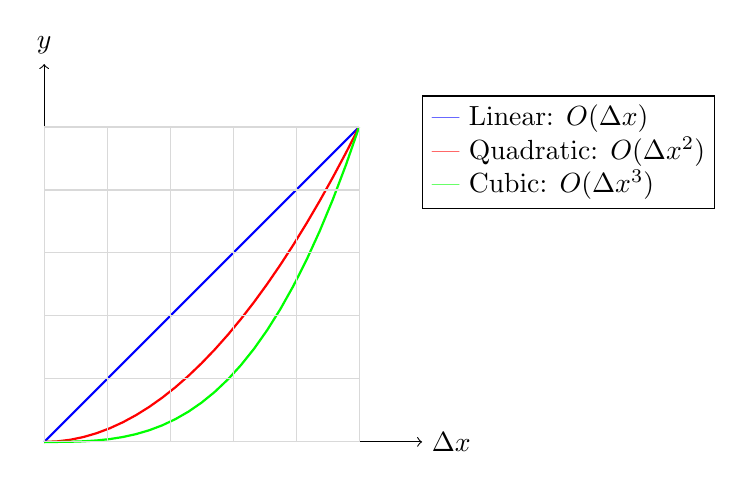
\begin{tikzpicture}[scale=4]
   % Draw axes
   \draw[->] (0,0) -- (1.2,0) node[right] {$\Delta x$};
   \draw[->] (0,0) -- (0,1.2) node[above] {$y$};
   
   % Plot functions
   \draw[blue, thick, domain=0:1] plot (\x, \x);
   \draw[red, thick, domain=0:1] plot (\x, {\x*\x});
   \draw[green, thick, domain=0:1] plot (\x, {\x*\x*\x});
   
   % Add grid
   \draw[gray!30] (0,0) grid[step=0.2] (1,1);
   
   % Add legend
   \node[anchor=north west, draw, fill=white, align=left] at (1.2,1.1) {
       \textcolor{blue}{---} Linear: $O(\Delta x)$\\
       \textcolor{red}{---} Quadratic: $O(\Delta x^2)$\\
       \textcolor{green}{---} Cubic: $O(\Delta x^3)$
   };
\end{tikzpicture}
\caption{\textit{Comparison of convergence rates as $\Delta x \to 0$. Each curve represents a different order of convergence, demonstrating how higher-order terms approach zero more rapidly. This visualization helps us understand why we can neglect higher-order terms in limit computations.}}
\label{fig:big_o}
\end{figure}

\noindent This notation proves invaluable in calculus as it allows us to focus on dominant terms in approximations and streamline complex limit computations by isolating key terms.



\newpage

\lecture{Curl and Divergence} \index{Curl}\index{Divergence}

\noindent Vector fields appear throughout mathematics and physics—they might represent fluid flow, gravitational forces, or electric fields. While we can visualize these fields through arrows showing direction and magnitude at each point, we often need more sophisticated tools to analyze their behavior. Two fundamental concepts help us understand how vector fields behave locally: curl, which measures rotation, and divergence, which measures expansion or contraction. These operators provide powerful tools for analyzing fluid flow, electromagnetic fields, and many other physical phenomena. \\

\noindent Way back in Chapter 1, we encountered the cross product of vectors—an operation that produced a vector perpendicular to two given vectors, with magnitude related to the parallelogram they formed. This geometric interpretation of the cross product will now take on new life as we use it to measure rotation in vector fields. Similarly, the dot product, which measured how much vectors pointed in the same direction, will help us quantify how much vector fields expand or contract. \\

\noindent The beauty of these concepts lies in how they bridge local and global behaviors. Just as derivatives in single-variable calculus measure instantaneous rates of change, curl and divergence measure instantaneous rotation and expansion in vector fields. And just as integration gives us global information about functions, theorems involving curl and divergence connect local and global properties of vector fields. We will also see an important generalization of Green's Theorem which we touched upon briefly after our proof.

\subsection*{Curl: Measuring Rotation}

\noindent Imagine stirring a cup of coffee. As your spoon moves through the liquid, it creates a swirling motion—the coffee rotates around points in the fluid. This everyday observation leads us to a profound question in vector calculus: How can we mathematically measure the ``amount of rotation" at any point in a vector field? \\

\noindent In the previous lecture, we approached rotation from a global perspective through Green's Theorem, relating the total rotation within a region to the behavior of the field along its boundary. Now we'll zoom in and examine rotation at individual points, stripping away the accumulation of rotational effects to understand the fundamental local behavior. Just as derivatives in single-variable calculus helped us understand rates of change at a point, we'll develop tools to understand rotation at a point. This local perspective will prove invaluable especially from fluid dynamics to electromagnetic theory, for which we will take a few examples. \\

\noindent To approach this systematically, let's start with perhaps the simplest rotating system: a rigid disk spinning with angular velocity $\omega$. From basic physics, we know that a point at radius $r$ from the center moves with speed $v = \omega r$. This linear relationship between speed and radius creates a vector field of velocities:

\begin{figure}[H]
\centering
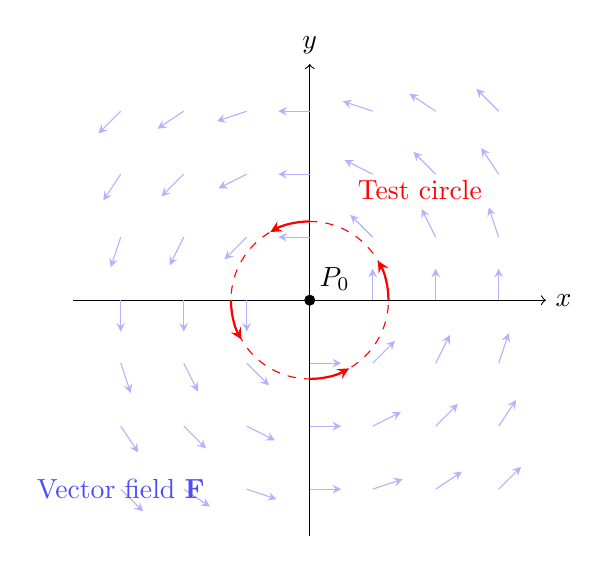
\begin{tikzpicture}[scale=2]
    % Draw axes
    \draw[->] (-1.5,0) -- (1.5,0) node[right] {$x$};
    \draw[->] (0,-1.5) -- (0,1.5) node[above] {$y$};
    
    % Draw the background vector field (normalized, lighter)
    \foreach \x in {-1.2,-0.8,...,1.2} {
        \foreach \y in {-1.2,-0.8,...,1.2} {
            \pgfmathsetmacro{\len}{sqrt(\x*\x+\y*\y)}
            \pgfmathparse{\len > 0.1 ? 1 : 0}
            \if\pgfmathresult1
                \draw[-stealth, blue!30, thin] (\x,\y) -- 
                    +({-0.2*\y/\len},{0.2*\x/\len});
            \fi
        }
    }
    
    % Draw a test circle (dashed, with orientation)
    \draw[red, dashed] (0,0) circle (0.5);
    \foreach \angle in {0,90,180,270} {
        \draw[-stealth, red, thick] 
            ({0.5*cos(\angle)},{0.5*sin(\angle)}) 
            arc (\angle:\angle+30:0.5);
    }
    
    % Label center point P
    \fill (0,0) circle (1pt) node[above right] {$P_0$};
    
    % Add explanatory labels
    \node[red] at (0.7,0.7) {Test circle};
    \node[blue!70] at (-1.2,-1.2) {Vector field $\mathbf{F}$};
\end{tikzpicture}
\caption{\textit{To measure rotation at point $P_0$, we probe the vector field $\mathbf{F}$ using a counterclockwise-oriented test circle (red, dashed). The background shows the normalized vector field. At each point on our test circle, we'll compare how well the vector field aligns with the circle's orientation.}}
\label{fig:curl_probe}
\end{figure}

\noindent Given any vector field $\mathbf{F}$ and any point $P_0$ in its domain, we can investigate rotation by examining how $\mathbf{F}$ interacts with a geometric probe - specifically, a counterclockwise-oriented `test' circle we draw centered at $P_0$. When we examine the vector field values $\mathbf{F}$ at points along this circle, we notice that some vectors align more closely with our circle's orientation than others. This alignment pattern (or lack thereof) reveals the rotational tendency of $\mathbf{F}$ at $P_0$. We can capture this behavior precisely through a line integral, measuring how much $\mathbf{F}$ ``follows along" our test circle $C_r$ of radius $r$:
\[
\oint_{C_r} \mathbf{F} \cdot d\mathbf{r}
\]
Here, the dot product naturally compares the field's alignment with our circular path at each point, while the integral sums these contributions around the entire circle. But here's the clever part: if we want to measure the ``rotation per unit area," we should divide by the circle's area (similar to how we calculated our average efficiency problem from Chapter 4):
\[
\frac{1}{\pi r^2} \oint_{C_r} \mathbf{F} \cdot d\mathbf{r}
\]

\noindent Now, what happens as we make our circle smaller and smaller? We get closer to measuring the pure rotational tendency at point $P$:
\[
\lim_{r \to 0} \frac{1}{\pi r^2} \oint_{C_r} \mathbf{F} \cdot d\mathbf{r}
\]

\begin{figure}[H]
\centering
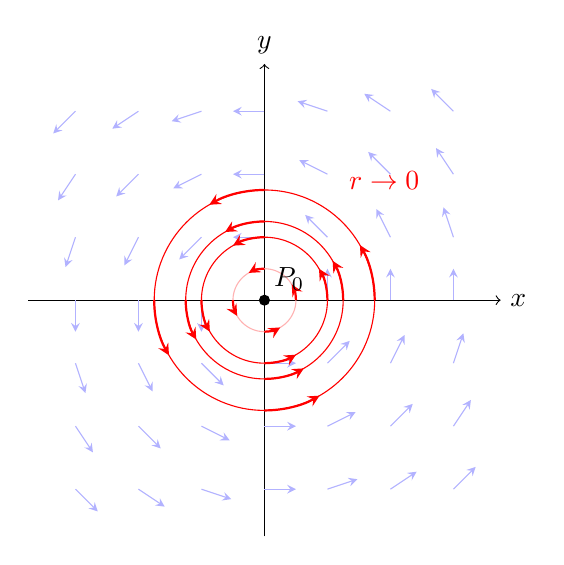
\begin{tikzpicture}[scale=2]
    % Draw axes
    \draw[->] (-1.5,0) -- (1.5,0) node[right] {$x$};
    \draw[->] (0,-1.5) -- (0,1.5) node[above] {$y$};
    
    % Draw the background vector field (normalized, lighter)
    \foreach \x in {-1.2,-0.8,...,1.2} {
        \foreach \y in {-1.2,-0.8,...,1.2} {
            \pgfmathsetmacro{\len}{sqrt(\x*\x+\y*\y)}
            \pgfmathparse{\len > 0.1 ? 1 : 0}
            \if\pgfmathresult1
                \draw[-stealth, blue!30, thin] (\x,\y) -- 
                    +({-0.2*\y/\len},{0.2*\x/\len});
            \fi
        }
    }

    % Draw a test circle (dashed, with orientation)
    \draw[red] (0,0) circle (0.7);
    \foreach \angle in {0,90,180,270} {
        \draw[-stealth, red, thick] 
            ({0.7*cos(\angle)},{0.7*sin(\angle)}) 
            arc (\angle:\angle+30:0.7);
    }
    
    % Draw a test circle (dashed, with orientation)
    \draw[red] (0,0) circle (0.5);
    \foreach \angle in {0,90,180,270} {
        \draw[-stealth, red, thick] 
            ({0.5*cos(\angle)},{0.5*sin(\angle)}) 
            arc (\angle:\angle+30:0.5);
    }

    % Draw a test circle (dashed, with orientation)
    \draw[red] (0,0) circle (0.4);
    \foreach \angle in {0,90,180,270} {
        \draw[-stealth, red, thick] 
            ({0.4*cos(\angle)},{0.4*sin(\angle)}) 
            arc (\angle:\angle+30:0.4);
    }

    % Draw a test circle (dashed, with orientation)
    \draw[red!30] (0,0) circle (0.2);
    \foreach \angle in {0,90,180,270} {
        \draw[-stealth, red, thick] 
            ({0.2*cos(\angle)},{0.2*sin(\angle)}) 
            arc (\angle:\angle+30:0.2);
    }
    
    % Label center point P
    \fill (0,0) circle (1pt) node[above right] {$P_0$};
    
    % Add explanatory labels
    \node[red] at (0.76,0.76) {$r \to 0$};
\end{tikzpicture}
\caption{\textit{As we shrink the circular path around point $P_0$, we measure the local rotational tendency of the field.}}
\label{fig:shrinking_circles}
\end{figure}

\noindent Through careful mathematical analysis, this limit equals:
\[
\frac{\partial Q}{\partial x} - \frac{\partial P}{\partial y}.
\]

\noindent To see this *deep breath*, parameterize the circle $C_r$ of radius $r$ centered at $P_0 = (x_0, y_0)$ using $x = x_0 + r \cos\theta$ and $y = y_0 + r \sin\theta$, where $\theta \in [0, 2\pi]$. The line integral for $\mathbf{F} = P\mathbf{i} + Q\mathbf{j}$ becomes:
\[
\oint_{C_r} \mathbf{F} \cdot d\mathbf{r} = \int_0^{2\pi} \big(P(x_0 + r \cos\theta, y_0 + r \sin\theta)(-r \sin\theta) + Q(x_0 + r \cos\theta, y_0 + r \sin\theta)(r \cos\theta)\big) d\theta.
\]

\noindent Expanding $P$ and $Q$ about $(x_0, y_0)$ using a first-order Taylor approximation:
\[
P(x_0 + r \cos\theta, y_0 + r \sin\theta) \approx P(x_0, y_0) + \frac{\partial P}{\partial x} r \cos\theta + \frac{\partial P}{\partial y} r \sin\theta,
\]
\[
Q(x_0 + r \cos\theta, y_0 + r \sin\theta) \approx Q(x_0, y_0) + \frac{\partial Q}{\partial x} r \cos\theta + \frac{\partial Q}{\partial y} r \sin\theta.
\]

\noindent Substitute these approximations into the integral. Expanding and collecting terms, we observe that the contributions from $P(x_0, y_0)$ and $Q(x_0, y_0)$ involve factors of $\sin\theta$ and $\cos\theta$, respectively:
\[
\int_0^{2\pi} P(x_0, y_0)(-r \sin\theta) \, d\theta = 0, \quad \int_0^{2\pi} Q(x_0, y_0)(r \cos\theta) \, d\theta = 0,
\]
because the integrals of $\sin\theta$ and $\cos\theta$ over $[0, 2\pi]$ are zero. \\

\noindent Next, consider the first-order terms involving $\frac{\partial P}{\partial x}$, $\frac{\partial P}{\partial y}$, $\frac{\partial Q}{\partial x}$, and $\frac{\partial Q}{\partial y}$:
\[
\int_0^{2\pi} \left(-\frac{\partial P}{\partial x} r^2 \cos\theta \sin\theta - \frac{\partial P}{\partial y} r^2 \sin^2\theta + \frac{\partial Q}{\partial x} r^2 \cos^2\theta + \frac{\partial Q}{\partial y} r^2 \cos\theta \sin\theta\right) d\theta.
\]

\noindent The terms proportional to $\cos\theta \sin\theta$ also vanish because:
\[
\int_0^{2\pi} \cos\theta \sin\theta \, d\theta = 0.
\]
\noindent The remaining terms simplify using:
\[
\int_0^{2\pi} \cos^2\theta \, d\theta = \int_0^{2\pi} \sin^2\theta \, d\theta = \pi.
\]

\noindent Thus, the integral reduces to:
\[
\oint_{C_r} \mathbf{F} \cdot d\mathbf{r} = r^2 \pi \left(\frac{\partial Q}{\partial x} - \frac{\partial P}{\partial y}\right).
\]


\noindent Dividing by $\pi r^2$ and taking the limit as $r \to 0$, we obtain:
\[
\frac{\partial Q}{\partial x} - \frac{\partial P}{\partial y}.
\]

\noindent This result can be generalized to three dimensions. In 2D the single number $Q_x - P_y$ was enough to describe rotation because there is only one plane to rotate in. But in 3D, rotation at a point has \textit{two} pieces of information: \textbf{which axis} the field is spinning around, and \textbf{how fast}. The natural way to encode both is a single vector. That vector is the \textit{curl} of $\mathbf{F}$: its \textbf{direction} is the axis of fastest spinning (determined by the right-hand rule), and its \textbf{magnitude} is the rate of that rotation. The three components of the curl measure the rotation in each of the three coordinate planes ($yz$, $xz$, $xy$), which is exactly how many independent planes exist in $\mathbb{R}^3$. \\ \\
\noindent For a vector field $\mathbf{F}(x,y,z) = P\,\mathbf{i} + Q\,\mathbf{j} + R\,\mathbf{k}$, the curl is computed via the symbolic determinant:
\[
\nabla \times \mathbf{F} =
\begin{vmatrix}
\mathbf{i} & \mathbf{j} & \mathbf{k} \\
\frac{\partial}{\partial x} & \frac{\partial}{\partial y} & \frac{\partial}{\partial z} \\
P & Q & R
\end{vmatrix}
= \left( \frac{\partial R}{\partial y} - \frac{\partial Q}{\partial z} \right)\mathbf{i}
+ \left( \frac{\partial P}{\partial z} - \frac{\partial R}{\partial x} \right)\mathbf{j}
+ \left( \frac{\partial Q}{\partial x} - \frac{\partial P}{\partial y} \right)\mathbf{k}.
\]
For two-dimensional vector fields, where the field is given by 
\(\mathbf{F}(x,y) = P(x,y)\,\mathbf{i} + Q(x,y)\,\mathbf{j}\) (i.e. with \(R(x,y)=0\)),
the curl reduces to a vector having only a \(z\)-component:
\[
\nabla \times \mathbf{F} = \left( 0,\,0,\,\frac{\partial Q}{\partial x} - \frac{\partial P}{\partial y} \right).
\]
It is common in the plane to refer to the scalar 
\[
\frac{\partial Q}{\partial x} - \frac{\partial P}{\partial y}
\]
as the curl, with a positive value indicating counterclockwise rotation and a negative value indicating clockwise rotation.

\subsubsection*{Beyond Three Dimensions: Why Curl is a Vector Only in $\mathbb{R}^3$}

\noindent Each component of the curl measures rotation in a particular coordinate plane. In $\mathbb{R}^3$ there are $\binom{3}{2} = 3$ coordinate planes ($xy$, $xz$, $yz$), and the dimension is also $3$. This numerical coincidence lets us package the three rotation measurements as a vector. In any other dimension, the number of planes differs from the dimension, and the ``curl'' can no longer be a vector:

\begin{center}
\begin{tabular}{c|c|c|l}
\toprule
$n$ & Planes $\binom{n}{2}$ & \textbf{Curl is a\ldots} & \textbf{Notes} \\
\midrule
2 & 1 & scalar & The $Q_x - P_y$ from Green's Theorem \\
3 & 3 & vector & The familiar $\nabla \times \mathbf{F}$ \\
4 & 6 & $4\times 4$ antisymmetric matrix & Called a \textit{2-form} in differential geometry \\
$n$ & $\frac{n(n-1)}{2}$ & $n\times n$ antisymmetric matrix & Entries $C_{ij} = \partial_i F_j - \partial_j F_i$ \\
\bottomrule
\end{tabular}
\end{center}

\noindent Only when $n = 3$ does $\binom{n}{2} = n$. This is why the curl---and the cross product $\mathbf{a} \times \mathbf{b}$---are specific to three dimensions. \\

\noindent \textbf{A payoff from physics.} In Einstein's special relativity, spacetime is four-dimensional. The electromagnetic potential $A_\mu = (\phi, A_x, A_y, A_z)$ has a 4D ``curl''---the antisymmetric matrix $F_{\mu\nu} = \partial_\mu A_\nu - \partial_\nu A_\mu$---called the \textbf{electromagnetic field tensor}:
\[
F_{\mu\nu} = \begin{pmatrix}
0 & E_x & E_y & E_z \\
-E_x & 0 & -B_z & B_y \\
-E_y & B_z & 0 & -B_x \\
-E_z & -B_y & B_x & 0
\end{pmatrix}
\]
Its six independent entries are the three components of the electric field $\mathbf{E}$ and the three components of the magnetic field $\mathbf{B}$. Electricity and magnetism are not two separate phenomena---they are the six components of a single 4D curl.

\bigskip

\noindent \textbf{Reading curl one component at a time.} Each component of $\nabla\times\mathbf{F}$ measures rotation in the coordinate plane perpendicular to that component's axis. To find the rotation in a particular plane, just ``look down'' that axis at the 2D cross-section:

\begin{itemize}
    \item \textbf{$\mathbf{k}$-component} ($Q_x - P_y$): measures rotation in the $xy$-plane. This is what we see when we look down the $z$-axis---exactly the 2D curl from Green's Theorem.
    \item \textbf{$\mathbf{i}$-component} ($R_y - Q_z$): measures rotation in the $yz$-plane. Look down the $x$-axis, and ask whether the field swirls in the $yz$-plane.
    \item \textbf{$\mathbf{j}$-component} ($P_z - R_x$): measures rotation in the $xz$-plane. Look down the $y$-axis.
\end{itemize}

\noindent The pattern follows from the cyclic structure of the cross product: $\mathbf{j}\times\mathbf{k} = \mathbf{i}$ tells us the $yz$-plane rotation points along $\mathbf{i}$; $\mathbf{k}\times\mathbf{i} = \mathbf{j}$ tells us $xz$-rotation points along $\mathbf{j}$; and $\mathbf{i}\times\mathbf{j} = \mathbf{k}$ tells us $xy$-rotation points along $\mathbf{k}$. In 3D, the full curl vector is the sum of these three independent rotations, one per coordinate plane. The figures below illustrate this for the $xy$-plane (looking down the $z$-axis), so only the $\mathbf{k}$-component is visible.

%https://tikz.net/curl/     Izaak Neutelings
\begin{figure}[H]
\centering
\colorlet{veccol}{orange!90!black}
\colorlet{myblue}{blue!60!black}
\tikzstyle{vector}=[->,thick,veccol]
\def\R{1.4}
\def\r{0.03}
\def\ang{60}
\def\N{6}

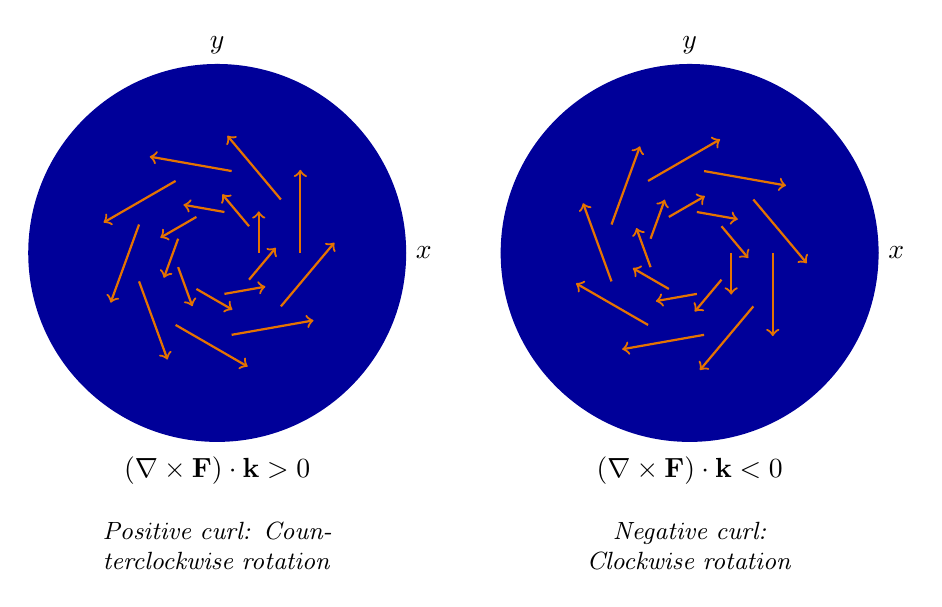
\begin{tikzpicture}[scale=1.2]
    % First diagram: Positive curl (counterclockwise)
    \begin{scope}[xshift=-2.5cm]
        % Axes
        \draw[thin, ->] (-2,0) -- (2,0) node[right] {$x$};
        \draw[thin, ->] (0,-2) -- (0,2) node[above] {$y$};
        
        % Central point
        \fill[myblue] (0,0) circle (\r);
        
        % Rotational vectors (counterclockwise)
        \foreach \R in {0.44,0.88}{
            \foreach \i [evaluate={\ang=\i*360/\N;}] in {1,...,\N}{
                \draw[vector] (\ang:\R) --++ (\ang+90:\R);
            }
        }
        
        % Label with mathematical notation
        \node at (0,-2.3) {$(\nabla \times \mathbf{F})\cdot\mathbf{k} > 0$};
        \node[text width=3cm, align=center, font=\small] at (0,-3.1)
            {\textit{Positive curl: Counterclockwise rotation}};
    \end{scope}
    
    % Second diagram: Negative curl (clockwise)
    \begin{scope}[xshift=2.5cm]
        % Axes
        \draw[thin, ->] (-2,0) -- (2,0) node[right] {$x$};
        \draw[thin, ->] (0,-2) -- (0,2) node[above] {$y$};
        
        % Central point
        \fill[myblue] (0,0) circle (\r);
        
        % Rotational vectors (clockwise)
        \foreach \R in {0.44,0.88}{
            \foreach \i [evaluate={\ang=\i*360/\N;}] in {1,...,\N}{
                \draw[vector] (\ang:\R) --++ (\ang-90:\R);
            }
        }
        
        % Label with mathematical notation
        \node at (0,-2.3) {$(\nabla \times \mathbf{F})\cdot\mathbf{k} < 0$};
        \node[text width=3cm, align=center, font=\small] at (0,-3.1)
            {\textit{Negative curl: Clockwise rotation}};
    \end{scope}
    
\end{tikzpicture}
\caption{\textit{Patterns of curl in 2D vector fields. Left: the $\mathbf{k}$-component of $\nabla\times\mathbf{F}$ is positive, corresponding to counterclockwise rotation. Right: negative, corresponding to clockwise. Since curl is a \textbf{vector}, the sign refers to its $\mathbf{k}$-component (the only nonzero component for a 2D field).}}
\label{fig:curl_patterns}
\end{figure}

\noindent We have several situations that arise where there is no rotation (also called irrotation). Below we depict them:

%https://tikz.net/curl/     Izaak Neutelings
\begin{figure}[H]
\centering
\colorlet{veccol}{orange!90!black}
\colorlet{myblue}{blue!60!black}
\tikzstyle{vector}=[->,thick,veccol]
\def\R{1.4}
\def\r{0.03}
\def\N{9}
\def\null{\color{myblue}{0}}

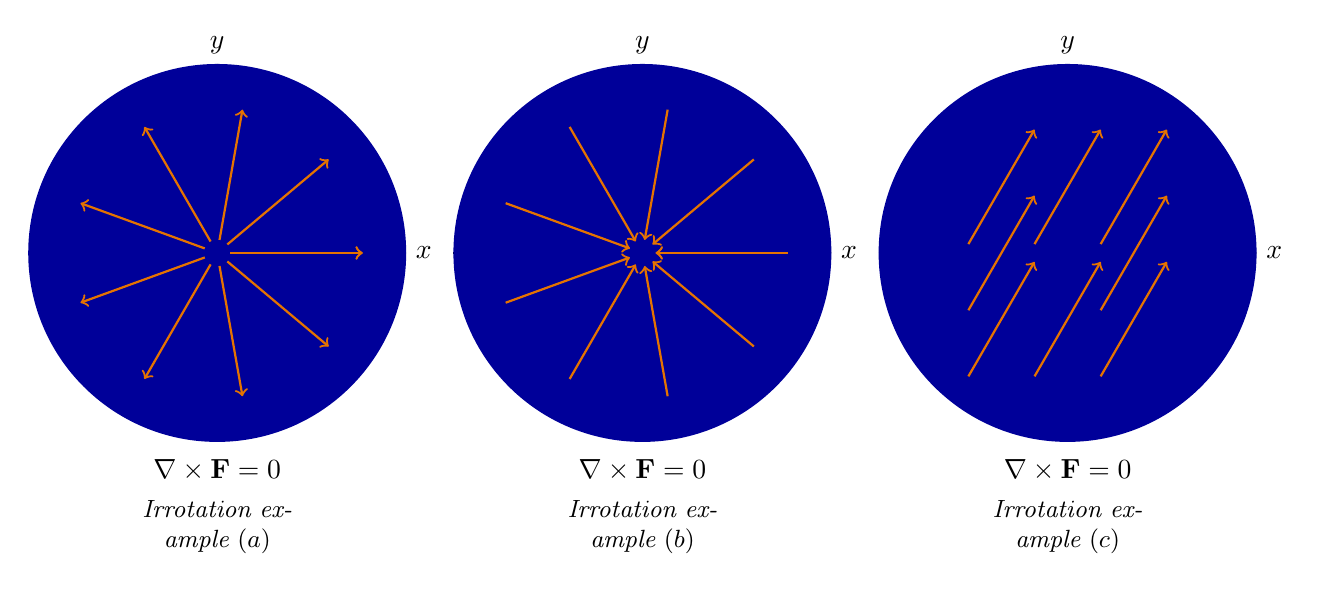
\begin{tikzpicture}[scale=1.2]
    % First diagram: Source field
    \begin{scope}[xshift=-4.5cm]
        % Axes
        \draw[thin, ->] (-2,0) -- (2,0) node[right] {$x$};
        \draw[thin, ->] (0,-2) -- (0,2) node[above] {$y$};
        
        % Central point
        \fill[myblue] (0,0) circle (\r);
        
        % Radial vectors with consistent spacing
        \foreach \i [evaluate={\ang=\i*360/\N;}] in {0,...,\N}{
            \draw[vector] (\ang:0.1*\R) --++ (\ang:\R);
        }
        
        % Label with mathematical notation
        \node at (0,-2.3) {$\nabla \times \mathbf{F} = 0$};
        \node[text width=3cm, align=center, font=\small] at (0,-2.9) 
            {\textit{Irrotation example $(a)$}};
    \end{scope}
    
    % Second diagram: Sink field
    \begin{scope}[xshift=0cm]
        % Axes
        \draw[thin, ->] (-2,0) -- (2,0) node[right] {$x$};
        \draw[thin, ->] (0,-2) -- (0,2) node[above] {$y$};
        
        % Central point
        \fill[myblue] (0,0) circle (\r);
        
        % Radial vectors pointing inward
        \foreach \i [evaluate={\ang=\i*360/\N;}] in {0,...,\N}{
            \draw[vector] (\ang:1.1*\R) -- (\ang:0.1*\R);
        }
        
        % Label with mathematical notation
        \node at (0,-2.3) {$\nabla \times \mathbf{F} = 0$};
        \node[text width=3cm, align=center, font=\small] at (0,-2.9) 
            {\textit{Irrotation example $(b)$}};
    \end{scope}
    
    % Third diagram: Incompressible flow
    \begin{scope}[xshift=4.5cm]
        % Axes
        \draw[thin, ->] (-2,0) -- (2,0) node[right] {$x$};
        \draw[thin, ->] (0,-2) -- (0,2) node[above] {$y$};
        
        % Central point
        \fill[myblue] (0,0) circle (\r);
        
        % Parallel flow pattern
        \def\ang{60}
        \foreach \x/\y in {-1/0,-1/1,0/1,1/1,1/0,-1/-1,0/-1,1/-1}{
            \draw[vector] (\x*0.5*\R,\y*0.5*\R) ++ (\ang-180:\R/2) --++ (\ang:\R);
        }
        
        % Label with mathematical notation
        \node at (0,-2.3) {$\nabla \times \mathbf{F} = 0$};
        \node[text width=3cm, align=center, font=\small] at (0,-2.9) 
            {\textit{Irrotation example $(c)$}};
    \end{scope}
\end{tikzpicture}
\caption{\textit{Three very different vector field patterns, all with zero curl. The arrows clearly show no local rotation about the center point: a tiny paddlewheel placed there would not spin. (a) Source / radial outflow. (b) Sink / radial inflow. (c) Uniform parallel flow.}}
\label{fig:zero_curl_patterns}
\end{figure}

\subsubsection*{The Paddlewheel Test: Understanding Positive and Negative Curl}

\noindent The figures above illustrate the extremes: pure counterclockwise rotation, pure clockwise rotation, and no rotation at all. But the real power of curl lies in detecting rotation in fields that don't \textit{look} like they're spinning. Consider the \textbf{shear flow}:
\[
\mathbf{F}(x,y) = y\,\mathbf{i}
\]

\noindent Every vector points horizontally. Vectors above the $x$-axis point right; vectors below point left. There are no circular streamlines, no obvious ``swirling." Yet the 2D curl is:
\[
\frac{\partial Q}{\partial x} - \frac{\partial P}{\partial y} = 0 - 1 = -1
\]

\noindent The curl is \textit{negative}. How can a field with purely horizontal, straight arrows have rotation?

\medskip

\noindent The answer lies in the \textbf{paddlewheel test}. Imagine placing a tiny paddlewheel (like a pinwheel) at a point in the flow. The fluid pushes on each blade of the wheel. If the flow is faster or differently directed on one side of the wheel than the other, the asymmetric forces create a torque, and the wheel spins.

\begin{figure}[H]
\centering
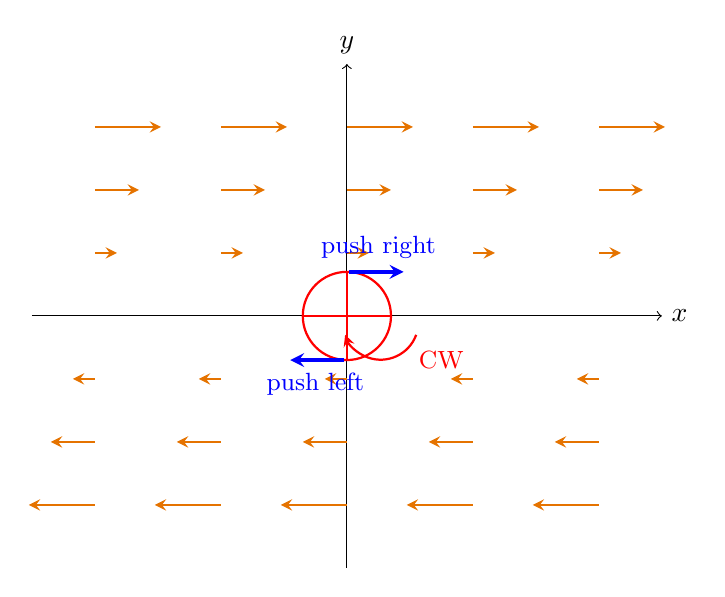
\begin{tikzpicture}[scale=1.6]
    % Draw axes
    \draw[->] (-2.5,0) -- (2.5,0) node[right] {$x$};
    \draw[->] (0,-2) -- (0,2) node[above] {$y$};

    % Draw the shear field F = <y, 0>
    \foreach \x in {-2,-1,0,1,2} {
        \foreach \y in {-1.5,-1,-0.5,0.5,1,1.5} {
            \draw[-stealth, orange!90!black, thick] (\x,\y) -- +(\y*0.35, 0);
        }
    }

    % Draw paddlewheel at origin
    \draw[thick, red] (0,0) circle (0.35);
    \draw[thick, red] (-0.35,0) -- (0.35,0);
    \draw[thick, red] (0,-0.35) -- (0,0.35);

    % Annotation arrows showing force on top vs bottom of wheel
    \draw[-stealth, blue, very thick] (0.02,0.35) -- (0.45,0.35);
    \node[blue, font=\small, above] at (0.25,0.38) {push right};
    \draw[-stealth, blue, very thick] (-0.02,-0.35) -- (-0.45,-0.35);
    \node[blue, font=\small, below] at (-0.25,-0.38) {push left};

    % Rotation arrow
    \draw[-stealth, red, thick] (0.55,-0.15) arc (-20:-160:0.3);
    \node[red, font=\small] at (0.75,-0.35) {CW};
\end{tikzpicture}
\caption{\textit{The paddlewheel test for shear flow $\mathbf{F} = \langle y, 0 \rangle$. Vectors above the $x$-axis push the top blade to the right; vectors below push the bottom blade to the left. The imbalance creates clockwise rotation, confirming the negative curl.}}
\label{fig:paddlewheel_shear}
\end{figure}

\noindent In the shear flow above:
\begin{itemize}
    \item The \textit{top} of the paddlewheel sits at $y > 0$, where the flow pushes rightward.
    \item The \textit{bottom} sits at $y < 0$, where the flow pushes leftward.
    \item Together, these asymmetric forces spin the wheel \textbf{clockwise}.
\end{itemize}

\noindent Clockwise rotation corresponds to \textbf{negative curl}. Counterclockwise rotation corresponds to \textbf{positive curl}. The magnitude of the curl measures how fast the wheel spins. More precisely:

\begin{itemize}
    \item \textbf{Positive curl} ($\nabla \times \mathbf{F}$ in the $+\mathbf{k}$ direction): the paddlewheel spins counterclockwise (CCW). By the right-hand rule, curling your fingers CCW makes your thumb point out of the page.
    \item \textbf{Negative curl} ($\nabla \times \mathbf{F}$ in the $-\mathbf{k}$ direction): the paddlewheel spins clockwise (CW). Curling your fingers CW makes your thumb point into the page.
    \item \textbf{Zero curl}: the paddlewheel does not spin, regardless of how fast the fluid is moving.
\end{itemize}

\noindent In three dimensions, $\nabla \times \mathbf{F}$ is a full vector: its \textit{direction} is the axis about which the paddlewheel spins fastest (determined by the right-hand rule), and its \textit{magnitude} is the rate of that rotation.

\medskip

\noindent \textbf{A crucial subtlety.} Curl measures \textit{local} rotation at a point, not the global shape of the flow's streamlines. Consider two instructive cases:
\begin{enumerate}
    \item A field can have \textbf{straight streamlines but nonzero curl}: the shear flow $\mathbf{F} = \langle y, 0 \rangle$ has perfectly straight, horizontal streamlines, yet curl $= -1$ everywhere. The velocity gradient across the flow creates a torque on the paddlewheel.
    \item A field can have \textbf{curved streamlines but zero curl}: the vortex field $\mathbf{F} = \frac{\langle -y, x \rangle}{x^2 + y^2}$ (away from the origin) has circular streamlines, yet curl $= 0$. The velocity decreases with distance from the origin in just the right way to prevent any net torque on a paddlewheel---the outer streamlines are slower than the inner ones by exactly the right amount to balance out the curvature.
\end{enumerate}

\noindent What matters is not whether the streamlines \textit{look} circular, but whether nearby parts of the flow create a torque---an imbalance of forces---on a tiny paddlewheel.

\exampleline
\begin{example}
Determine the 2D curl of each velocity field and describe the paddlewheel behavior at the origin.

\begin{enumerate}
    \item $\mathbf{F} = \langle 0, x \rangle$ \quad (vertical shear)
    \item $\mathbf{F} = \langle -y, 0 \rangle$ \quad (horizontal shear, reversed)
    \item $\mathbf{F} = \langle y, x \rangle$
\end{enumerate}

\begin{solution}
\begin{enumerate}
    \item $\text{curl}\,\mathbf{F} = Q_x - P_y = 1 - 0 = 1$ (\textbf{positive}, CCW).

    \textit{Paddlewheel picture:} At the origin, the right blade ($x > 0$) feels an upward push, while the left blade ($x < 0$) feels a downward push. This creates counterclockwise rotation. All arrows are purely vertical, yet the field has curl---through \textit{vertical} shear rather than horizontal shear.

    \item $\text{curl}\,\mathbf{F} = Q_x - P_y = 0 - (-1) = 1$ (\textbf{positive}, CCW).

    \textit{Paddlewheel picture:} The top blade ($y > 0$) is pushed leftward, and the bottom blade ($y < 0$) is pushed rightward. This is again counterclockwise. Despite looking very different from (a), both fields have the same curl!

    \item $\text{curl}\,\mathbf{F} = Q_x - P_y = 1 - 1 = 0$ (\textbf{irrotational}).

    \textit{Paddlewheel picture:} The $P = y$ component pushes the top blade right and the bottom left (CW tendency). But the $Q = x$ component pushes the right blade up and the left blade down (CCW tendency). These two effects exactly cancel, so the paddlewheel doesn't spin. In fact, $\mathbf{F} = \nabla(xy)$, confirming the field is conservative.
\end{enumerate}
\end{solution}
\end{example}
\exampleline

\subsubsection*{Green's Theorem Reformulated}
\noindent Green's Theorem is intimately related to the curl of a vector field. In two dimensions, for a vector field 
\(\mathbf{F}(x,y) = P(x,y)\,\mathbf{i} + Q(x,y)\,\mathbf{j}\),
we recognize that the full three-dimensional curl reduces to:
\[
\nabla \times \mathbf{F} = \left(0,\,0,\,\frac{\partial Q}{\partial x} - \frac{\partial P}{\partial y}\right).
\]
Thus, we often denote the scalar 
\(\frac{\partial Q}{\partial x} - \frac{\partial P}{\partial y}\) 
as the curl, which measures the rotational tendency (about the \(z\)-axis) of the field at each point. Substituting this scalar curl into Green's Theorem, we obtain:
\[
\oint_{\partial D} \mathbf{F} \cdot d\mathbf{r} = \iint_D \left(\frac{\partial Q}{\partial x} - \frac{\partial P}{\partial y}\right) dA.
\]
This formulation connects the circulation around the boundary \(\partial D\) to the net rotation within the region \(D\).

\exampleline
\begin{example}
The electric field in a region of space exhibits complex oscillatory behavior. Consider a simplified model of such a field given by:
\[
\mathbf{F}(x,y,z) = e^{x} \cos(y)\mathbf{i} + e^{y} \sin(z)\mathbf{j} + e^{z} \cos(x)\mathbf{k}
\]
Calculate $\text{curl }\mathbf{F}$ and interpret its physical meaning.

\begin{solution}
Let's compute the curl of the vector field $\mathbf{F}(x,y,z)$ systematically.

\begin{enumerate}
\item \textbf{Identify the Components:}
\[
P = e^{x} \cos(y), \quad Q = e^{y} \sin(z), \quad R = e^{z} \cos(x)
\]

\item \textbf{Recall the Formula for Curl:}
In three dimensions, the curl of $\mathbf{F}$ is given by:
\[
\text{curl }\mathbf{F} = \nabla \times \mathbf{F} = \left(\frac{\partial R}{\partial y} - \frac{\partial Q}{\partial z}\right)\mathbf{i} + 
\left(\frac{\partial P}{\partial z} - \frac{\partial R}{\partial x}\right)\mathbf{j} + 
\left(\frac{\partial Q}{\partial x} - \frac{\partial P}{\partial y}\right)\mathbf{k}
\]

\item \textbf{Compute Each Partial Derivative:}

$\bullet$ \textbf{For the $\mathbf{i}$ Component:}
\[
\frac{\partial R}{\partial y} = \frac{\partial}{\partial y} \left( e^{z} \cos(x) \right) = 0
\]
\[
\frac{\partial Q}{\partial z} = \frac{\partial}{\partial z} \left( e^{y} \sin(z) \right) = e^{y} \cos(z)
\]
\[
\text{Thus, the } \mathbf{i} \text{ component is: } 0 - e^{y} \cos(z) = -e^{y} \cos(z)
\]

$\bullet$ \textbf{For the $\mathbf{j}$ Component:}
\[
\frac{\partial P}{\partial z} = \frac{\partial}{\partial z} \left( e^{x} \cos(y) \right) = 0
\]
\[
\frac{\partial R}{\partial x} = \frac{\partial}{\partial x} \left( e^{z} \cos(x) \right) = -e^{z} \sin(x)
\]
\[
\text{Thus, the } \mathbf{j} \text{ component is: } 0 - (-e^{z} \sin(x)) = e^{z} \sin(x)
\]

$\bullet$ \textbf{For the $\mathbf{k}$ Component:}
\[
\frac{\partial Q}{\partial x} = \frac{\partial}{\partial x} \left( e^{y} \sin(z) \right) = 0
\]
\[
\frac{\partial P}{\partial y} = \frac{\partial}{\partial y} \left( e^{x} \cos(y) \right) = -e^{x} \sin(y)
\]
\[
\text{Thus, the } \mathbf{k} \text{ component is: } 0 - (-e^{x} \sin(y)) = e^{x} \sin(y)
\]


\item \textbf{Assemble the Curl:}
Combining the components, we obtain:
\[
\text{curl }\mathbf{F} = -e^{y} \cos(z)\mathbf{i} + e^{z} \sin(x)\mathbf{j} + e^{x} \sin(y)\mathbf{k}
\]
\end{enumerate}

\end{solution}
\end{example}
\exampleline
\begin{example} \index{Clairaut's Theorem}
Recall that a vector field is called conservative if it can be written as the gradient of some scalar function. That is, $\mathbf{F} = \nabla f$ for some scalar function $f$. Prove that every conservative vector field is irrotational (has curl equal to zero) in three dimensions. Assume $f$ is twice differentiable.

\begin{solution}
Let's build this from our understanding of gradients and curl:

\begin{enumerate}
\item First, let's write out what it means for $\mathbf{F}$ to be conservative. In three dimensions:
\[
\mathbf{F} = \nabla f = \frac{\partial f}{\partial x}\mathbf{i} + \frac{\partial f}{\partial y}\mathbf{j} + \frac{\partial f}{\partial z}\mathbf{k}
\]

\item This means our components are:
\begin{align*}
P &= \frac{\partial f}{\partial x} \\
Q &= \frac{\partial f}{\partial y} \\
R &= \frac{\partial f}{\partial z}
\end{align*}

\item Now, let's examine curl $\mathbf{F} = \nabla \times \mathbf{F}$. We'll check each component:

\begin{enumerate}
\item $\mathbf{i}$ component:
\begin{align*}
\frac{\partial R}{\partial y} - \frac{\partial Q}{\partial z} 
&= \frac{\partial}{\partial y}\left(\frac{\partial f}{\partial z}\right) - \frac{\partial}{\partial z}\left(\frac{\partial f}{\partial y}\right) \\
&= \frac{\partial^2 f}{\partial y\partial z} - \frac{\partial^2 f}{\partial z\partial y} = 0
\end{align*}

\item $\mathbf{j}$ component:
\begin{align*}
\frac{\partial P}{\partial z} - \frac{\partial R}{\partial x} 
&= \frac{\partial}{\partial z}\left(\frac{\partial f}{\partial x}\right) - \frac{\partial}{\partial x}\left(\frac{\partial f}{\partial z}\right) \\
&= \frac{\partial^2 f}{\partial z\partial x} - \frac{\partial^2 f}{\partial x\partial z} = 0
\end{align*}

\item $\mathbf{k}$ component:
\begin{align*}
\frac{\partial Q}{\partial x} - \frac{\partial P}{\partial y} 
&= \frac{\partial}{\partial x}\left(\frac{\partial f}{\partial y}\right) - \frac{\partial}{\partial y}\left(\frac{\partial f}{\partial x}\right) \\
&= \frac{\partial^2 f}{\partial x\partial y} - \frac{\partial^2 f}{\partial y\partial x} = 0
\end{align*}
\end{enumerate}

Each component vanishes due to the equality of mixed partial derivatives (Clairaut's Theorem), assuming $f$ is twice continuously differentiable.
\end{enumerate}
\end{solution}
\end{example}
\exampleline

\subsection*{Divergence: Measuring Flow}

\noindent Just as curl measured rotation by examining how vectors align with circular paths, divergence measures the tendency of a vector field to ``spread out" or ``compress" at a point. Think of a crowd of people dispersing from a central location—the flow of people creates a pattern of expansion. Or imagine water being sucked down a drain—here the flow pattern shows compression. How can we mathematically capture this intuitive notion of expansion and contraction? \\

\noindent Consider any vector field $\mathbf{F}$ and a point $P_0$ in its domain. To measure the field's expansive tendency at $P_0$, we can use another geometric probe—this time drawing a small closed curve (like a circle) around $P_0$ and examining how much the field flows across this boundary. But rather than measuring alignment with the boundary (as we did with curl), we'll measure flow through the boundary:

\begin{figure}[H]
\centering
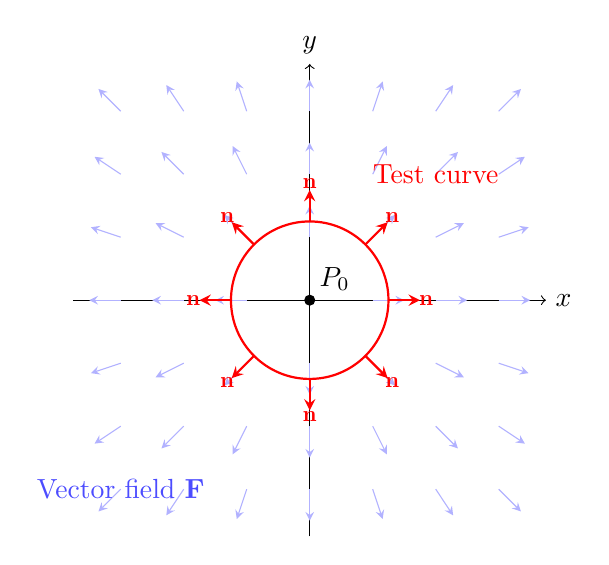
\begin{tikzpicture}[scale=2]
    % Draw axes
    \draw[->] (-1.5,0) -- (1.5,0) node[right] {$x$};
    \draw[->] (0,-1.5) -- (0,1.5) node[above] {$y$};
    
    % Draw source vector field (light)
    \foreach \x in {-1.2,-0.8,...,1.2} {
        \foreach \y in {-1.2,-0.8,...,1.2} {
            \pgfmathsetmacro{\len}{sqrt(\x*\x+\y*\y)}
            \pgfmathparse{\len > 0.1 ? 1 : 0}
            \if\pgfmathresult1
                \draw[-stealth, blue!30, thin] (\x,\y) -- 
                    +({0.2*\x/\len},{0.2*\y/\len});
            \fi
        }
    }
    
    % Draw test circle
    \draw[red, thick] (0,0) circle (0.5);
    
    % Draw normal vectors
    \foreach \angle in {0,45,...,315} {
        \draw[-stealth, red, thick] 
            ({0.5*cos(\angle)},{0.5*sin(\angle)}) -- 
            ({0.7*cos(\angle)},{0.7*sin(\angle)}) 
            node[pos=1.2, scale=0.8] {$\mathbf{n}$};
    }
    
    % Label center point P
    \fill (0,0) circle (1pt) node[above right] {$P_0$};
    
    % Add explanatory labels
    \node[red] at (0.8,0.8) {Test curve};
    \node[blue!70] at (-1.2,-1.2) {Vector field $\mathbf{F}$};
\end{tikzpicture}
\caption{\textit{To measure divergence at point $P_0$, we examine how much the vector field $\mathbf{F}$ flows across a small test curve (red). The outward unit normal vectors $\mathbf{n}$ help us measure the net outward flow.}}
\label{fig:divergence_probe}
\end{figure}
\index{Flux Integral}


\noindent At each point on our test curve, we can use the dot product $\mathbf{F} \cdot \mathbf{n}$ to measure how much the field flows outward (where $\mathbf{n}$ is the outward unit normal vector). Positive values indicate outward flow, negative values indicate inward flow. The line integral of this outward flux along our curve ($ds$ denoting infinitesimal arc length) gives us the total net outward flow:
\[
\oint_{C_r} \mathbf{F} \cdot \mathbf{n}\,ds
\]

\noindent Similar to our development of curl, if we want to measure the ``flow per unit area", we should divide by the area enclosed by our curve:
\[
\frac{1}{\pi r^2} \oint_{C_r} \mathbf{F} \cdot \mathbf{n}\,ds
\]

\noindent This ratio gives us profound insight into the field's behavior. Consider what happens if we shrink our test circle, making $r$ approach zero:
\[
\lim_{r \to 0} \frac{1}{\pi r^2} \oint_{C_r} \mathbf{F} \cdot \mathbf{n}\,ds
\]

\noindent This limit measures the pure expansive tendency at point $P_0$ - in fluid dynamics, it would tell us whether fluid is being created (positive divergence) or destroyed (negative divergence) at that point. For an incompressible fluid like water, this divergence must be zero everywhere - you can't create or destroy water in the flow! \\

\begin{figure}[H]
\centering
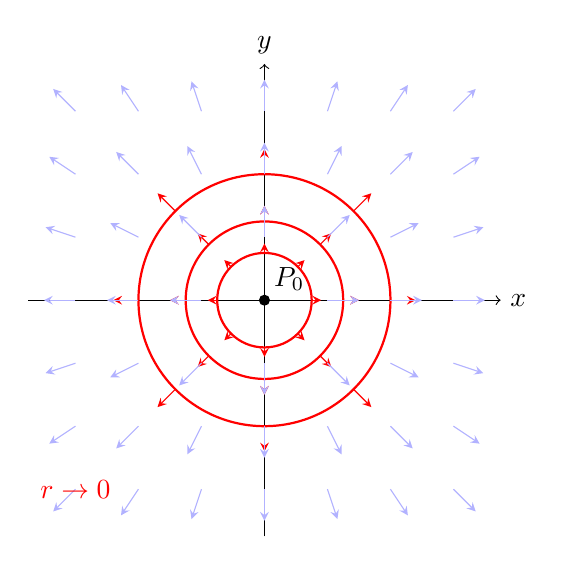
\begin{tikzpicture}[scale=2]
   % Draw axes
   \draw[->] (-1.5,0) -- (1.5,0) node[right] {$x$};
   \draw[->] (0,-1.5) -- (0,1.5) node[above] {$y$};
   
   % Draw three nested circles with normal vectors
   \foreach \rad in {0.8,0.5,0.3} {
       \draw[red, thick] (0,0) circle (\rad);
       \foreach \angle in {0,45,...,315} {
           \draw[-stealth, red, thin] 
               ({\rad*cos(\angle)},{\rad*sin(\angle)}) -- 
               ({1.2*\rad*cos(\angle)},{1.2*\rad*sin(\angle)});
       }
   }
   
   % Draw source field vectors (light)
   \foreach \x in {-1.2,-0.8,...,1.2} {
       \foreach \y in {-1.2,-0.8,...,1.2} {
           \pgfmathsetmacro{\len}{sqrt(\x*\x+\y*\y)}
           \pgfmathparse{\len > 0.1 ? 1 : 0}
           \if\pgfmathresult1
               \draw[-stealth, blue!30, thin] (\x,\y) -- 
                   +({0.2*\x/\len},{0.2*\y/\len});
           \fi
       }
   }
   
   % Label center point P
   \fill (0,0) circle (1pt) node[above right] {$P_0$};
   
   % Add annotations
   \node[red] at (-1.2,-1.2) {$r \to 0$};
\end{tikzpicture}
\caption{\textit{As we shrink our test curve around $P_0$, we measure the local expansive tendency of the field. The normal vectors (red) measure outward flow at each point.}}
\label{fig:shrinking_divergence}
\end{figure}

\noindent Let's pull out another can of math whoop-ass to get our definition of divergence, starting with the aforementioned flux integral around a small circle $C_r$ centered at $P_0$:
\[
\oint_{C_r} \mathbf{F} \cdot \mathbf{n}\,ds
\]
\noindent In polar coordinates our unit normal vector from the origin is $\mathbf{n} = \langle \cos\theta,\sin\theta\rangle$. Thus we have:
\[
\mathbf{F} \cdot \mathbf{n} = P \cos\theta + Q \sin\theta
\]
Express $\mathbf{F}$ in terms of its components and expand to first order using Taylor Series expansion:
\[
\mathbf{F} \cdot \mathbf{n} \approx \left(P + \frac{\partial P}{\partial x} r \cos\theta + \frac{\partial P}{\partial y} r \sin\theta\right)\cos\theta + \left(Q + \frac{\partial Q}{\partial x} r \cos\theta + \frac{\partial Q}{\partial y} r \sin\theta\right)\sin\theta
\]
Integrate over the circle and retain the leading terms:
\[
\oint_{C_r} \mathbf{F} \cdot \mathbf{n}\,ds \approx \pi r^2 \left( \frac{\partial P}{\partial x} + \frac{\partial Q}{\partial y} \right)
\]
Divide by the area $\pi r^2$ and take the limit as $r \to 0$:
\[
\lim_{r \to 0} \frac{1}{\pi r^2} \oint_{C_r} \mathbf{F} \cdot \mathbf{n}\,ds = \frac{\partial P}{\partial x} + \frac{\partial Q}{\partial y} = \nabla \cdot \mathbf{F}
\]
\[
\text{div }\mathbf{F} = \nabla \cdot \mathbf{F} = \frac{\partial P}{\partial x} + \frac{\partial Q}{\partial y}
\]

\noindent The physical interpretation is striking: $\frac{\partial P}{\partial x}$ measures how much the horizontal component changes as we move horizontally, while $\frac{\partial Q}{\partial y}$ measures how much the vertical component changes as we move vertically. Their sum tells us the total spreading out of the field at that point. \\

%https://tikz.net/curl/     Izaak Neutelings
\begin{figure}[H]
\centering
\colorlet{veccol}{orange!90!black}
\colorlet{myblue}{blue!60!black}
\tikzstyle{vector}=[->,thick,veccol]
\def\R{1.4}
\def\r{0.03}
\def\N{9}
\def\null{\color{myblue}{0}}

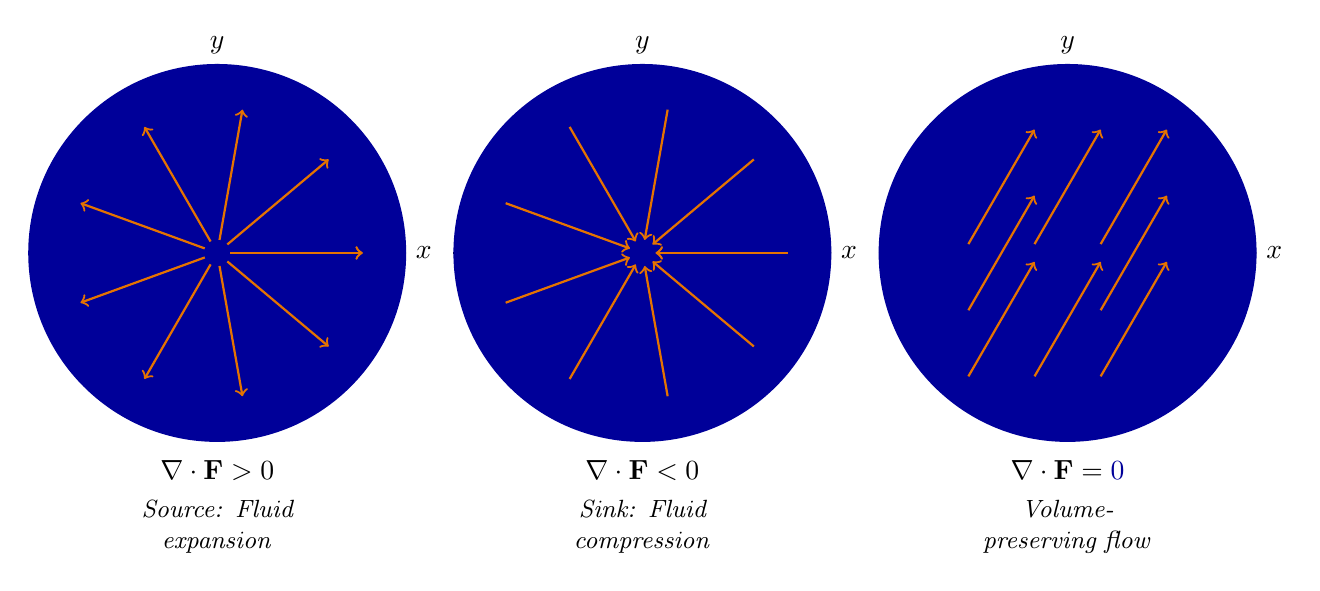
\begin{tikzpicture}[scale=1.2]
    % First diagram: Source field
    \begin{scope}[xshift=-4.5cm]
        % Axes
        \draw[thin, ->] (-2,0) -- (2,0) node[right] {$x$};
        \draw[thin, ->] (0,-2) -- (0,2) node[above] {$y$};
        
        % Central point
        \fill[myblue] (0,0) circle (\r);
        
        % Radial vectors with consistent spacing
        \foreach \i [evaluate={\ang=\i*360/\N;}] in {0,...,\N}{
            \draw[vector] (\ang:0.1*\R) --++ (\ang:\R);
        }
        
        % Label with mathematical notation
        \node at (0,-2.3) {$\nabla \cdot \mathbf{F} > 0$};
        \node[text width=3cm, align=center, font=\small] at (0,-2.9) 
            {\textit{Source: Fluid expansion}};
    \end{scope}
    
    % Second diagram: Sink field
    \begin{scope}[xshift=0cm]
        % Axes
        \draw[thin, ->] (-2,0) -- (2,0) node[right] {$x$};
        \draw[thin, ->] (0,-2) -- (0,2) node[above] {$y$};
        
        % Central point
        \fill[myblue] (0,0) circle (\r);
        
        % Radial vectors pointing inward
        \foreach \i [evaluate={\ang=\i*360/\N;}] in {0,...,\N}{
            \draw[vector] (\ang:1.1*\R) -- (\ang:0.1*\R);
        }
        
        % Label with mathematical notation
        \node at (0,-2.3) {$\nabla \cdot \mathbf{F}  < 0$};
        \node[text width=3cm, align=center, font=\small] at (0,-2.9) 
            {\textit{Sink: Fluid compression}};
    \end{scope}
    
    % Third diagram: Incompressible flow
    \begin{scope}[xshift=4.5cm]
        % Axes
        \draw[thin, ->] (-2,0) -- (2,0) node[right] {$x$};
        \draw[thin, ->] (0,-2) -- (0,2) node[above] {$y$};
        
        % Central point
        \fill[myblue] (0,0) circle (\r);
        
        % Parallel flow pattern
        \def\ang{60}
        \foreach \x/\y in {-1/0,-1/1,0/1,1/1,1/0,-1/-1,0/-1,1/-1}{
            \draw[vector] (\x*0.5*\R,\y*0.5*\R) ++ (\ang-180:\R/2) --++ (\ang:\R);
        }
        
        % Label with mathematical notation
        \node at (0,-2.3) {$\nabla \cdot \mathbf{F}  = \null$};
        \node[text width=3cm, align=center, font=\small] at (0,-2.9) 
            {\textit{Volume-preserving flow}};
    \end{scope}
\end{tikzpicture}
\caption{\textit{Fundamental divergence patterns in vector fields. The divergence measures the net flux per unit area. Left: A source field exhibits positive divergence as vectors emanate outward, indicating fluid expansion. Center: A sink field shows negative divergence as vectors converge inward, representing compression. Right: An incompressible flow field maintains zero divergence, preserving volume as fluid moves. Note how the vector patterns visually represent the mathematical concept of divergence through their geometric arrangement.}}
\label{fig:divergence_patterns}
\end{figure}

\noindent In three dimensions, divergence maintains its scalar nature:
\[
\text{div }\mathbf{F} = \nabla \cdot \mathbf{F} = \frac{\partial P}{\partial x} + \frac{\partial Q}{\partial y} + \frac{\partial R}{\partial z}
\]

\exampleline
\begin{example}
In fluid dynamics, the velocity field of flow through a pipe often exhibits interesting divergence patterns. Consider the following velocity field modeling fluid flow near a constriction:
\[
\mathbf{F}(x,y,z) = (2x)\mathbf{i} + (-y)\mathbf{j} + (-z)\mathbf{k}
\]
Calculate the divergence of this field and explain what it reveals about the fluid flow.

\begin{solution}
This ain't too bad.
\begin{enumerate}
\item First, recall that in three dimensions:
\[
\text{div }\mathbf{F} = \nabla \cdot \mathbf{F} = \frac{\partial P}{\partial x} + \frac{\partial Q}{\partial y} + \frac{\partial R}{\partial z}
\]

\item For our velocity field:
\begin{align*}
\frac{\partial P}{\partial x} &= \frac{\partial}{\partial x}(2x) = 2 \\[0.5em]
\frac{\partial Q}{\partial y} &= \frac{\partial}{\partial y}(-y) = -1 \\[0.5em]
\frac{\partial R}{\partial z} &= \frac{\partial}{\partial z}(-z) = -1
\end{align*}

\item Therefore:
\[
\text{div }\mathbf{F} = 2 - 1 - 1 = 0
\]

\item This zero divergence tells us something profound about our flow:
\begin{itemize}
   \item The fluid is incompressible - no fluid is being created or destroyed
   \item This matches what we expect in a pipe constriction - as the fluid is squeezed inward in two directions, it must speed up in the third direction to maintain the same volume flow rate
\end{itemize}

\end{enumerate}

\begin{figure}[H]
\centering
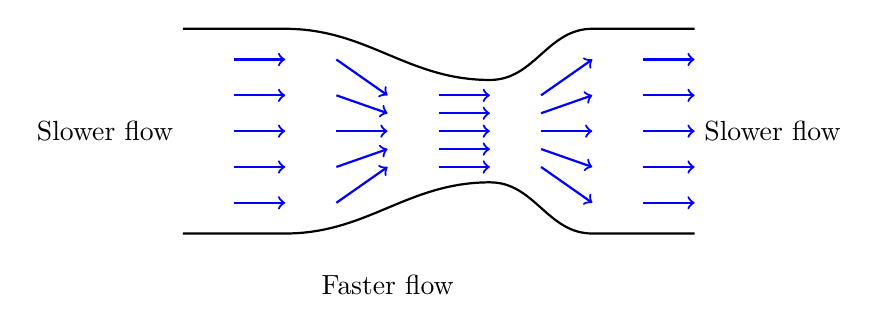
\begin{tikzpicture}[scale=1.3]
   % Draw pipe outline
   \draw[thick] (-2,1) -- (-1,1) to[out=0,in=180] (1,0.5)
                to[out=0,in=180] (2,1) -- (3,1);
   \draw[thick] (-2,-1) -- (-1,-1) to[out=0,in=180] (1,-0.5)
                to[out=0,in=180] (2,-1) -- (3,-1);
                
   % Draw flow lines with arrows
   \foreach \y in {-0.7,-0.35,0,0.35,0.7} {
       \draw[blue,->,thick] (-1.5,\y) -- (-1,\y);
       \draw[blue,->,thick] (-0.5,\y) -- (0,0.5*\y);
       \draw[blue,->,thick] (0.5,0.5*\y) -- (1,0.5*\y);
       \draw[blue,->,thick] (1.5,0.5*\y) -- (2,\y);
       \draw[blue,->,thick] (2.5,\y) -- (3,\y);
   }
   
   % Labels
   \node at (0,-1.5) {Faster flow};
   \node[left] at (-2,0) {Slower flow};
   \node[right] at (3,0) {Slower flow};
\end{tikzpicture}
\caption{\textit{The fluid speeds up where the pipe narrows (indicated by longer arrows) and slows down where it widens, maintaining constant volume throughout.}}
\label{fig:pipe_flow}
\end{figure}

\noindent This example illustrates a key principle in fluid dynamics: for an incompressible fluid, the divergence of the velocity field must be zero everywhere. In our case, the field automatically satisfies this condition through careful balance of its components.

\end{solution}
\end{example}
\exampleline

\subsection*{Vector Operators and Their Compositions} \index{Vector Operators}

\noindent We have now encountered three fundamental vector operators: the curl ($\nabla \times \mathbf{F} = \text{curl } \mathbf{F}$), divergence ($\nabla \cdot \mathbf{F} = \text{div } \mathbf{F}$), and from Chapter 3, the gradient of scalar functions ($\nabla f$, we will also notate this as $\text{grad } f$). The gradient, which we've also used implicitly in conservative fields converts a scalar field into a vector field by measuring the direction and magnitude of steepest increase:
\[
\text{grad }f = \nabla f = \frac{\partial f}{\partial x}\mathbf{i} + \frac{\partial f}{\partial y}\mathbf{j} + \frac{\partial f}{\partial z}\mathbf{k}
\]

\noindent These operators form a rich algebraic system with several remarkable properties:

\begin{itemize}
    \item \textbf{Curl of a Gradient}: For any scalar field $f$ (assuming sufficient smoothness),
    \[
    \text{curl}(\text{grad }f) = \nabla \times (\nabla f) = \mathbf{0}
    \]
    This explains why conservative fields (fields that are gradients) are always irrotational!

    \item \textbf{Divergence of a Curl}: For any vector field $\mathbf{F}$,
    \[
    \text{div}(\text{curl }\mathbf{F}) = \nabla \cdot (\nabla \times \mathbf{F}) = 0
    \]
    This means no matter how a field rotates, it never creates or destroys mass in doing so.
\index{Laplacian}
    \item \textbf{Second-order Compositions}: The Laplacian emerges when we take divergence of gradient:
    \[
    \text{div}(\text{grad }f) = \nabla \cdot (\nabla f) = \nabla^2f = \frac{\partial^2 f}{\partial x^2} + \frac{\partial^2 f}{\partial y^2} + \frac{\partial^2 f}{\partial z^2}
    \]
\end{itemize}

\noindent We have some intimate connections between Scalar Fields and Vector Fields that can be intertwined with these three operators:

\begin{figure}[H]
\centering
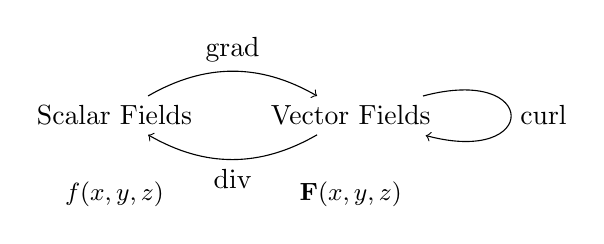
\begin{tikzpicture}[scale=2, node distance=3cm]
    % Create a diagram showing relationships
    \node (scalar) {Scalar Fields};
    \node[right of=scalar] (vector) {Vector Fields};
    
    % Draw arrows
    \draw[->] (scalar) to[bend left] node[above] {grad} (vector);
    \draw[->] (vector) to[bend left] node[below] {div} (scalar);
    \path[->] (vector) edge [loop right] node[right] {curl} (vector);
    
    % Add some notes
    \node[below of=scalar, yshift=2cm] {\small $f(x,y,z)$};
    \node[below of=vector, yshift=2cm] {\small $\mathbf{F}(x,y,z)$};
\end{tikzpicture}
\caption{\textit{The relationships between vector operators. Gradient maps scalar to vector fields, divergence does the reverse, and curl maps vector fields to vector fields.}}
\label{fig:vector_operators}
\end{figure}

\noindent Some key identities that often prove useful:

\begin{enumerate}
    \item For scalar fields $f$ and $g$:
    \[
    \nabla(fg) = f\nabla g + g\nabla f
    \]
    
    \item For a vector field $\mathbf{F}$:
    \[
    \nabla \cdot (f\mathbf{F}) = f(\nabla \cdot \mathbf{F}) + \mathbf{F} \cdot (\nabla f)
    \]
    
    \item The vector triple product:
    \[
    \nabla \times (\nabla \times \mathbf{F}) = \nabla(\nabla \cdot \mathbf{F}) - \nabla^2\mathbf{F}
    \]
\end{enumerate}

\noindent These relationships help explain many physical phenomena. For instance, Maxwell's equations in electromagnetics can be written elegantly using these operators:
\begin{itemize}
    \item $\nabla \cdot \mathbf{E} = \frac{\rho}{\epsilon_0}$ (Gauss's law)
    \item $\nabla \cdot \mathbf{B} = 0$ (No magnetic monopoles)
    \item $\nabla \times \mathbf{E} = -\frac{\partial \mathbf{B}}{\partial t}$ (Faraday's law)
    \item $\nabla \times \mathbf{B} = \mu_0\mathbf{J} + \mu_0\epsilon_0\frac{\partial \mathbf{E}}{\partial t}$ (Ampère's law)
\end{itemize}

\noindent The fact that $\nabla \cdot (\nabla \times \mathbf{F}) = 0$ ensures magnetic field lines always form closed loops (no magnetic monopoles), while $\nabla \times (\nabla f) = \mathbf{0}$ explains why electric fields in electrostatics can be written as the gradient of a potential.

\subsubsection*{FTOC Reformulated}

\noindent The Fundamental Theorem of Calculus can be extended naturally to parametric curves in higher dimensions. Given a scalar field $f$ and a curve $\mathbf{r}(t)$ for $a \leq t \leq b$, we can integrate the gradient along the curve to recover the total change in $f$:
\[
\int_C \nabla f \cdot d\mathbf{r} = f(\mathbf{r}(b)) - f(\mathbf{r}(a))
\]

\noindent This elegant formulation shows that for any curve, integrating the rate of change of a function along that curve yields the total change in the function. The geometric meaning becomes clear when we recall that $\nabla f$ points in the direction of steepest increase of $f$, and the dot product with $d\mathbf{r}$ measures how much we move in that direction. \\

\noindent Just as the original FTOC connected differentiation and integration in one dimension, this version connects them along any path through space—a profound generalization that bridges single-variable and multivariable calculus.

\exampleline
\begin{example}
Vector operator identities often prove useful in physics and engineering. Derive expressions for:
\begin{enumerate}
   \item $\nabla \cdot (\mathbf{F} \times \mathbf{G})$ where $\mathbf{F}$ and $\mathbf{G}$ are vector fields
   \item $\nabla \times (f\mathbf{F})$ where $f$ is a scalar field and $\mathbf{F}$ is a vector field
\end{enumerate}

\begin{solution}
\begin{enumerate}
\item For $\nabla \cdot (\mathbf{F} \times \mathbf{G})$:
\begin{itemize}
   \item Write $\mathbf{F} = F_1\mathbf{i} + F_2\mathbf{j} + F_3\mathbf{k}$ and $\mathbf{G} = G_1\mathbf{i} + G_2\mathbf{j} + G_3\mathbf{k}$
   
   \item The cross product is:
   \[
   \mathbf{F} \times \mathbf{G} = \begin{vmatrix} 
   \mathbf{i} & \mathbf{j} & \mathbf{k} \\
   F_1 & F_2 & F_3 \\
   G_1 & G_2 & G_3
   \end{vmatrix}
   \]
   \[
   = (F_2G_3 - F_3G_2)\mathbf{i} + (F_3G_1 - F_1G_3)\mathbf{j} + (F_1G_2 - F_2G_1)\mathbf{k}
   \]

   \item Take divergence:
   \begin{align*}
   \nabla \cdot (\mathbf{F} \times \mathbf{G}) &= \frac{\partial}{\partial x}(F_2G_3 - F_3G_2) + \frac{\partial}{\partial y}(F_3G_1 - F_1G_3) \\
   &\quad + \frac{\partial}{\partial z}(F_1G_2 - F_2G_1)
   \end{align*}

   \item Expand using product rule:
   \begin{align*}
   &= \left(\frac{\partial F_2}{\partial x}G_3 + F_2\frac{\partial G_3}{\partial x} - \frac{\partial F_3}{\partial x}G_2 - F_3\frac{\partial G_2}{\partial x}\right) \\
   &+ \left(\frac{\partial F_3}{\partial y}G_1 + F_3\frac{\partial G_1}{\partial y} - \frac{\partial F_1}{\partial y}G_3 - F_1\frac{\partial G_3}{\partial y}\right) \\
   &+ \left(\frac{\partial F_1}{\partial z}G_2 + F_1\frac{\partial G_2}{\partial z} - \frac{\partial F_2}{\partial z}G_1 - F_2\frac{\partial G_1}{\partial z}\right)
   \end{align*}

   \item Collect terms and recognize the dot product pattern:
   \[
   \nabla \cdot (\mathbf{F} \times \mathbf{G}) = \mathbf{G} \cdot (\nabla \times \mathbf{F}) - \mathbf{F} \cdot (\nabla \times \mathbf{G})
   \]
\end{itemize}

\item For $\nabla \times (f\mathbf{F})$:
\begin{itemize}
   \item Write out component-wise, using product rule:
   \begin{align*}
   \nabla \times (f\mathbf{F}) &= \begin{vmatrix}
   \mathbf{i} & \mathbf{j} & \mathbf{k} \\
   \frac{\partial}{\partial x} & \frac{\partial}{\partial y} & \frac{\partial}{\partial z} \\
   fF_1 & fF_2 & fF_3
   \end{vmatrix} \\[1em]
   &= \left(\frac{\partial}{\partial y}(fF_3) - \frac{\partial}{\partial z}(fF_2)\right)\mathbf{i} \\
   &+ \left(\frac{\partial}{\partial z}(fF_1) - \frac{\partial}{\partial x}(fF_3)\right)\mathbf{j} \\
   &+ \left(\frac{\partial}{\partial x}(fF_2) - \frac{\partial}{\partial y}(fF_1)\right)\mathbf{k}
   \end{align*}

   \item Apply product rule to each term:
   \begin{align*}
   \nabla \times (f\mathbf{F}) &= f(\nabla \times \mathbf{F}) + \nabla f \times \mathbf{F}
   \end{align*}
\end{itemize}

\end{enumerate}

\noindent These identities are particularly useful in fluid dynamics and electromagnetics. For example, in ideal fluid flow, the term $\nabla \times (f\mathbf{F})$ appears when studying vorticity transport, while $\nabla \cdot (\mathbf{F} \times \mathbf{G})$ arises in the study of helicity in fluid flows.

\end{solution}
\end{example}
\exampleline


\subsection*{Vector Operators in Different Coordinate Systems}

\noindent So far, we've worked exclusively in Cartesian coordinates, where our formulas for gradient, divergence, and curl took relatively simple forms. However, many physical problems are more naturally expressed in other coordinate systems. For instance, studying planetary motion is easier in spherical coordinates, while analyzing flow through a pipe often uses cylindrical coordinates. \\

\noindent Here's how our vector operators transform in common coordinate systems:

\begin{table}[H]
\centering
\begin{tabular}{|c|c|c|}
\hline
\textbf{Operator} & \textbf{Cylindrical} $(r,\theta,z)$ & \textbf{Spherical} $(r,\theta,\phi)$ \\
\hline
\rule{0pt}{4ex}
$\nabla f$ & $\displaystyle\frac{\partial f}{\partial r}\mathbf{e}_r + \frac{1}{r}\frac{\partial f}{\partial \theta}\mathbf{e}_\theta + \frac{\partial f}{\partial z}\mathbf{e}_z$ & $\displaystyle\frac{\partial f}{\partial r}\mathbf{e}_r + \frac{1}{r}\frac{\partial f}{\partial \theta}\mathbf{e}_\theta + \frac{1}{r\sin\theta}\frac{\partial f}{\partial \phi}\mathbf{e}_\phi$ \\[2ex]
\hline
\rule{0pt}{4ex}
$\nabla \cdot \mathbf{F}$ & $\displaystyle\frac{1}{r}\frac{\partial}{\partial r}(rF_r) + \frac{1}{r}\frac{\partial F_\theta}{\partial \theta} + \frac{\partial F_z}{\partial z}$ & $\displaystyle\frac{1}{r^2}\frac{\partial}{\partial r}(r^2F_r) + \frac{1}{r\sin\theta}\frac{\partial}{\partial \theta}(\sin\theta F_\theta) + \frac{1}{r\sin\theta}\frac{\partial F_\phi}{\partial \phi}$ \\[2ex]
\hline
\rule{0pt}{6ex}
$\nabla \times \mathbf{F}$ & $\begin{pmatrix} 
\frac{1}{r}\frac{\partial F_z}{\partial \theta} - \frac{\partial F_\theta}{\partial z} \\[1ex]
\frac{\partial F_r}{\partial z} - \frac{\partial F_z}{\partial r} \\[1ex]
\frac{1}{r}\frac{\partial}{\partial r}(rF_\theta) - \frac{1}{r}\frac{\partial F_r}{\partial \theta}
\end{pmatrix}$ & $\begin{pmatrix}
\frac{1}{r\sin\theta}\left(\frac{\partial}{\partial \theta}(\sin\theta F_\phi) - \frac{\partial F_\theta}{\partial \phi}\right) \\[1ex]
\frac{1}{r}\left(\frac{1}{\sin\theta}\frac{\partial F_r}{\partial \phi} - \frac{\partial}{\partial r}(rF_\phi)\right) \\[1ex]
\frac{1}{r}\left(\frac{\partial}{\partial r}(rF_\theta) - \frac{\partial F_r}{\partial \theta}\right)
\end{pmatrix}$ \\[6ex]
\hline
\end{tabular}
\caption{\textit{Vector operators in cylindrical and spherical coordinates. Note how factors of $r$ and $\sin\theta$ appear to account for the geometry.}}
\label{tab:coord_operators}
\end{table}

\noindent These expressions might look intimidating, but they arise naturally from the geometry of these coordinate systems. For instance, the factor of $\frac{1}{r}$ in cylindrical coordinates accounts for the fact that the length of a circular arc increases with radius. Similarly, the $\sin\theta$ terms in spherical coordinates reflect the convergence of longitude lines at the poles. \\

\noindent One particularly useful fact: the expressions for divergence ensure that Gauss's theorem works in any coordinate system—the divergence always represents the flux per unit volume, regardless of how we measure that volume.

\exampleline
\begin{example}
The electric field due to an infinite straight wire carrying current $I$ is given in cylindrical coordinates by:
\[
\mathbf{E}(r,\theta,z) = \frac{k}{r}\mathbf{e}_r
\]
where $k$ is a constant. Verify that this field is irrotational (curl-free) and compute its divergence.

\begin{solution}
Let's approach this systematically using our cylindrical coordinate formulas:

\begin{enumerate}
\item First, let's identify our components:
\[
E_r = \frac{k}{r}, \quad E_\theta = 0, \quad E_z = 0
\]

\item To compute curl $\mathbf{E}$, we need all three components:
\begin{align*}
(\nabla \times \mathbf{E})_r &= \frac{1}{r}\frac{\partial E_z}{\partial \theta} - \frac{\partial E_\theta}{\partial z} = 0 \\[1em]
(\nabla \times \mathbf{E})_\theta &= \frac{\partial E_r}{\partial z} - \frac{\partial E_z}{\partial r} = 0 \\[1em]
(\nabla \times \mathbf{E})_z &= \frac{1}{r}\frac{\partial}{\partial r}(rE_\theta) - \frac{1}{r}\frac{\partial E_r}{\partial \theta} = 0
\end{align*}
Therefore, $\nabla \times \mathbf{E} = \mathbf{0}$, confirming the field is irrotational.

\item For divergence:
\begin{align*}
\nabla \cdot \mathbf{E} &= \frac{1}{r}\frac{\partial}{\partial r}(rE_r) + \frac{1}{r}\frac{\partial E_\theta}{\partial \theta} + \frac{\partial E_z}{\partial z} \\[1em]
&= \frac{1}{r}\frac{\partial}{\partial r}\left(k\right) + 0 + 0 \\[1em]
&= 0
\end{align*}
\end{enumerate}

\noindent The zero divergence everywhere except at $r=0$ (where the field is undefined) tells us this is a valid solution to Laplace's equation in free space. This matches what we expect for an electric field in a region with no charges. The irrotational nature confirms that this field can be written as the gradient of a scalar potential.

\end{solution}
\end{example}
\exampleline



\newpage

\lecture{Surface Integrals}  \index{Surface Integrals}

\noindent Surface integrals are the natural evolution of mathematical curiosity—because apparently, integrating along lines wasn’t ambitious enough. While line integrals let us accumulate quantities along a path, surface integrals take things up a notch by summing contributions across two-dimensional surfaces in three-dimensional space. Useful, if you’ve ever found yourself pondering electromagnetic fields, fluid flow through membranes, or heat transfer across boundaries during your morning tea. 

\subsection*{Parameterized Surfaces} \index{Parametric Surfaces}

\noindent Consider the humble soap bubble, floating serenely until my toddler son Andy, an agent of chaos, pokes it with unbridled enthusiasm, leaving only a fleeting memory and some soapy residue. The bubble’s surface—its tension, the way it reflects light, and the air flowing around it—offers a wealth of complexity. Mathematically, analyzing such phenomena requires surface integrals. These integrals come in two flavors: those measuring accumulation over a surface and those measuring flow through a surface (like calculating how much water trickles through a filter). And there you have it: bubbles, toddlers, and integrals, all proving that life’s simplest joys can also be mind-bendingly complicated. \\

\noindent Recall that a parametric curve in space is given by a vector-valued function of one parameter:
\[
\mathbf{r}(t) = x(t)\mathbf{i} + y(t)\mathbf{j} + z(t)\mathbf{k}
\]
As $t$ varies, this function traces out a one-dimensional path through space. The single parameter $t$ gives us freedom to move in one dimension—along the curve. To describe a surface, we need more freedom of movement. We need to be able to move in two independent directions at any point. This naturally leads us to functions of two parameters:
\[
\mathbf{r}(u,v) = x(u,v)\mathbf{i} + y(u,v)\mathbf{j} + z(u,v)\mathbf{k}
\]

\noindent Think of $u$ and $v$ as coordinates on a ``parameter plane". Each point $(u,v)$ in this plane maps to a point on our surface in three-dimensional space. As we vary both parameters, we sweep out a two-dimensional surface rather than a one-dimensional curve. \\

\begin{figure}[H]
\centering
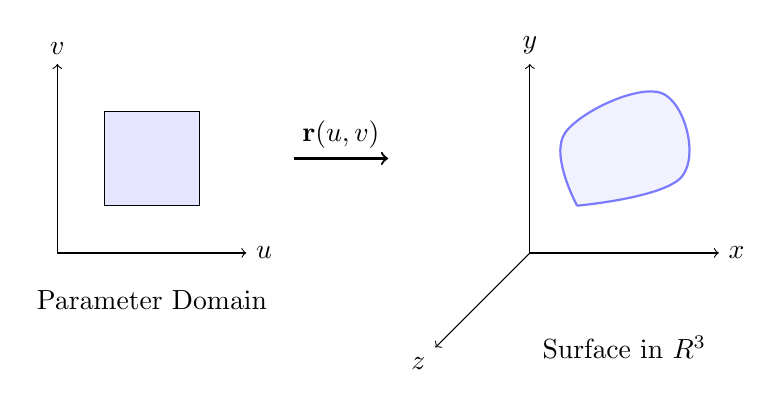
\begin{tikzpicture}[scale=1.2]
    % Parameter plane (uv-plane)
    \begin{scope}[xshift=-3cm]
        \draw[->] (0,0) -- (2,0) node[right] {$u$};
        \draw[->] (0,0) -- (0,2) node[above] {$v$};
        \draw[fill=blue!10] (0.5,0.5) rectangle (1.5,1.5);
        \node at (1,-0.5) {Parameter Domain};
    \end{scope}
    
    % 3D space
    \begin{scope}[xshift=2cm]
        \draw[->] (0,0) -- (2,0) node[right] {$x$};
        \draw[->] (0,0) -- (0,2) node[above] {$y$};
        \draw[->] (0,0) -- (-1,-1) node[below left] {$z$};
        \draw[blue, thick, fill=blue!10, opacity=0.5] 
            plot[smooth, tension=0.7] coordinates 
            {(0.5,0.5,0) (1.5,0.7,-0.3) (1.2,1.5,-0.5) (0.3,1.2,-0.2) (0.5,0.5,0)};
        \node at (1,-1) {Surface in $\mathbb{R}^3$};
    \end{scope}
    
    % Mapping arrow
    \draw[->, thick] (-0.5,1) -- (0.5,1) node[midway,above] {$\mathbf{r}(u,v)$};
\end{tikzpicture}
\caption{\textit{The parametric mapping $\mathbf{r}(u,v)$ transforms regions in the parameter plane to pieces of surface in three-dimensional space.}}
\label{fig:parameter_mapping}
\end{figure}

\noindent When working with surfaces, we often need to convert between parametric and scalar representations. Moving from parametric to scalar form involves writing out how $x$, $y$, and $z$ depend on parameters, then systematically eliminating those parameters through substitution and algebra. We must carefully track any parameter restrictions as these become domain constraints in our final scalar equation. Let's see some examples:


\exampleline
\begin{example}
Let’s practice converting between parametric and scalar representations of surfaces. These problems progress in difficulty, with the last one presenting a more intricate challenge.

\begin{enumerate}
\item Convert the parametric surface
\[
\mathbf{r}(u,v) = (u\cos v)\mathbf{i} + (u\sin v)\mathbf{j} + u\mathbf{k}
\]
where $u \geq 0$ and $0 \leq v \leq 2\pi$, to scalar form.

\item Convert the parametric surface
\[
\mathbf{r}(u,v) = (\sinh u \cos v)\mathbf{i} + (\sinh u \sin v)\mathbf{j} + (\cosh u)\mathbf{k}
\]
where $u \geq 0$ and $0 \leq v \leq 2\pi$, to scalar form.

\item Convert the parametric surface
\[
\mathbf{r}(u,v) = \left(u\sqrt{1-v^2}\right)\mathbf{i} + \left(uv\right)\mathbf{j} + \left(\frac{1}{1-v^2}\right)\mathbf{k}
\]
where $-1 < v < 1$ and $u > 0$, to scalar form.
\end{enumerate}

\begin{solution}
\begin{enumerate}
\item For the first parametric surface:
   \begin{itemize}
       \item The component equations are:
       \begin{align*}
           x &= u \cos v \\
           y &= u \sin v \\
           z &= u
       \end{align*}

       \item Square and add the $x$ and $y$ equations to eliminate $v$:
       \[
       x^2 + y^2 = u^2 (\cos^2 v + \sin^2 v) = u^2
       \]

       \item Since $z = u$, the scalar equation is:
       \[
       x^2 + y^2 = z^2
       \]
       The domain constraint is $z \geq 0$ since $u \geq 0$.
   \end{itemize}

\item For the second parametric surface:
   \begin{itemize}
       \item The component equations are:
       \begin{align*}
           x &= \sinh u \cos v \\
           y &= \sinh u \sin v \\
           z &= \cosh u
       \end{align*}

       \item Square and add the $x$ and $y$ equations to eliminate $v$:
       \[
       x^2 + y^2 = \sinh^2 u (\cos^2 v + \sin^2 v) = \sinh^2 u
       \]

       \item Use the hyperbolic identity $\cosh^2 u - \sinh^2 u = 1$ to express $\sinh^2 u$ in terms of $z$:
       \[
       x^2 + y^2 = \cosh^2 u - 1 = z^2 - 1
       \]

       \item The scalar equation is:
       \[
       x^2 + y^2 + 1 = z^2
       \]
       The domain constraint is $z \geq 1$ since $u \geq 0$.
   \end{itemize}

\item For the third parametric surface:
   \begin{itemize}
       \item The component equations are:
       \begin{align*}
           x &= u \sqrt{1 - v^2} \\
           y &= u v \\
           z &= \frac{1}{1 - v^2}
       \end{align*}

       \item Solve for $u$ in terms of $x$ and $v$:
       \[
       u = \frac{x}{\sqrt{1 - v^2}}
       \]

       \item Substitute $u$ into $y = u v$:
       \[
       y = \frac{x v}{\sqrt{1 - v^2}}
       \]

       \item Solve for $v^2$ in terms of $z$ using the third equation:
       \[
       z = \frac{1}{1 - v^2} \quad \Rightarrow \quad 1 - v^2 = \frac{1}{z} \quad \Rightarrow \quad v^2 = 1 - \frac{1}{z}
       \]
       Note: Since $-1 < v < 1$ and $u > 0$, we have $z \geq 1$.

       \item Substitute $v^2 = 1 - \frac{1}{z}$ into the equation for $y$:
       \[
       y = \frac{x v}{\sqrt{1 - v^2}} = \frac{x v}{\sqrt{\frac{1}{z}}} = x v \sqrt{z}
       \]
       Since $v^2 = 1 - \frac{1}{z}$, we have:
       \[
       v = \pm \sqrt{1 - \frac{1}{z}}
       \]
       Therefore:
       \[
       y = \pm x \sqrt{z} \sqrt{1 - \frac{1}{z}} = \pm x \sqrt{z \left(1 - \frac{1}{z}\right)} = \pm x \sqrt{z - 1}
       \]

       \item Square both sides to eliminate the square root and the sign:
       \[
       y^2 = x^2 (z - 1)
       \]

       \item Rearrange to obtain the scalar equation:
       \[
       x^2 z - x^2 - y^2 = 0
       \]
       Or, equivalently:
       \[
       x^2 z = x^2 + y^2
       \]
       
       Domain Constraint:
       \[
       z \geq 1
       \]
   \end{itemize}
\end{enumerate}
\end{solution}
\end{example}
\exampleline


\noindent Moving from scalar to parametric form requires choosing appropriate parameters based on the surface's geometry. For explicit surfaces, we often use $x, y$ as parameters directly. For cylindrical surfaces, parameters such as height and angle are more appropriate, while spherical coordinates are typically used for spherical surfaces. After selecting the parameters, the coordinates are expressed in terms of these parameters, and their ranges are determined to ensure proper coverage of the surface. \\

\noindent Common strategies for parameterization include the following:
\begin{itemize}
    \item \textbf{Level Curve Method:} This method involves holding one variable constant (e.g., $z$ in the surface $z = f(x, y)$) to obtain level curves. These curves represent intersections of the surface with horizontal planes and can be parameterized independently. The parameters are then combined to describe the entire surface.
    \item \textbf{Trace Method:} This method examines the intersections of the surface with planes parallel to coordinate planes, such as $x = c$ or $y = c$. Each intersection results in a curve (called a trace) that can be parameterized. By varying the fixed variable and combining the parameterizations, we obtain the parametric form of the surface.
    \item \textbf{Direct Substitution:} For explicitly defined surfaces (e.g., $z = f(x, y)$), $x$ and $y$ can be used directly as parameters, and $z$ is computed from the surface equation.
\end{itemize}


\noindent For the latter, here are some basic forms of parameterization:

\begin{enumerate}
    \item For $x = f(y,z)$: Use $y,z$ as parameters
    \[
    \mathbf{r}(y,z) = f(y,z)\mathbf{i} + y\mathbf{j} + z\mathbf{k}
    \]
    
    \item For $y = f(x,z)$: Use $x,z$ as parameters
    \[
    \mathbf{r}(x,z) = x\mathbf{i} + f(x,z)\mathbf{j} + z\mathbf{k}
    \]
    
    \item For $z = f(x,y)$: Use $x,y$ as parameters
    \[
    \mathbf{r}(x,y) = x\mathbf{i} + y\mathbf{j} + f(x,y)\mathbf{k}
    \]
\end{enumerate}

\noindent These forms are particularly useful when our surface is given by an equation that can be solved for one variable.

\exampleline
\begin{example}
Let's explore three fundamental techniques for working with surface representations. These problems demonstrate the key strategies for converting between parametric and scalar forms.

\begin{enumerate}
\item Convert the scalar surface $x^2 + y^2 = 4z^2$ to parametric form using the \textbf{level curve method}.

\item Convert the elliptic paraboloid $x = 5y^2 + 2z^2 - 10$ to parametric form using the \textbf{trace method}, considering only the portion in front of the $yz$-plane (where $x \geq 0$).
\end{enumerate}

\begin{solution}
\begin{enumerate}
\item For the cone $x^2 + y^2 = 4z^2$ (using the \textbf{level curve method}):
   \begin{itemize}
       \item Consider fixing $z = c$, which gives a circle in the $x, y$-plane:
       \[
       x^2 + y^2 = 4c^2
       \]

       \item Parameterize the level curve as:
       \[
       x = 2z\cos\theta, \quad y = 2z\sin\theta
       \]

       \item Combine the parameterization with the variable $z$:
       \[
       \mathbf{r}(z,\theta) = (2z\cos\theta)\mathbf{i} + (2z\sin\theta)\mathbf{j} + z\mathbf{k}
       \]
       where $z \in \mathbb{R}$ and $0 \leq \theta \leq 2\pi$.
   \end{itemize}

\item For the elliptic paraboloid $x = 5y^2 + 2z^2 - 10$ (using the \textbf{trace method}):
   \begin{itemize}
       \item Consider fixing $y = c$, which gives a parabola in the $xz$-plane:
       \[
       x = 5c^2 + 2z^2 - 10
       \]

       \item Parameterize $x$ in terms of $y$ and $z$:
       \[
       \mathbf{r}(y,z) = (5y^2 + 2z^2 - 10)\mathbf{i} + y\mathbf{j} + z\mathbf{k}
       \]

       \item The domain is constrained by $x \geq 0$, which implies:
       \[
       5y^2 + 2z^2 \geq 10 \quad \text{or equivalently} \quad \frac{y^2}{2} + \frac{z^2}{5} \geq 1
       \]
   \end{itemize}
\end{enumerate}

\noindent Note how each solution leverages different geometric insights: circular level curves in problem 1 and parabolic traces in problem 2. The choice of parameterization emerges naturally from each surface's inherent geometric properties.

\end{solution}
\end{example}
\exampleline

\begin{example}
Many of the most beautiful and practically important surfaces in mathematics and physics cannot be written as $z = f(x,y)$. Here we construct parametric representations of three such surfaces from their geometric descriptions.

\begin{enumerate}
\item \textbf{The Torus.} A torus (donut shape) is formed by revolving a circle of radius $a$ around the $z$-axis at distance $R$ from the center of the circle ($R > a$). Find a parametric representation.

\item \textbf{The Helicoid.} A helicoid is the surface swept out by a horizontal line segment that simultaneously rotates about the $z$-axis and translates upward along it at constant rates---think of a spiral staircase or a drill bit. If the segment has length $2$ and the surface rises by $2\pi c$ per full revolution, parameterize the helicoid.

\item \textbf{The Möbius Strip.} Take a strip of paper, give it a half-twist, and glue the ends together. Parameterize this surface.
\end{enumerate}

\begin{solution}
\begin{enumerate}
\item \textbf{The Torus.}

We need two parameters: $u \in [0, 2\pi]$ to revolve around the $z$-axis (the ``big" circle through the hole), and $v \in [0, 2\pi]$ to travel around the tube (the ``small" circle of the cross-section).

At angle $v$ around the tube, a point on the circle of radius $a$ sits at distance $R + a\cos v$ from the $z$-axis and at height $a\sin v$. Revolving this point around the $z$-axis by angle $u$ gives:
\[
\mathbf{r}(u,v) = (R + a\cos v)\cos u\,\mathbf{i} + (R + a\cos v)\sin u\,\mathbf{j} + a\sin v\,\mathbf{k}
\]

\textit{Verification:} When $v = 0$, the point is at distance $R + a$ from the $z$-axis (outer equator). When $v = \pi$, the distance is $R - a$ (inner equator). To find the scalar equation, observe that $\sqrt{x^2 + y^2} = R + a\cos v$ and $z = a\sin v$, so:
\[
\left(\sqrt{x^2 + y^2} - R\right)^2 + z^2 = a^2\cos^2 v + a^2\sin^2 v = a^2
\]

\item \textbf{The Helicoid.}

Let $u \in [-1, 1]$ parameterize position along the line segment, and let $v$ be the angle of rotation. At angle $v$, the segment points in the horizontal direction $\langle \cos v, \sin v, 0 \rangle$ and has risen to height $z = cv$. A point at position $u$ along the segment is therefore:
\[
\mathbf{r}(u,v) = u\cos v\,\mathbf{i} + u\sin v\,\mathbf{j} + cv\,\mathbf{k}
\]
where $u \in [-1, 1]$ and $v \in [0, 2\pi]$ for one full turn (extend $v$ further for additional turns).

This is a \textit{ruled surface}: for each fixed $v$, the map $u \mapsto \mathbf{r}(u,v)$ traces a straight line. Remarkably, the helicoid is also a \textit{minimal surface}---it locally minimizes surface area, just like a soap film spanning a wire frame. It is, in fact, the only ruled minimal surface besides the plane.

\item \textbf{The Möbius Strip.}

Start with a centerline circle of radius $R$ in the $xy$-plane, parameterized by $u \in [0, 2\pi]$. At each point on this circle, attach a short line segment of half-width $w$ that tilts out of the $xy$-plane by angle $u/2$---the half-twist:
\[
\mathbf{r}(u,v) = \left(R + v\cos\frac{u}{2}\right)\cos u\,\mathbf{i} + \left(R + v\cos\frac{u}{2}\right)\sin u\,\mathbf{j} + v\sin\frac{u}{2}\,\mathbf{k}
\]
where $u \in [0, 2\pi]$ and $v \in [-w, w]$ (e.g., $w = 0.5$).

The key is the $u/2$ in the tilt angles: after one full revolution ($u = 0$ to $u = 2\pi$), the strip has rotated by only $\pi$---a half-twist. The ``top" and ``bottom" edges swap, giving the Möbius strip its famous property of having only \textbf{one side}. This non-orientability means you cannot consistently define an outward normal vector on the entire surface, which has profound consequences: Stokes' Theorem requires an orientable surface, so it cannot be applied to a Möbius strip.
\end{enumerate}
\end{solution}
\end{example}
\exampleline

\begin{example}
The choice of parameterization determines how you compute with a surface. The same surface can look very different depending on which parameters you use, and some parameterizations are better suited to particular computations.

\begin{enumerate}
\item Parameterize the sphere $x^2 + y^2 + z^2 = a^2$ in three different ways: (a) using spherical coordinates, (b) using cylindrical coordinates, and (c) as a graph.

\item Using the spherical parameterization, compute the normal vector $\mathbf{r}_\theta \times \mathbf{r}_\phi$ and verify it points radially.
\end{enumerate}

\begin{solution}
\begin{enumerate}
\item Three parameterizations of the sphere:

\textbf{(a) Spherical coordinates.} Let $\phi \in [0, \pi]$ be the polar angle measured from the positive $z$-axis and $\theta \in [0, 2\pi]$ be the azimuthal angle:
\[
\mathbf{r}(\theta, \phi) = a\sin\phi\cos\theta\,\mathbf{i} + a\sin\phi\sin\theta\,\mathbf{j} + a\cos\phi\,\mathbf{k}
\]
This covers the entire sphere. At the poles ($\phi = 0$ or $\pi$), all values of $\theta$ map to the same point (the parameterization degenerates), but this causes no difficulty in practice.

\textbf{(b) Cylindrical coordinates.} From the sphere equation, $r = \sqrt{a^2 - z^2}$, so using $\theta \in [0, 2\pi]$ and $z \in [-a, a]$:
\[
\mathbf{r}(\theta, z) = \sqrt{a^2 - z^2}\cos\theta\,\mathbf{i} + \sqrt{a^2 - z^2}\sin\theta\,\mathbf{j} + z\,\mathbf{k}
\]
This also covers the entire sphere but degenerates at the poles ($z = \pm a$, where $r = 0$). This form is useful when the integrand depends naturally on $z$.

\textbf{(c) As a graph.} For the upper hemisphere, $z = \sqrt{a^2 - x^2 - y^2}$ over the disk $x^2 + y^2 \leq a^2$:
\[
\mathbf{r}(x,y) = x\,\mathbf{i} + y\,\mathbf{j} + \sqrt{a^2 - x^2 - y^2}\,\mathbf{k}
\]
This covers only a hemisphere and degenerates at the equator where the square root vanishes. Its simplicity makes it ideal for quick computations, but you need two such patches (upper and lower) for the full sphere.

\item Computing the normal from spherical coordinates:
\begin{align*}
\mathbf{r}_\theta &= -a\sin\phi\sin\theta\,\mathbf{i} + a\sin\phi\cos\theta\,\mathbf{j} + 0\,\mathbf{k} \\
\mathbf{r}_\phi &= a\cos\phi\cos\theta\,\mathbf{i} + a\cos\phi\sin\theta\,\mathbf{j} - a\sin\phi\,\mathbf{k}
\end{align*}

Their cross product:
\begin{align*}
\mathbf{r}_\theta \times \mathbf{r}_\phi &= \begin{vmatrix} \mathbf{i} & \mathbf{j} & \mathbf{k} \\ -a\sin\phi\sin\theta & a\sin\phi\cos\theta & 0 \\ a\cos\phi\cos\theta & a\cos\phi\sin\theta & -a\sin\phi \end{vmatrix} \\
&= -a^2\sin^2\phi\cos\theta\,\mathbf{i} - a^2\sin^2\phi\sin\theta\,\mathbf{j} - a^2\sin\phi\cos\phi\,\mathbf{k} \\
&= -a\sin\phi\underbrace{\left(a\sin\phi\cos\theta\,\mathbf{i} + a\sin\phi\sin\theta\,\mathbf{j} + a\cos\phi\,\mathbf{k}\right)}_{\mathbf{r}(\theta,\phi)}
\end{align*}

Since $\sin\phi \geq 0$ for $\phi \in [0,\pi]$, this points \textit{inward} (opposite to $\mathbf{r}$). For the \textbf{outward} normal, reverse the order: $\mathbf{r}_\phi \times \mathbf{r}_\theta = a\sin\phi\,\mathbf{r}$. Its magnitude is $\|\mathbf{r}_\phi \times \mathbf{r}_\theta\| = a^2\sin\phi$, yielding the familiar surface area element $dS = a^2\sin\phi\,d\theta\,d\phi$ for spherical coordinates---which integrates to $4\pi a^2$, the surface area of a sphere.
\end{enumerate}
\end{solution}
\end{example}
\exampleline


\subsection*{Tangent Planes and Surface Normal}

\noindent At each point on our surface, we can move in two independent directions, determined by our parameters $u$ and $v$. When we vary $u$ slightly (keeping $v$ fixed), we move in the direction of:
\[
\mathbf{r}_u = \frac{\partial \mathbf{r}}{\partial u} = \frac{\partial x}{\partial u}\mathbf{i} + \frac{\partial y}{\partial u}\mathbf{j} + \frac{\partial z}{\partial u}\mathbf{k}
\]

\noindent Similarly, varying $v$ (keeping $u$ fixed) moves us in the direction:
\[
\mathbf{r}_v = \frac{\partial \mathbf{r}}{\partial v} = \frac{\partial x}{\partial v}\mathbf{i} + \frac{\partial y}{\partial v}\mathbf{j} + \frac{\partial z}{\partial v}\mathbf{k}
\]

\noindent These vectors $\mathbf{r}_u$ and $\mathbf{r}_v$ are tangent to the surface and span the tangent plane at each point. Their cross product:
\[
\mathbf{n} = \mathbf{r}_u \times \mathbf{r}_v
\]
gives us a vector normal to the surface which we can use to construct the plane equation. \\

\begin{figure}[H]
\centering
\begin{tikzpicture}[line cap=round,line join=round,3d view={110}{20},scale=1.5]
% dimensions
\def\r{2}    % sphere radius
\def\c{0.5}  % center C position
\def\cx{0.5} % curve x position
\pgfmathsetmacro\ra{sqrt(\r*\r-\c*\c)}             % radius, arcs in the sphere
\pgfmathsetmacro\rc{sqrt(\r*\r-(\c+\cx)*(\c+\cx))} % radius, curve
\pgfmathsetmacro\axy{asin(\c/\r)}                  % angles in xy plane
\pgfmathsetmacro\ayz{asin(\c/\ra)}                 % angles in yz plane 
\pgfmathsetmacro\ar{asin((\c+\cx)/\r}              % rotation angle for plane and vectors
% coordinates
\coordinate (C) at (-\c,\c,0); % sphere center
\coordinate (O) at (0,0,0);
\coordinate (P) at (\cx,\c,{sqrt(\r*\r-(\c+\cx)*(\c+\cx))});
\coordinate (G) at ($(C)!1.7!(P)$); % gradient
\coordinate (RU) at (1, 0, 0);
\coordinate (RV) at (0, 1, 0);
% some auxiliary lines
%\begin{scope}[gray,very thin]
%  \draw (C) circle (\r cm);
%  \draw (C) --++   (\r,0,0);
%  \draw[canvas is xy plane at z=0]      (C) circle (\r);
%  \draw[canvas is xz plane at y=0]  (-\c,0) circle (\ra);
%  \draw[canvas is yz plane at x=0]   (\c,0) circle (\ra);
%  \draw[canvas is yz plane at x=\cx] (\c,0) circle (\rc);
%\end{scope}
% axes
\draw[-latex] (O) -- (\r+1,0,0) node[left]  {$x$};
\draw[-latex] (O) -- (0,\r+1,0) node[right] {$y$};
\draw[-latex] (O) -- (0,0,\r+1) node[above] {$z$};
% surface
\draw[surface] (C) ++ (-\axy:\r) arc (-\axy:90-\axy:\r)
    {[canvas is yz plane at x=0] arc (0:90+\ayz:\ra)}
    {[canvas is xz plane at y=0] arc (90-\ayz:0:\ra)};
% curve
\draw[canvas is yz plane at x=\cx,yellow] (\c+\rc,0) arc (0:{90+asin(\c/\rc)}:\rc);
% plane
\draw[plane,shift={(P)},rotate around y=\ar,canvas is xy plane at z=0] (-1,-1.5) -|++ (2,3) -| cycle;
% Point P
\fill (P) circle (0.4mm) node[below] {$P$};

% vectors
\begin{scope}[shift={(P)},rotate around y=270+\ar,canvas is xy plane at z=0]
  \draw[vector]  (0,0) -- (G) node[above right,black] {$\mathbf{n}$};
  \draw[vector]  (0,0) -- (RU) node[right,black] {$\mathbf{r}_u$};
  \draw[vector]  (0,0.04) --++ (0,0.8,0) node[right,black] {$\mathbf{r}_v$};
\end{scope}
\end{tikzpicture}
\caption{\textit{At each point $P$ on the surface, the vectors $\mathbf{r}_u$ and $\mathbf{r}_v$ span the tangent plane, while their cross product $\mathbf{n}$ gives the normal direction.}}
\label{fig:tangent_plane}
\end{figure}

\noindent The magnitude of this normal vector has special significance:
\[
\|\mathbf{r}_u \times \mathbf{r}_v\| = \text{area of parallelogram spanned by } \mathbf{r}_u \text{ and } \mathbf{r}_v
\]

\noindent This quantity will appear later in our surface integrals because it relates area in the parameter plane to actual surface area in three-dimensional space. When we integrate over a surface, we'll need to account for how the surface might be stretched or compressed relative to the parameter domain. \\

\noindent Now, let's apply this geometric understanding to calculate surface area. Consider how a small rectangular region in the parameter plane, with sides $\Delta u$ and $\Delta v$, maps to our surface. As these lengths become infinitesimal ($du$ and $dv$), this region approaches a parallelogram formed by the vectors $\mathbf{r}_u du$ and $\mathbf{r}_v dv$. The area of this parallelogram gives us our fundamental area element:
\[
dA = \|\mathbf{r}_u \times \mathbf{r}_v\|\,du\,dv
\]

\noindent To find the total surface area, we integrate this element over our parameter domain $R$:
\[
\text{Area} = \iint_R \|\mathbf{r}_u \times \mathbf{r}_v\|\,du\,dv
\]

\noindent This integral captures how our surface stretches and deforms relative to the flat parameter domain. The cross product $\mathbf{r}_u \times \mathbf{r}_v$ not only gives us the surface normal but also, through its magnitude, tells us exactly how much area expansion or compression occurs at each point. This area element will prove fundamental when we begin integrating scalar functions over surfaces.

\exampleline
\begin{example}
Find the surface area of the portion of the paraboloid $z = x^2 + y^2$ that lies inside the cylinder $x^2 + y^2 = 4$.

\begin{solution}
Let's solve this systematically:

\begin{enumerate}
   \item Using polar coordinates, parameterize the surface:
   \[
   \mathbf{r}(r,\theta) = r\cos\theta\mathbf{i} + r\sin\theta\mathbf{j} + r^2\mathbf{k}
   \]
   where $0 \leq r \leq 2$ and $0 \leq \theta \leq 2\pi$
   
   \item Calculate partial derivatives:
   \begin{align*}
       \mathbf{r}_r &= \cos\theta\mathbf{i} + \sin\theta\mathbf{j} + 2r\mathbf{k} \\
       \mathbf{r}_\theta &= -r\sin\theta\mathbf{i} + r\cos\theta\mathbf{j}
   \end{align*}
   
   \item Their cross product $\mathbf{r}_r \times \mathbf{r}_\theta$ is:
   \begin{align*}
       \mathbf{r}_r \times \mathbf{r}_\theta &= \begin{vmatrix}
       \mathbf{i} & \mathbf{j} & \mathbf{k} \\
       \cos\theta & \sin\theta & 2r \\
       -r\sin\theta & r\cos\theta & 0
       \end{vmatrix} \\
       &= (-2r^2\cos\theta)\mathbf{i} + (-2r^2\sin\theta)\mathbf{j} + r\mathbf{k}
   \end{align*}
   
   \item Calculate the magnitude:
   \begin{align*}
       \|\mathbf{r}_r \times \mathbf{r}_\theta\| &= \sqrt{4r^4\cos^2\theta + 4r^4\sin^2\theta + r^2} \\
       &= \sqrt{4r^4(\cos^2\theta + \sin^2\theta) + r^2} \\
       &= \sqrt{4r^4 + r^2} \\
       &= r\sqrt{4r^2 + 1}
   \end{align*}
   
   \item Set up and evaluate the surface area integral:
   \begin{align*}
       \text{Area} &= \int_0^{2\pi} \int_0^2 r\sqrt{4r^2 + 1}\,dr\,d\theta \\
       &= 2\pi \int_0^2 r\sqrt{4r^2 + 1}\,dr
   \end{align*}
   
   \item For the inner integral, let $u = 4r^2 + 1$:
   \begin{align*}
       \frac{du}{dr} &= 8r \implies r\,dr = \frac{du}{8} \\
       \text{Area} &= 2\pi \int_1^{17} \frac{\sqrt{u}}{8}\,du \\
       &= \frac{2\pi}{12}[u^{3/2}]_1^{17} \\
       &= \frac{2\pi}{12}(17^{3/2} - 1) \\
       &\approx 36.175 \text{ square units}
   \end{align*}
\end{enumerate}
\end{solution}
\end{example}
\exampleline

\subsection*{Surface Integrals of Scalar Functions}

\noindent Just as we integrated functions over curves in Chapter 2 using arc length, we now face the challenge of integrating over curved surfaces. Then, we needed to account for how curves stretched as we moved along them; now, we must account for how surfaces stretch in two dimensions. \\

\noindent Consider a curved metal sheet with density $\rho(x,y,z)$ varying over its surface. To find its total mass, we need to sum up the mass of infinitesimal surface pieces:
\[
\text{Mass} = \iint_S \rho(x,y,z)\,dS
\]
where $dS$ represents an infinitesimal surface area element. This exemplifies a general surface integral for any scalar function $f(x,y,z)$:
\[
\iint_S f(x,y,z)\,dS
\]

\noindent To compute such integrals, we need to understand how surface area relates to our parameters. Recall that for arc length, we had:
\[
ds = \sqrt{\left(\frac{dx}{dt}\right)^2 + \left(\frac{dy}{dt}\right)^2 + \left(\frac{dz}{dt}\right)^2}\,dt
\]
which measured how much a curve stretched as we moved along it. For surfaces, we need an analogous formula for area. When we parameterize a surface with parameters $u$ and $v$:
\[
\mathbf{r}(u,v) = x(u,v)\mathbf{i} + y(u,v)\mathbf{j} + z(u,v)\mathbf{k}
\]
a small rectangular region $[u, u+du] \times [v, v+dv]$ maps to a tiny parallelogram on our surface. The sides of this parallelogram are given by the tangent vectors $\mathbf{r}_u\,du$ and $\mathbf{r}_v\,dv$. The area of this parallelogram is:
\[
dS = \|\mathbf{r}_u \times \mathbf{r}_v\|\,du\,dv
\]

\noindent Since we've parameterized our surface, each point $(x,y,z)$ is given by $\mathbf{r}(u,v)$. Therefore, our scalar function $f(x,y,z)$ must be composed with $\mathbf{r}$ to give a function of our parameters. Therefore, our surface integral becomes:
\[
\iint_S f(x,y,z)\,dS = \iint_D f(\mathbf{r}(u,v))\left\|\frac{\partial \mathbf{r}}{\partial u} \times \frac{\partial \mathbf{r}}{\partial v}\right\|du\,dv
\]
where $D$ is the parameter domain. \\

\noindent A common special case occurs when our surface is the graph of a function $z = g(x,y)$. Here, we can use:
\[
\mathbf{r}(x,y) = x\mathbf{i} + y\mathbf{j} + g(x,y)\mathbf{k}
\]
Then:
\begin{align*}
\mathbf{r}_x &= \mathbf{i} + \frac{\partial g}{\partial x}\mathbf{k} \\
\mathbf{r}_y &= \mathbf{j} + \frac{\partial g}{\partial y}\mathbf{k}
\end{align*}

\noindent Their cross product is:
\[
\mathbf{r}_x \times \mathbf{r}_y = -\frac{\partial g}{\partial x}\mathbf{i} - \frac{\partial g}{\partial y}\mathbf{j} + \mathbf{k}
\]

\noindent Therefore:
\[
\|\mathbf{r}_x \times \mathbf{r}_y\| = \sqrt{1 + \left(\frac{\partial g}{\partial x}\right)^2 + \left(\frac{\partial g}{\partial y}\right)^2}
\]

\noindent Our surface integral for a graph becomes:
\[
\iint_S f(x,y,z)\,dS = \iint_D f(x,y,g(x,y))\sqrt{1 + \left(\frac{\partial g}{\partial x}\right)^2 + \left(\frac{\partial g}{\partial y}\right)^2}\,dx\,dy
\]

\noindent This formula makes intuitive sense: when our surface is nearly horizontal, the partial derivatives are small and $dS \approx dx\,dy$. When the surface becomes steeper, the partial derivatives grow larger, increasing $dS$ to account for the additional surface area of the slope.


\exampleline
\begin{example}
A curved solar panel is shaped like the paraboloid $z = 4 - x^2 - y^2$ for $-1 \leq x \leq 1$, $-1 \leq y \leq 1$. The efficiency of the panel at each point $(x,y,z)$ is given by $f(x,y,z) = \frac{z}{4}$ (as a percentage of maximum efficiency). Find the average efficiency over the entire panel surface.

\begin{solution}
To find the average efficiency, we'll integrate $f(x,y,z)$ over the surface and divide by the total surface area.

\begin{enumerate}
   \item First parameterize the surface using $x,y$ as parameters:
   \[
   \mathbf{r}(x,y) = x\mathbf{i} + y\mathbf{j} + (4-x^2-y^2)\mathbf{k}
   \]

   \item Calculate partial derivatives:
   \begin{align*}
       \mathbf{r}_x &= \mathbf{i} + (-2x)\mathbf{k} \\
       \mathbf{r}_y &= \mathbf{j} + (-2y)\mathbf{k}
   \end{align*}

   \item Calculate their cross product:
   \begin{align*}
       \mathbf{r}_x \times \mathbf{r}_y &= \begin{vmatrix}
       \mathbf{i} & \mathbf{j} & \mathbf{k} \\
       1 & 0 & -2x \\
       0 & 1 & -2y
       \end{vmatrix} \\
       &= (2x)\mathbf{i} + (2y)\mathbf{j} + \mathbf{k}
   \end{align*}

   \item Find the magnitude:
   \begin{align*}
       \|\mathbf{r}_x \times \mathbf{r}_y\| &= \sqrt{4x^2 + 4y^2 + 1}
   \end{align*}

   \item Compose $f$ with our parameterization:
   \[
   f(\mathbf{r}(x,y)) = \frac{4-x^2-y^2}{4}
   \]

   \item Set up the integral for total efficiency:
   \[
   \iint_S f\,dS = \int_{-1}^1\int_{-1}^1 \frac{4-x^2-y^2}{4}\sqrt{4x^2 + 4y^2 + 1}\,dx\,dy
   \]

   \item Set up the integral for surface area:
   \[
   \iint_S dS = \int_{-1}^1\int_{-1}^1 \sqrt{4x^2 + 4y^2 + 1}\,dx\,dy
   \]

   \item The average efficiency is:
   \[
   \text{Average Efficiency} = \frac{\iint_S f\,dS}{\iint_S dS} \approx 0.823
   \]
\end{enumerate}
\end{solution}
\end{example}


\exampleline
\begin{example}
A hemispherical dome of radius 3 meters has a coating whose density varies with height according to $\rho(x,y,z) = z$ kg/m². Find the total mass of the coating.

\begin{solution}
Let's solve this systematically, paying special attention to determining our bounds.

\begin{enumerate}
   \item First, we recognize this is part of a sphere. Since it's a hemisphere:
   \[
   x^2 + y^2 + z^2 = 9, \quad z \geq 0
   \]

   \item For a sphere, spherical coordinates provide a natural parameterization:
   \[
   \mathbf{r}(\phi,\theta) = 3\sin\phi\cos\theta\mathbf{i} + 3\sin\phi\sin\theta\mathbf{j} + 3\cos\phi\mathbf{k}
   \]
   
   \item Determine bounds carefully:
       \begin{itemize}
           \item For $\theta$: We need full rotation, so $0 \leq \theta \leq 2\pi$
           \item For $\phi$: Since $z = 3\cos\phi \geq 0$, we need $0 \leq \phi \leq \frac{\pi}{2}$
       \end{itemize}

   \item Calculate partial derivatives:
   \begin{align*}
       \mathbf{r}_\phi &= 3\cos\phi\cos\theta\mathbf{i} + 3\cos\phi\sin\theta\mathbf{j} - 3\sin\phi\mathbf{k} \\
       \mathbf{r}_\theta &= -3\sin\phi\sin\theta\mathbf{i} + 3\sin\phi\cos\theta\mathbf{j}
   \end{align*}

   \item Calculate cross product:
   \begin{align*}
       \|\mathbf{r}_\phi \times \mathbf{r}_\theta\| &= 9\sin\phi
   \end{align*}

   \item Express density in terms of parameters:
   \[
   \rho(\mathbf{r}(\phi,\theta)) = 3\cos\phi
   \]

   \item Set up the mass integral and evaluate:
   \begin{align*}
       M &= \iint_S \rho(x,y,z)\,dS \\
       &= \int_0^{2\pi}\int_0^{\pi/2} (3\cos\phi)(9\sin\phi)\,d\phi\,d\theta \\
       &= 27\int_0^{2\pi}\int_0^{\pi/2} \cos\phi\sin\phi\,d\phi\,d\theta \\
       &= 27\int_0^{2\pi}\left[\frac{\sin^2\phi}{2}\right]_0^{\pi/2}\,d\theta \\
       &= 27\int_0^{2\pi}\frac{1}{2}\,d\theta \\
       &= 27\pi \text{ kg}
   \end{align*}
\end{enumerate}

\begin{figure}[H] 
\centering
\tdplotsetmaincoords{60}{110}

%define polar coordinates for some vector
%TODO: look into using 3d spherical coordinate system
\pgfmathsetmacro{\radius}{1}
\pgfmathsetmacro{\thetavec}{0}
\pgfmathsetmacro{\phivec}{0}

%start tikz picture, and use the tdplot_main_coords style to implement the display 
%coordinate transformation provided by 3dplot
\begin{tikzpicture}[scale=3,tdplot_main_coords]
%draw the main coordinate system axes
\draw[thick,->] (0,0,0) -- (-1,0,0) node[anchor=south]{$z$};
\draw[thick,->] (0,0,0) -- (0,1,0) node[anchor=north west]{$x$};
\draw[thick,->] (0,0,0) -- (0,0,1) node[anchor=south]{$y$};

\tdplotsetthetaplanecoords{\phivec}

%draw some dashed arcs, demonstrating direct arc drawing
\draw[dashed,tdplot_rotated_coords] (\radius,0,0) arc (0:90:\radius);

\draw[dashed] (\radius,0,0) arc (0:360:\radius);
\shade[ball color=blue!10!white,opacity=0.2] (1cm,0) arc (0:-180:1cm and 5mm) arc (180:0:1cm and 1cm);
% (-z x y)
\draw (0, 1, 0) node [circle, fill=blue, inner sep=.02cm] () {};
\draw (0, 0, 1) node [circle, fill=green, inner sep=.02cm] () {};
\draw (-1, 0, 0) node [circle, fill=red, inner sep=.02cm] () {};
\node at (0,-0.9) {$\theta$};
\node at (0.8,0) {$\phi$};
\end{tikzpicture}
\caption{\textit{The hemispherical dome with spherical coordinates $(\phi,\theta)$ shown.}}
\end{figure}
\noindent The total mass of the coating is $27\pi$ kilograms. Note how understanding the geometry helped us determine correct bounds: the hemisphere required $\phi \leq \frac{\pi}{2}$, while needing the full surface required the complete range of $\theta$.

\end{solution}
\end{example}
\exampleline

\subsection*{Surface Integrals of Vector Fields}

\noindent Imagine holding a net in a river. The amount of water flowing through the net depends on how fast the water moves, how much of the flow is perpendicular to the net (versus parallel to it), and the area of the net. If the net faces directly into the current, maximum water passes through; if turned sideways, nothing does. The dot product \( \mathbf{F} \cdot \mathbf{n} \) captures exactly this: it measures the component of flow perpendicular to the surface.\\ \\

\noindent When integrating a vector field over a surface, we need a way to account for both the magnitude of the field and its direction relative to the surface at each point. The dot product with the surface normal provides exactly what we need—it measures the component of the field that passes through the surface, rather than just moving along it.

%https://commons.wikimedia.org/wiki/File:Surface_integral_-_definition.svg
%\begin{figure}[H]
%\centering
%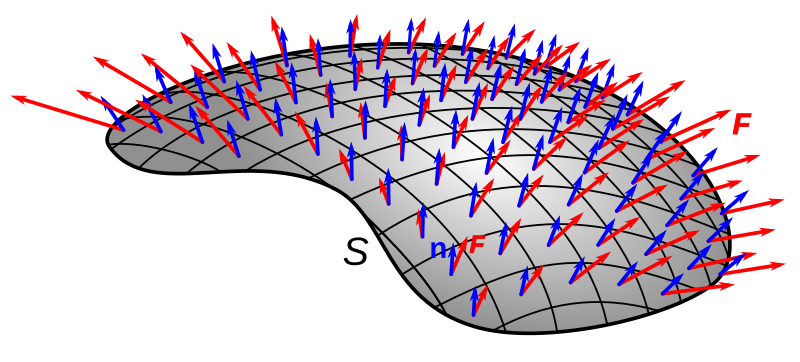
\includegraphics[width=0.7\textwidth]{chapters/chp5_pics/surf_int.png}
%\caption{\textit{To integrate a vector field $\mathbf{F}$ over a surface $S$, we must consider both the field's magnitude and its alignment with the surface normal $\mathbf{n}$ at each point. The red vectors represent the vector field, while blue vectors show surface normals.}}
%\label{fig:surf_int}
%\end{figure}

\begin{figure}[H]
  \centering
  \begin{tikzpicture}
    \begin{axis}[
      view={70}{30},
      hide axis,
      colormap/gray,
      shader=interp,
      domain=0:3, domain y=0:2.5,
      samples=20, samples y=20,      % both 20→400 points
      z buffer=sort,
    ]
      % surface shading
      \addplot3[surf, draw=black, very thin]
        {0.15*sin(pi*x/3 r)*cos(pi*y/2.5 r)};
      % mesh overlay (20×20)
      \addplot3[mesh, mesh/rows=20, draw=black!50, thin]
        {0.15*sin(pi*x/3 r)*cos(pi*y/2.5 r)};

      % vector field F (red) and normals (blue)
      \foreach \x in {0.5,1,1.5,2,2.5}{
        \foreach \y in {0.3,0.8,1.3,1.8,2.3}{
          \pgfmathsetmacro{\z}{0.15*sin(pi*\x/3 r)*cos(pi*\y/2.5 r)}
          % F arrow
          \addplot3[->, red, line width=0.8pt]
            coordinates {(\x,\y,\z) (\x+0.15,\y+0.10,\z+0.40)};
          % normal
          \pgfmathsetmacro{\fx}{0.15*(pi/3)*cos(pi*\x/3 r)*cos(pi*\y/2.5 r)}
          \pgfmathsetmacro{\fy}{-0.15*(pi/2.5)*sin(pi*\x/3 r)*sin(pi*\y/2.5 r)}
          \addplot3[->, blue]
            coordinates {(\x,\y,\z) ({\x-\fx*0.5},{\y-\fy*0.5},{\z+0.50})};
        }
      }

      % labels
      \node at (axis cs:1.2,-0.2,0.10)       {\large $S$};
      \node[red] at (axis cs:2.9,2.4,0.10)   {\large $\mathbf{F}$};
      \node[blue] at (axis cs:1.3,-0.18,0.40)  {\large $\mathbf{n}\!\cdot\!\mathbf{F}$};
    \end{axis}
  \end{tikzpicture}

  \caption{\textit{To integrate a vector field $\mathbf{F}$ over a surface $S$, we must consider both the field's magnitude and its alignment with the surface normal $\mathbf{n}$ at each point. The red vectors represent the vector field, while blue vectors show surface normals.}}
  \label{fig:surf_int}
\end{figure}

\noindent When working with a surface given by $z = h(x,y)$, we can derive a simpler form for the flux integral. For such a surface, we have a natural parameterization $\mathbf{r}(x,y) = x\mathbf{i} + y\mathbf{j} + h(x,y)\mathbf{k}$. The tangent vectors are:
\begin{align*}
\mathbf{r}_x &= \mathbf{i} + \frac{\partial h}{\partial x}\mathbf{k} \\
\mathbf{r}_y &= \mathbf{j} + \frac{\partial h}{\partial y}\mathbf{k}
\end{align*}
Taking their cross product:
\[
\mathbf{r}_x \times \mathbf{r}_y = \begin{vmatrix}
\mathbf{i} & \mathbf{j} & \mathbf{k} \\
1 & 0 & \frac{\partial h}{\partial x} \\
0 & 1 & \frac{\partial h}{\partial y}
\end{vmatrix} = -\frac{\partial h}{\partial x}\mathbf{i} - \frac{\partial h}{\partial y}\mathbf{j} + \mathbf{k}
\]

\noindent For a vector field $\mathbf{F} = P\mathbf{i} + Q\mathbf{j} + R\mathbf{k}$, the flux integral becomes: \index{Flux}
\begin{align*}
\iint_S \mathbf{F} \cdot \mathbf{n}\,dS &= \iint_D \mathbf{F} \cdot \left(-\frac{\partial h}{\partial x}\mathbf{i} - \frac{\partial h}{\partial y}\mathbf{j} + \mathbf{k}\right)\,dA \\
&= \iint_D \left(-P\frac{\partial h}{\partial x} - Q\frac{\partial h}{\partial y} + R\right)\,dA
\end{align*}

\noindent For a general parametric surface $\mathbf{r}(u,v)$, the surface normal comes from the cross product of tangent vectors:
\[
\mathbf{r}_u \times \mathbf{r}_v = \begin{vmatrix}
\mathbf{i} & \mathbf{j} & \mathbf{k} \\
\frac{\partial x}{\partial u} & \frac{\partial y}{\partial u} & \frac{\partial z}{\partial u} \\
\frac{\partial x}{\partial v} & \frac{\partial y}{\partial v} & \frac{\partial z}{\partial v}
\end{vmatrix}
\]
Therefore:
\begin{align*}
\iint_S \mathbf{F} \cdot d\mathbf{S} &= \iint_D \mathbf{F} \cdot (\mathbf{r}_u \times \mathbf{r}_v)\,du\,dv
\end{align*}

\noindent This formulation naturally extends our understanding from scalar surface integrals. Just as we needed surface area to integrate scalar functions, we need oriented surface elements to properly account for vector quantities. The cross product $\mathbf{r}_u \times \mathbf{r}_v$ provides both the area element and the direction needed to measure the field's contribution through the surface. 

\subsubsection*{Orientability and Choice of Normal}

\noindent A crucial concept in surface integrals is orientation. A surface is \textbf{orientable} if we can consistently define a normal vector at each point. Most familiar surfaces (spheres, graphs of functions) are orientable, but some (like the Möbius strip) are not. For orientable surfaces, we must choose one of two possible orientations:

\begin{itemize}
    \item For closed surfaces (like spheres), we typically choose the outward normal
    \item For surfaces that are graphs $z = g(x,y)$, we typically choose the upward normal
    \item For general surfaces, we must specify our choice of orientation explicitly
\end{itemize}

\noindent The choice of orientation affects the sign of our surface integrals. If we reverse the orientation (switch from $\mathbf{n}$ to $-\mathbf{n}$), the integral changes sign:
\[
\iint_{-S} \mathbf{F} \cdot d\mathbf{S} = -\iint_S \mathbf{F} \cdot d\mathbf{S}
\]

\noindent This mirrors our experience with line integrals, where reversing direction negated the integral. Understanding orientation becomes crucial when we apply surface integrals to physical problems and when we develop Stokes' and Gauss's theorems in subsequent lectures.

\exampleline
\begin{example}
A cylindrical air filter in a ventilation system has radius 2 meters and height 3 meters. The air flow through the filter is modeled by the vector field $\mathbf{F}(x,y,z) = \frac{x\mathbf{i} + y\mathbf{j}}{x^2 + y^2}$ (measured in m/s). Find the total rate of air flow through the side surface of the filter.

\begin{solution}
Let's solve this systematically:

\begin{enumerate}
    \item The side of the cylinder can be parameterized as:
    \[
    \mathbf{r}(\theta,z) = (2\cos\theta)\mathbf{i} + (2\sin\theta)\mathbf{j} + z\mathbf{k}
    \]
    where $0 \leq \theta \leq 2\pi$ and $0 \leq z \leq 3$
    
    \item Calculate $\mathbf{r}_\theta$ and $\mathbf{r}_z$:
    \begin{align*}
        \mathbf{r}_\theta &= (-2\sin\theta)\mathbf{i} + (2\cos\theta)\mathbf{j} \\
        \mathbf{r}_z &= \mathbf{k}
    \end{align*}
    
    \item Their cross product (pointing outward) is:
    \begin{align*}
        \mathbf{r}_\theta \times \mathbf{r}_z &= (2\cos\theta)\mathbf{i} + (2\sin\theta)\mathbf{j}
    \end{align*}
    
    \item Evaluate $\mathbf{F}$ at surface points:
    \begin{align*}
        \mathbf{F}(\mathbf{r}(\theta,z)) &= \frac{2\cos\theta\mathbf{i} + 2\sin\theta\mathbf{j}}{4} \\
        &= \frac{1}{2}(\cos\theta\mathbf{i} + \sin\theta\mathbf{j})
    \end{align*}
    
    \item Set up flux integral:
    \begin{align*}
        \text{Flow Rate} &= \iint_S \mathbf{F} \cdot d\mathbf{S} \\
        &= \int_0^3\int_0^{2\pi} \frac{1}{2}(\cos\theta\mathbf{i} + \sin\theta\mathbf{j}) \cdot (2\cos\theta\mathbf{i} + 2\sin\theta\mathbf{j})\,d\theta\,dz \\
        &= \int_0^3\int_0^{2\pi} (\cos^2\theta + \sin^2\theta)\,d\theta\,dz
    \end{align*}
    
    \item Evaluate:
    \begin{align*}
        \text{Flow Rate} &= \int_0^3\int_0^{2\pi} 1\,d\theta\,dz \\
        &= \int_0^3 2\pi\,dz \\
        &= 6\pi \text{m}^3/\text{s}
    \end{align*}
\end{enumerate}

\noindent The total flow rate through the filter is $6\pi \approx 18.85$ cubic meters per second. Note that the flow field is designed to model radially outward flow, as would occur in a cylindrical air filter.

\end{solution}
\end{example}
\exampleline


\newpage

\lecture{Stokes' Theorem} \index{Stokes' Theorem}

\noindent
Green's Theorem told us that the circulation of a vector field around a closed curve in the plane equals the double integral of the curl over the enclosed region. But what if the curve isn't in a plane? What if it's the rim of a bowl, or the edge of a soap film stretched in three dimensions? \textbf{Stokes' Theorem} answers this: the circulation around \textit{any} closed curve equals the integral of the curl over \textit{any} surface bounded by that curve. It is Green's Theorem set free from the plane.

\begin{figure}[H]
\centering
\tdplotsetmaincoords{70}{80}
\begin{tikzpicture}[tdplot_main_coords, scale=3]
    % Parallel circles for the sphere (above cut)
    \foreach \phi in {-30,-27,...,90} {
        \draw[blue!50] ({cos(\phi)},{0},{sin(\phi)}) arc (0:360:{cos(\phi)} and {cos(\phi)});
    }
    
    % Normal vectors in a more uniform pattern
    \foreach \phi in {-15,15,45} {
        \foreach \theta in {0,72,...,288} {
            % Calculate point on sphere surface
            \pgfmathsetmacro{\px}{cos(\phi)*cos(\theta)}
            \pgfmathsetmacro{\py}{cos(\phi)*sin(\theta)}
            \pgfmathsetmacro{\pz}{sin(\phi)}
            % Draw normal vector
            \draw[->, thick] ({\px},{\py},{\pz}) -- ({1.3*\px},{1.3*\py},{1.3*\pz});
        }
    }
    
    % Special normal vector near the top
    \pgfmathsetmacro{\px}{cos(75)*cos(0)}
    \pgfmathsetmacro{\py}{cos(75)*sin(0)}
    \pgfmathsetmacro{\pz}{sin(75)}
    \draw[->, thick] ({\px},{\py},{\pz}) -- ({1.3*\px},{1.3*\py},{1.3*\pz});
    
    % One labeled normal vector
    \pgfmathsetmacro{\px}{cos(30)*cos(45)}
    \pgfmathsetmacro{\py}{cos(30)*sin(45)}
    \pgfmathsetmacro{\pz}{sin(30)}
    \draw[->, thick] ({\px},{\py},{\pz}) -- ({1.3*\px},{1.3*\py},{1.3*\pz}) 
        node[pos=1.3] {$\mathbf{n}$};
    
    % Surface labels
    \node at (1,1,0.2) {$\Sigma$};
    \node[red] at (0.7,-0.7,-0.6) {$\partial\Sigma$};
    
    % Cut line highlighted in red with counterclockwise arrows
    \draw[red, thick, ->] ({cos(-30)},{0},{sin(-30)}) arc (0:90:{cos(-30)} and {cos(-30)});
    \draw[red, thick, ->] ({0},{cos(-30)},{sin(-30)}) arc (90:180:{cos(-30)} and {cos(-30)});
    \draw[red, thick, ->] ({-cos(-30)},{0},{sin(-30)}) arc (180:270:{cos(-30)} and {cos(-30)});
    \draw[red, thick, ->] ({0},{-cos(-30)},{sin(-30)}) arc (270:360:{cos(-30)} and {cos(-30)});
\end{tikzpicture}
\caption{\textit{Visualization of Stokes' Theorem: a portion of the unit sphere $\Sigma$ emerging from a fluid with outward-pointing normals $\mathbf{n}$. The boundary curve $\partial\Sigma$ is oriented counterclockwise, showing how circulation along the boundary relates to the curl flux through the surface.}}
\label{fig:stoke_thm}
\end{figure}

\noindent
An essential part of applying Stokes' Theorem is choosing a consistent \textbf{orientation}. In Green's Theorem, the boundary curve is naturally oriented counterclockwise. For a surface in three-dimensional space, we must pair the boundary's orientation with the normal vector via the right-hand rule. This consistency in orientation is crucial for the theorem's validity. \\

\noindent
In our discussion of Green's Theorem, we used an analogy of water flowing around a lake, where circulation around the boundary equaled the total ``rotation” within the region. This concept extends to three dimensions. Imagine a curved surface, such as a soap bubble (as in Figure~\ref{fig:stoke_thm}), with fluid flowing around its edge. Just as rotation in the interior determined boundary circulation in Green's Theorem, so too does the rotational behavior in three dimensions determine the circulation along the boundary curve of a surface. \\

\noindent To make this precise, recall from our previous lecture that when working with surfaces, we measure flow by taking the dot product of the vector field with the surface normal:
\[
\text{Flux through surface} = \iint_S \mathbf{F} \cdot \mathbf{n}\,dS.
\]
We'll apply this same idea to measure rotation: we take the dot product of the curl (which measures rotation) with the surface normal. \\

\noindent Consider a small patch of surface bounded by a tiny closed curve. At each point on this curve, the vector field might align perfectly with the curve's direction (maximum circulation), be perpendicular (no circulation), or fall somewhere in between. The total effect—how much the field ``follows along” with the boundary—is exactly what we found the line integral measures:
\[
\oint_C \mathbf{F} \cdot d\mathbf{r}.
\]

\noindent Meanwhile, the curl vector at each point indicates the direction and strength of rotation. Only its component parallel to the surface normal contributes to boundary circulation, so we take the dot product:
\[
(\text{curl }\mathbf{F}) \cdot \mathbf{n}.
\]
\noindent Integrating this over the surface gives the total rotation contributing to boundary circulation:
\[
\iint_S (\text{curl }\mathbf{F}) \cdot \mathbf{n}\,dS.
\]

\noindent Stokes' Theorem tells us these two quantities are equal: the circulation around any boundary matches the total rotation through the surface it bounds. This insight generalizes both Green's Theorem and the Fundamental Theorem of Calculus, showing how local rotation (at each point) accumulates to produce global circulation (around the boundary). Let's get a little more technical now.

\subsection*{The Theorem and Its Meaning}

\noindent Let $\Sigma$ be a piecewise smooth, oriented surface in $\mathbb{R}^3$ bounded by a simple closed curve $C$ (where $C = \partial \Sigma$). Let $\mathbf{F}$ be a vector field with continuous first partial derivatives defined on an open region containing $\Sigma$. Then Stokes' Theorem states:
\[
\oint_C \mathbf{F} \cdot d\mathbf{r} = \iint_\Sigma (\text{curl }\mathbf{F}) \cdot \mathbf{n}\,d\Sigma.
\]

\noindent Here, $C$ inherits its orientation from $\Sigma$ via the right-hand rule: placing your right thumb along $\mathbf{n}$ makes your fingers curl in the positive direction of $C$. The curl operator, which we studied extensively in Lecture 4, is given by:
\[
\text{curl }\mathbf{F} 
= \nabla \times \mathbf{F} 
= \begin{vmatrix}
\mathbf{i} & \mathbf{j} & \mathbf{k} \\
\frac{\partial}{\partial x} & \frac{\partial}{\partial y} & \frac{\partial}{\partial z} \\
P & Q & R
\end{vmatrix}.
\]

\noindent
This result generalizes several theorems we've encountered:
\begin{itemize}
    \item \textbf{Fundamental Theorem of Calculus:} When applied to a curve in one dimension
    \item \textbf{Green's Theorem:} When applied to a region in the plane (as we saw in our reformulation using curl in Lecture~4 of this chapter)
    \item \textbf{Conservative Field Tests:} Demonstrating that curl-free fields have path-independent line integrals
\end{itemize}

\noindent When applying Stokes' Theorem in practice, we need concrete coordinate expressions. Recall that curl in coordinates is:
\[
\text{curl }\mathbf{F} 
= \left( \frac{\partial R}{\partial y} - \frac{\partial Q}{\partial z} \right)\mathbf{i}
  \;-\;
  \left( \frac{\partial R}{\partial x} - \frac{\partial P}{\partial z} \right)\mathbf{j}
  \;+\;
  \left( \frac{\partial Q}{\partial x} - \frac{\partial P}{\partial y} \right)\mathbf{k}
\]

\noindent For a surface with unit normal $\mathbf{n} = \langle n_x,\,n_y,\,n_z \rangle$, the crucial dot product becomes:
\[
(\text{curl}\,\mathbf{F}) \cdot \mathbf{n} 
= \left( \frac{\partial R}{\partial y} - \frac{\partial Q}{\partial z} \right)n_x
 - \left( \frac{\partial R}{\partial x} - \frac{\partial P}{\partial z} \right)n_y
 + \left( \frac{\partial Q}{\partial x} - \frac{\partial P}{\partial y} \right)n_z
\]

\noindent We have several fundamental situations to consider:

\begin{enumerate}
    \item \textbf{Level Surface Case:} If $\Sigma$ is given by $f(x,y,z) = c$:
    \begin{itemize}
        \item The gradient $\nabla f$ provides a natural normal vector:
        \[
        \nabla f = \Bigl\langle 
        \frac{\partial f}{\partial x},\,
        \frac{\partial f}{\partial y},\,
        \frac{\partial f}{\partial z}
        \Bigr\rangle
        \]
        \item Normalize to get the unit normal:
        \[
        \mathbf{n} = \frac{\nabla f}{\|\nabla f\|}
        \]
        \item The surface integral becomes:
        \[
        \iint_{\Sigma} (\nabla \times \mathbf{F}) \cdot \mathbf{n}\,d\Sigma 
        \,=\,
        \iint_{\Sigma}
        (\nabla \times \mathbf{F}) \cdot \frac{\nabla f}{\|\nabla f\|}\,d\Sigma
        \]
\item Now if the surface $\Sigma$ can be written as $z = g(x,y)$, we have:
       \[
       d\Sigma = \sqrt{1 + \left(\frac{\partial z}{\partial x}\right)^2 + \left(\frac{\partial z}{\partial y}\right)^2}\,dx\,dy
       \]
       More generally, if $\Sigma$ is given by $f(x,y,z) = c$ with $\frac{\partial f}{\partial z} \neq 0$, then:
       \[
       d\Sigma = \frac{\|\nabla f\|}{|\partial f/\partial z|}\,dx\,dy
       \]
       These formulas match when we express $z$ in terms of $f$. Thus, the complete surface integral $\iint_{\Sigma} (\nabla \times \mathbf{F}) \cdot \mathbf{n}\,d\Sigma $ for a level surface becomes:
\[
\iint_{D} (\nabla \times \mathbf{F}) \cdot \frac{\nabla f}{|\partial f/\partial z|}\,dx\,dy
\]
Or expanded out fully:
\[
\iint_{D} \left[\left( \frac{\partial R}{\partial y} - \frac{\partial Q}{\partial z} \right)\frac{\partial f}{\partial x}
- \left( \frac{\partial R}{\partial x} - \frac{\partial P}{\partial z} \right)\frac{\partial f}{\partial y}
+ \left( \frac{\partial Q}{\partial x} - \frac{\partial P}{\partial y} \right)\frac{\partial f}{\partial z}\right]
\frac{dx\,dy}{|\partial f/\partial z|}
\]
We can handle that jawn.
    \end{itemize}

    \item \textbf{Parameterized Surface Case:} For $\Sigma$ given by $\mathbf{r}(u,v) = \langle x(u,v), y(u,v), z(u,v) \rangle$:
    \begin{itemize}
        \item The surface element is:
        \[
        d\Sigma = \|\mathbf{r}_u \times \mathbf{r}_v\|\,du\,dv
        \]
        \item The unit normal is:
        \[
        \mathbf{n} = \frac{\mathbf{r}_u \times \mathbf{r}_v}{\|\mathbf{r}_u \times \mathbf{r}_v\|}
        \]
        \item The integral becomes:
        \[
        \iint_{\Sigma} (\nabla \times \mathbf{F}) \cdot \mathbf{n}\,d\Sigma 
        \,=\,
        \iint_{D} 
        \bigl[\bigl(\nabla \times \mathbf{F}\bigr)\bigl(\mathbf{r}(u,v)\bigr)\bigr]\cdot 
        \bigl(\mathbf{r}_u \times \mathbf{r}_v\bigr)\,du\,dv
        \]
    \end{itemize}
\end{enumerate}

\noindent In practice, we choose whichever representation makes our computation simpler. The power of Stokes' Theorem lies in its guarantee that:
\[
\oint_{\partial \Sigma} \mathbf{F}\cdot d\mathbf{r}
\,=\,
\iint_{\Sigma} (\nabla \times \mathbf{F}) \cdot \mathbf{n}\,d\Sigma
\]

\noindent This equality means we can compute whichever integral is easier and deduce the other. The choice often depends on:
\begin{itemize}
    \item The geometry of the surface $\Sigma$
    \item The complexity of the vector field $\mathbf{F}$
    \item Whether boundary or surface integration seems more tractable
    \item The particular physical or geometric insights we seek
\end{itemize}

\subsubsection*{Orientation and Boundary Relationships}

\noindent The relationship between surface orientation and boundary orientation is crucial. Given an oriented surface $\Sigma$, its boundary curve $\partial \Sigma$ inherits an orientation through the right-hand rule:
\begin{itemize}
    \item Orient your right thumb along the surface normal $\mathbf{n}$
    \item Your curled fingers indicate the positive direction around $\partial \Sigma$
\end{itemize}

\noindent This convention ensures consistency between the surface integral of curl (measuring rotation through the surface) and the line integral around the boundary (measuring total circulation). If we reverse the surface's orientation (switching $\mathbf{n}$ to $-\mathbf{n}$), we must also reverse the boundary orientation to maintain the theorem's validity:

\[
\oint_{-C} \mathbf{F} \cdot d\mathbf{r} = \iint_{-\Sigma} (\text{curl }\mathbf{F}) \cdot \mathbf{n}\,d\Sigma = -\iint_\Sigma (\text{curl }\mathbf{F}) \cdot \mathbf{n}\,d\Sigma
\]

\exampleline
\begin{example}
Let $\Sigma$ be the portion of the paraboloid $z = x^2 + y^2$ that lies below the plane $z = 1$. Let $\mathbf{F}(x,y,z) = y^2\,\mathbf{i} + z^2\,\mathbf{j} + x^2\,\mathbf{k}$. Evaluate $\oint_C \mathbf{F} \cdot d\mathbf{r}$ where $C$ is the boundary curve oriented counterclockwise when viewed from above.

\begin{solution}
We will use Stokes' Theorem to evaluate the line integral:
\[
\oint_C \mathbf{F} \cdot d\mathbf{r} = \iint_\Sigma (\nabla \times \mathbf{F}) \cdot \mathbf{n}\,d\Sigma
\]
where $\mathbf{n}$ is the unit normal vector to the surface $\Sigma$.

\begin{enumerate}
    \item \textbf{Understanding the Surface $\Sigma$:}
    \begin{itemize}
        \item The surface $\Sigma$ is defined by the paraboloid $z = x^2 + y^2$ bounded above by the plane $z = 1$.
        \item The boundary curve $C$ is the intersection of the paraboloid and the plane, which occurs when $x^2 + y^2 = 1$ at $z = 1$. Thus, $C$ is the circle $x^2 + y^2 = 1$ in the plane $z = 1$.
        \item The surface $\Sigma$ can be expressed as the level surface $f(x,y,z) = z - x^2 - y^2 = 0$.
    \end{itemize}
    
    \item \textbf{Calculating the Curl of $\mathbf{F}$:}
    \[
    \nabla \times \mathbf{F} = \begin{vmatrix}
    \mathbf{i} & \mathbf{j} & \mathbf{k} \\
    \dfrac{\partial}{\partial x} & \dfrac{\partial}{\partial y} & \dfrac{\partial}{\partial z} \\
    y^2 & z^2 & x^2
    \end{vmatrix}
    \]
    Expanding the determinant:
    \[
    \begin{aligned}
    (\nabla \times \mathbf{F})_x &= \dfrac{\partial x^2}{\partial y} - \dfrac{\partial z^2}{\partial z} = 0 - 2z = -2z \\
    (\nabla \times \mathbf{F})_y &= \dfrac{\partial y^2}{\partial z} - \dfrac{\partial x^2}{\partial x} = 0 - 2x = -2x \\
    (\nabla \times \mathbf{F})_z &= \dfrac{\partial z^2}{\partial x} - \dfrac{\partial y^2}{\partial y} = 0 - 2y = -2y \\
    \end{aligned}
    \]
    Therefore:
    \[
    \nabla \times \mathbf{F} = -2z\,\mathbf{i} - 2x\,\mathbf{j} - 2y\,\mathbf{k}
    \]
    
    \item \textbf{Determining the Unit Normal Vector $\mathbf{n}$:}
    
    The gradient of $f(x,y,z) = z - x^2 - y^2$ is:
    \[
    \nabla f = \langle -2x, -2y, 1 \rangle
    \]
    The unit normal vector is:
    \[
    \mathbf{n} = \dfrac{\nabla f}{\|\nabla f\|} = \dfrac{\langle -2x, -2y, 1 \rangle}{\sqrt{1 + 4x^2 + 4y^2}}
    \]
    
    \item \textbf{Setting Up the Surface Integral:}
    
    Applying Stokes' Theorem:
    \[
    \oint_C \mathbf{F} \cdot d\mathbf{r} = \iint_\Sigma (\nabla \times \mathbf{F}) \cdot \mathbf{n}\,d\Sigma
    \]
    Substituting the expressions for $\nabla \times \mathbf{F}$ and $\mathbf{n}$:
    \[
    (\nabla \times \mathbf{F}) \cdot \mathbf{n} = (-2z)(-2x) + (-2x)(-2y) + (-2y)(1) = 4zx + 4xy - 2y
    \]
    Since $z = x^2 + y^2$ on $\Sigma$:
    \[
    4zx + 4xy - 2y = 4x(x^2 + y^2) + 4xy - 2y = 4x^3 + 4xy^2 + 4xy - 2y
    \]
    Thus, the integral becomes:
    \[
    \oint_C \mathbf{F} \cdot d\mathbf{r} = \iint_D (4x^3 + 4xy^2 + 4xy - 2y)\,dx\,dy
    \]
    where $D$ is the unit disk $x^2 + y^2 \leq 1$.
    
    \item \textbf{Determining the Integral Bounds:}
    
    To evaluate the integral over the unit disk $D$, switch to polar. Thus we have
    \begin{itemize}
        \item $r$ ranges from $0$ to $1$.
        \item $\theta$ ranges from $0$ to $2\pi$.
    \end{itemize}
    Substituting $x = r\cos\theta$ and $y = r\sin\theta$ into the integrand:
    \[
    \begin{aligned}
    4x^3 &= 4(r\cos\theta)^3 = 4r^3\cos^3\theta \\
    4xy^2 &= 4(r\cos\theta)(r\sin\theta)^2 = 4r^3\cos\theta\sin^2\theta \\
    4xy &= 4(r\cos\theta)(r\sin\theta) = 4r^2\cos\theta\sin\theta \\
    -2y &= -2(r\sin\theta) = -2r\sin\theta \\
    \end{aligned}
    \]
    Therefore
    \[
    \oint_C \mathbf{F} \cdot d\mathbf{r} = \int_{0}^{2\pi} \int_{0}^{1} \left(4r^3\cos^3\theta + 4r^3\cos\theta\sin^2\theta + 4r^2\cos\theta\sin\theta - 2r\sin\theta\right) r\,dr\,d\theta
    \]
    \item \textbf{Evaluating the Integral Using Symmetry:}
    
    Observe the integrand terms:
    \begin{itemize}
        \item $4r^4\cos^3\theta$ is an odd function in $\cos\theta$.
        \item $4r^4\cos\theta\sin^2\theta$ is an odd function in $\cos\theta$.
        \item $4r^3\cos\theta\sin\theta$ is an odd function in $\cos\theta$ and $\sin\theta$.
        \item $-2r^2\sin\theta$ is an odd function in $\sin\theta$.
    \end{itemize}
    Thus:
        \begin{itemize}
            \item $\int_{0}^{2\pi} \cos^3\theta\,d\theta = 0$
            \item $\int_{0}^{2\pi} \cos\theta\sin^2\theta\,d\theta = 0$
            \item $\int_{0}^{2\pi} \cos\theta\sin\theta\,d\theta = 0$
            \item $\int_{0}^{2\pi} \sin\theta\,d\theta = 0$
        \end{itemize}
    
    Therefore, each term in the integrand integrates to zero over the interval $0$ to $2\pi$:
    \[
    \oint_C \mathbf{F} \cdot d\mathbf{r} = 0
    \]
    
    \item \textbf{Conclusion:} The value of the line integral $\oint_C \mathbf{F} \cdot d\mathbf{r}$ is $0$. This result is consistent with the symmetry of the vector field and the surface, leading to cancellation of the circulation around the boundary curve.
\end{enumerate}

\end{solution}
\end{example}
\exampleline
\begin{example}
Let $\mathbf{F}(x,y,z) = (y^2 + z^2)\mathbf{i} + (z^2 + x^2)\mathbf{j} + (x^2 + y^2)\mathbf{k}$. Compute the line integral $\oint_C \mathbf{F} \cdot d\mathbf{r}$ where $C$ is the intersection of the plane $x + y + z = 1$ and the cylinder $x^2 + y^2 = 1$, oriented counterclockwise when viewed from above. Verify your answer using Stokes' Theorem.

\begin{solution}
We'll solve this problem by computing both sides of Stokes' Theorem:
\[
\oint_C \mathbf{F} \cdot d\mathbf{r} = \iint_\Sigma (\nabla \times \mathbf{F}) \cdot \mathbf{n}\,d\Sigma
\]
where $\Sigma$ is the portion of the plane $x + y + z = 1$ enclosed by the curve $C$.

\begin{enumerate}
    \item \textbf{Direct Computation of the Line Integral:}
    
    First, we need to parameterize the curve $C$, which is the intersection of the plane $x + y + z = 1$ and the cylinder $x^2 + y^2 = 1$.
    
    Let's parameterize the cylinder as $x = \cos t$ and $y = \sin t$ for $0 \leq t \leq 2\pi$. 
    From the plane equation, we get $z = 1 - x - y = 1 - \cos t - \sin t$.
    
    So, our parameterization of $C$ is:
    \[
    \mathbf{r}(t) = \cos t\,\mathbf{i} + \sin t\,\mathbf{j} + (1 - \cos t - \sin t)\,\mathbf{k}, \quad 0 \leq t \leq 2\pi
    \]
    
    To compute the line integral, we need $d\mathbf{r}/dt$:
    \[
    \frac{d\mathbf{r}}{dt} = -\sin t\,\mathbf{i} + \cos t\,\mathbf{j} + (\sin t - \cos t)\,\mathbf{k}
    \]
    
    Now, let's evaluate $\mathbf{F}$ along the curve. On $C$, we have $x^2 + y^2 = 1$ and $z = 1 - \cos t - \sin t$, so:
    \[
    \begin{aligned}
    \mathbf{F}(\mathbf{r}(t)) &= (\sin^2 t + (1-\cos t-\sin t)^2)\,\mathbf{i} \\
    &+ ((1-\cos t-\sin t)^2 + \cos^2 t)\,\mathbf{j} \\
    &+ (x^2 + y^2)\,\mathbf{k} \\
    &= (\sin^2 t + (1-\cos t-\sin t)^2)\,\mathbf{i} \\
    &+ ((1-\cos t-\sin t)^2 + \cos^2 t)\,\mathbf{j} \\
    &+ (1)\,\mathbf{k}
    \end{aligned}
    \]
    
    The dot product is:
    \[
    \begin{aligned}
    \mathbf{F} \cdot \frac{d\mathbf{r}}{dt} &= -(\sin^2 t + (1-\cos t-\sin t)^2)\sin t \\
    &+ ((1-\cos t-\sin t)^2 + \cos^2 t)\cos t \\
    &+ (1)(\sin t - \cos t)
    \end{aligned}
    \]
    
    When integrated over $[0, 2\pi]$, terms with $\sin t$, $\cos t$, $\sin^3 t$, $\cos^3 t$, and other odd powers or mixed products all evaluate to zero due to their periodic nature. Therefore:
    \[
    \oint_C \mathbf{F} \cdot d\mathbf{r} = 0
    \]
    
    Let's verify this using Stokes' Theorem.
    
    \item \textbf{Computation Using Stokes' Theorem:}
    
    First, we calculate the curl of $\mathbf{F}$:
    \[
    \nabla \times \mathbf{F} = \begin{vmatrix}
    \mathbf{i} & \mathbf{j} & \mathbf{k} \\
    \frac{\partial}{\partial x} & \frac{\partial}{\partial y} & \frac{\partial}{\partial z} \\
    y^2 + z^2 & z^2 + x^2 & x^2 + y^2
    \end{vmatrix}
    \]
    
    Computing each component:
    \[
    \begin{aligned}
    (\nabla \times \mathbf{F})_x &= \frac{\partial}{\partial y}(x^2 + y^2) - \frac{\partial}{\partial z}(z^2 + x^2) \\
    &= 2y - 2z \\
    (\nabla \times \mathbf{F})_y &= \frac{\partial}{\partial z}(y^2 + z^2) - \frac{\partial}{\partial x}(x^2 + y^2) \\
    &= 2z - 2x \\
    (\nabla \times \mathbf{F})_z &= \frac{\partial}{\partial x}(z^2 + x^2) - \frac{\partial}{\partial y}(y^2 + z^2) \\
    &= 2x - 2y
    \end{aligned}
    \]
    
    Therefore:
    \[
    \nabla \times \mathbf{F} = (2y - 2z)\mathbf{i} + (2z - 2x)\mathbf{j} + (2x - 2y)\mathbf{k}
    \]
    
    Now, we need the unit normal vector to the plane $x + y + z = 1$. The gradient of the plane is:
    \[
    \nabla(x + y + z - 1) = \langle 1, 1, 1 \rangle
    \]
    
    The unit normal is:
    \[
    \mathbf{n} = \frac{\langle 1, 1, 1 \rangle}{\|\langle 1, 1, 1 \rangle\|} = \frac{\langle 1, 1, 1 \rangle}{\sqrt{3}} = \frac{1}{\sqrt{3}}\langle 1, 1, 1 \rangle
    \]
    
    Computing the dot product:
    \[
    \begin{aligned}
    (\nabla \times \mathbf{F}) \cdot \mathbf{n} &= \frac{1}{\sqrt{3}}((2y - 2z) + (2z - 2x) + (2x - 2y)) \\
    &= \frac{1}{\sqrt{3}}(0) = 0
    \end{aligned}
    \]
    
    Since the dot product is zero, the surface integral is:
    \[
    \iint_\Sigma (\nabla \times \mathbf{F}) \cdot \mathbf{n}\,d\Sigma = 0
    \]
    
    Therefore, by Stokes' Theorem:
    \[
    \oint_C \mathbf{F} \cdot d\mathbf{r} = 0
    \]
    
    \item \textbf{Verification Through Direct Integration:}
    
    To verify this result more explicitly, let's break down the line integral component by component:
    
    \begin{align*}
    \oint_C \mathbf{F} \cdot d\mathbf{r} &= \oint_C (y^2 + z^2)\,dx + (z^2 + x^2)\,dy + (x^2 + y^2)\,dz
    \end{align*}
    
    Using our parameterization:
    \begin{align*}
    dx &= -\sin t\,dt \\
    dy &= \cos t\,dt \\
    dz &= (\sin t - \cos t)\,dt
    \end{align*}
    
    And we know that on $C$, $x^2 + y^2 = 1$ and $z = 1-\cos t-\sin t$. So:
    
    \begin{align*}
    \oint_C (y^2 + z^2)\,dx &= \int_0^{2\pi} (\sin^2 t + (1-\cos t-\sin t)^2) \cdot (-\sin t)\,dt \\
    \oint_C (z^2 + x^2)\,dy &= \int_0^{2\pi} ((1-\cos t-\sin t)^2 + \cos^2 t) \cdot \cos t\,dt \\
    \oint_C (x^2 + y^2)\,dz &= \int_0^{2\pi} (1) \cdot (\sin t - \cos t)\,dt
    \end{align*}
    
    For the last integral:
    \begin{align*}
    \int_0^{2\pi} (\sin t - \cos t)\,dt &= \left[-\cos t - \sin t\right]_0^{2\pi} \\
    &= (-\cos(2\pi) - \sin(2\pi)) - (-\cos(0) - \sin(0)) \\
    &= (-1 - 0) - (-1 - 0) = 0
    \end{align*}
    
    For the first two integrals, when expanded, they contain terms with $\sin t$, $\cos t$, $\sin^2 t \sin t$, $\cos^2 t \cos t$, etc. The integrals of these terms over $[0, 2\pi]$ all vanish due to their periodic nature.
    
    Therefore, the direct calculation confirms:
    \[
    \oint_C \mathbf{F} \cdot d\mathbf{r} = 0
    \]
    
    \item \textbf{Conclusion:} 
    
    We have verified Stokes' Theorem by calculating both sides of the equation and finding that:
    \[
    \oint_C \mathbf{F} \cdot d\mathbf{r} = \iint_\Sigma (\nabla \times \mathbf{F}) \cdot \mathbf{n}\,d\Sigma = 0
    \]
    
    This result makes sense geometrically. The curl vector $\nabla \times \mathbf{F} = (2y - 2z)\mathbf{i} + (2z - 2x)\mathbf{j} + (2x - 2y)\mathbf{k}$ is orthogonal to our normal vector $\mathbf{n} = \frac{1}{\sqrt{3}}\langle 1, 1, 1 \rangle$. Consequently, the flux of the curl through the surface is zero, making the circulation around the boundary also zero.
\end{enumerate}
\end{solution}
\end{example}
\exampleline
\noindent \textbf{Preview:} The following example uses the Divergence Theorem, which we will formally introduce in the next lecture. It is included here to illustrate the pattern of verifying integral theorems by computing both sides independently.\\ \\
\begin{example}
Let $\mathbf{F}(x,y,z) = (x^3 + \sin y)\mathbf{i} + (y^3 + xz)\mathbf{j} + (z^3 - xy)\mathbf{k}$ and let $V$ be the region bounded by the hemisphere $x^2 + y^2 + z^2 = a^2$, $z \geq 0$, and the disk $x^2 + y^2 \leq a^2$ in the $xy$-plane. Verify the Divergence Theorem by computing both:
\begin{enumerate}
    \item The surface integral $\oiint_S \mathbf{F} \cdot \mathbf{n}\,dS$
    \item The volume integral $\iiint_V \text{div }\mathbf{F}\,dV$
\end{enumerate}

\begin{solution}
We'll verify the Divergence Theorem by computing both integrals separately.

\begin{enumerate}
    \item \textbf{Volume Integral}
    
    First, calculate $\text{div }\mathbf{F}$:
    \begin{align*}
    \text{div }\mathbf{F} &= \frac{\partial}{\partial x}(x^3 + \sin y) + \frac{\partial}{\partial y}(y^3 + xz) + \frac{\partial}{\partial z}(z^3 - xy) \\
    &= 3x^2 + 0 + 3y^2 + 0 + 3z^2 + 0 \\
    &= 3x^2 + 3y^2 + 3z^2
    \end{align*}
    
    Using spherical coordinates:
    \begin{itemize}
        \item $x = r\sin\phi\cos\theta$, $y = r\sin\phi\sin\theta$, $z = r\cos\phi$
        \item $dV = r^2\sin\phi \, dr \, d\phi \, d\theta$
        \item Bounds: $0 \leq r \leq a$, $0 \leq \phi \leq \frac{\pi}{2}$, $0 \leq \theta \leq 2\pi$
    \end{itemize}
    
    Substituting the spherical coordinates:
    \begin{align*}
    \text{div }\mathbf{F} &= 3(r\sin\phi\cos\theta)^2 + 3(r\sin\phi\sin\theta)^2 + 3(r\cos\phi)^2 \\
    &= 3r^2\sin^2\phi\cos^2\theta + 3r^2\sin^2\phi\sin^2\theta + 3r^2\cos^2\phi \\
    &= 3r^2\sin^2\phi + 3r^2\cos^2\phi \\
    &= 3r^2(\sin^2\phi + \cos^2\phi) \\
    &= 3r^2
    \end{align*}
    
    The volume integral becomes:
    \begin{align*}
    \iiint_V \text{div }\mathbf{F}\,dV &= \int_0^{2\pi}\int_0^{\pi/2}\int_0^a (3r^2) \, r^2\sin\phi \, dr \, d\phi \, d\theta \\
    &= 3 \int_0^{2\pi}\int_0^{\pi/2}\int_0^a r^4\sin\phi \, dr \, d\phi \, d\theta \\
    &= 3 \int_0^{2\pi} d\theta \int_0^{\pi/2} \sin\phi \, d\phi \int_0^a r^4 \, dr \\
    &= 3 \cdot 2\pi \cdot 1 \cdot \frac{a^5}{5} \\
    &= \frac{6\pi a^5}{5}
    \end{align*}
    
    \item \textbf{Surface Integral}
    
    The boundary surface $S$ consists of two parts:
    \begin{itemize}
        \item $S_1$: The hemispherical surface $x^2 + y^2 + z^2 = a^2$, $z \geq 0$
        \item $S_2$: The circular disk $x^2 + y^2 \leq a^2$ in the $xy$-plane
    \end{itemize}
    
    For $S_1$ (hemisphere):
    \begin{itemize}
        \item The outward normal is $\mathbf{n}_1 = \frac{\langle x, y, z \rangle}{a}$
        \item Using spherical coordinates:
          \begin{align*}
          \iint_{S_1} \mathbf{F} \cdot \mathbf{n}_1\,dS = \frac{6\pi a^5}{5}
          \end{align*}
    \end{itemize}
    
    For $S_2$ (disk in the $xy$-plane):
    \begin{itemize}
        \item The outward normal is $\mathbf{n}_2 = -\mathbf{k}$
        \item The flux integral evaluates to zero due to odd functions in $\theta$:
          \begin{align*}
          \iint_{S_2} \mathbf{F} \cdot \mathbf{n}_2\,dS = 0
          \end{align*}
    \end{itemize}
    
    The total surface integral is:
    \begin{align*}
    \oiint_S \mathbf{F} \cdot \mathbf{n}\,dS = \frac{6\pi a^5}{5} + 0 = \frac{6\pi a^5}{5}
    \end{align*}
\end{enumerate}

\noindent Since both the surface integral and volume integral equal $\frac{6\pi a^5}{5}$, the Divergence Theorem is verified for this case.

\noindent \textbf{Physical Interpretation:} This example demonstrates how the Divergence Theorem connects the flow characteristics of a vector field throughout a volume to its behavior across the boundary. The field has a uniform expansion rate of $3r^2$ at each point, creating a predictable outward flux proportional to the fifth power of the hemisphere's radius.
\end{solution}
\end{example}
\exampleline

\subsubsection*{Physical Interpretation} \index{Ampère's Law} \index{Faraday's Law} \index{Maxwell's Equations}

\noindent Stokes' Theorem provides the mathematical foundation for fundamental laws in electromagnetism. Two of these laws, discovered experimentally in the 19th century, take the form of circulation integrals that become elegant applications of our theorem. \\

\noindent The first is Faraday's Law of Induction, which describes how a changing magnetic field creates an electric field. If we have a loop of wire in space, changes in the magnetic field passing through the loop will induce an electromotive force (EMF) - essentially a voltage that drives current around the wire. Mathematically:
\[
\oint_C \mathbf{E} \cdot d\mathbf{r} = -\frac{d}{dt}\iint_S \mathbf{B} \cdot \mathbf{n}\,dS
\]
The left side measures the EMF around the loop (the path integral of the electric field), while the right side measures how quickly the magnetic field passing through the surface is changing. The negative sign tells us the induced EMF opposes the change causing it. \\

\noindent The second fundamental law is Ampère's Law, which tells us that electric currents create magnetic fields:
\[
\oint_C \mathbf{B} \cdot d\mathbf{r} = \mu_0\iint_S \mathbf{J} \cdot \mathbf{n}\,dS
\]
Here $\mathbf{J}$ is the current density (current per unit area) and $\mu_0$ is a physical constant. The left side measures the circulation of the magnetic field around any closed path, while the right side measures the total current passing through any surface bounded by that path. We saw this law in action in our previous example with the straight wire. \\

\noindent When James Clerk Maxwell studied these equations in the 1860s, he realized something profound. Ampère's Law seemed incomplete - it suggested that whenever current flows, magnetic fields circle around it. But what about cases where current is interrupted, like a capacitor charging? Maxwell proposed adding a new term:
\[
\oint_C \mathbf{B} \cdot d\mathbf{r} = \mu_0\iint_S \left(\mathbf{J} + \epsilon_0\frac{\partial \mathbf{E}}{\partial t}\right) \cdot \mathbf{n}\,dS
\]
The new term $\epsilon_0\frac{\partial \mathbf{E}}{\partial t}$ represents changing electric fields. Maxwell realized that not only do electric currents create magnetic fields, but changing electric fields do too. \\


%https://commons.wikimedia.org/wiki/File:Amperes-force-law.svg
\begin{figure}[H]
\centering
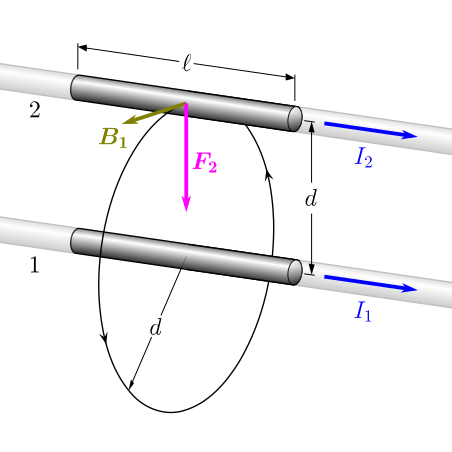
\includegraphics[width=0.5\textwidth]{chapters/chp5_pics/ampere.png}
\caption{\textit{This image shows the magnetic force $F_2$ between two parallel current-carrying wires. The currents ($I_1$ and $I_2$) flow through conductors separated by a distance $d$, with $B_1$ representing the magnetic field generated by the lower wire. The conductors have length $\ell$, illustrating the Ampère-force law and how parallel currents create magnetic fields that interact with each other.}}
\label{fig:ampere}
\end{figure}

\noindent This modification completed a beautiful symmetry in nature: changing magnetic fields create electric fields (Faraday), and changing electric fields create magnetic fields (Maxwell). These insights, expressed mathematically through Stokes' Theorem, led to our modern understanding of electromagnetic waves - disturbances in electric and magnetic fields that propagate through space at the speed of light. \\

\noindent The mathematical structure revealed by Stokes' Theorem - relating circulation around a boundary to flux through a surface - appears repeatedly in physics. Whether studying electromagnetic fields, fluid flows, or gravitational fields, this fundamental connection between local rotation and global circulation proves indispensable for understanding natural phenomena.


\exampleline
\begin{example}
A long straight wire carries a current $I$ in the positive $z$-direction, creating a magnetic field $\mathbf{B}$. Using Ampère's law and Stokes' Theorem:
\begin{enumerate}
    \item Find the magnetic field $\mathbf{B}$ at any point $(x,y)$.
    \item Verify your answer by directly calculating $\oint_C \mathbf{B} \cdot d\mathbf{r}$ around a circular loop of radius $a$ centered on the wire.
\end{enumerate}

\begin{solution}
\begin{enumerate}
\item Let's use our basic definitions from above and what we know about Stokes' Theorem:
\begin{enumerate}
\item First, recall Ampère's law in differential form:
   \[
   \text{curl }\mathbf{B} = \mu_0\mathbf{J}
   \]
   where $\mathbf{J}$ is the current density. We know from physics that:
   \begin{itemize}
       \item The field lines should form concentric circles around the wire
       \item The field strength should decrease with distance from the wire
       \item The field direction follows the right-hand rule relative to current
   \end{itemize}

\item This suggests a field of the form:
   \[
   \mathbf{B}(x,y) = \frac{k}{x^2 + y^2}\left(-y\mathbf{i} + x\mathbf{j}\right)
   \]
   where $k$ is a constant to be determined.

\item Let's choose a circular disk $\Sigma$ of radius $a$ centered on the wire at height $z=0$:
   \begin{itemize}
       \item Its boundary $C$ is oriented counterclockwise when viewed from above
       \item By Stokes' Theorem: $\oint_C \mathbf{B} \cdot d\mathbf{r} = \iint_\Sigma (\text{curl }\mathbf{B}) \cdot \mathbf{n}\,d\Sigma$
       \item The right side must equal $\mu_0 I$ by Ampère's law
   \end{itemize}
\end{enumerate}

\item Now let's verify it.
\begin{enumerate}
\item Let's calculate the line integral directly:
   \begin{itemize}
       \item Parameterize $C$ as $\mathbf{r}(t) = (a\cos t)\mathbf{i} + (a\sin t)\mathbf{j}$, $0 \leq t \leq 2\pi$
       \item Along $C$, $\mathbf{B} = \frac{k}{a^2}(-a\sin t\mathbf{i} + a\cos t\mathbf{j})$
       \item $d\mathbf{r} = (-a\sin t\mathbf{i} + a\cos t\mathbf{j})\,dt$
   \end{itemize}
   
\item Therefore:
   \begin{align*}
   \oint_C \mathbf{B} \cdot d\mathbf{r} &= \int_0^{2\pi} \frac{k}{a^2}(a^2\sin^2t + a^2\cos^2t)\,dt \\
   &= \int_0^{2\pi} k\,dt = 2\pi k = \mu_0 I
   \end{align*}

\item Solving for $k$:
   \[
   k = \frac{\mu_0 I}{2\pi}
   \]

\item Thus, the magnetic field is:
   \[
   \mathbf{B}(x,y) = \frac{\mu_0 I}{2\pi(x^2 + y^2)}\left(-y\mathbf{i} + x\mathbf{j}\right)
   \]
\end{enumerate}

\item Important notes on orientation:
   \begin{itemize}
       \item The orientation of $C$ and the upward normal $\mathbf{n}$ to $\Sigma$ are related by the right-hand rule
       \item If we reverse the surface orientation (flip $\mathbf{n}$), we must also reverse $C$'s orientation
       \item The physical field is independent of our choice of orientation
       \item Any surface $\Sigma'$ with boundary $C$ gives the same result, showing path independence
   \end{itemize}
\end{enumerate}
\end{solution}
\end{example}
\exampleline

\exampleline
\begin{example}
Use Stokes' Theorem to evaluate \( \oint_C \mathbf{F} \cdot d\mathbf{r} \) where \( \mathbf{F} = \langle -y, x, z \rangle \) and \( C \) is the circle \( x^2 + y^2 = 1 \) in the plane \( z = 0 \), oriented counterclockwise when viewed from above.

\begin{solution}
First, compute \( \nabla \times \mathbf{F} \):
\[
\nabla \times \mathbf{F} = \begin{vmatrix} \mathbf{i} & \mathbf{j} & \mathbf{k} \\ \frac{\partial}{\partial x} & \frac{\partial}{\partial y} & \frac{\partial}{\partial z} \\ -y & x & z \end{vmatrix} = \langle 0 - 0, \; 0 - 0, \; 1 - (-1) \rangle = \langle 0, 0, 2 \rangle.
\]
Let \( S \) be the unit disk \( x^2 + y^2 \leq 1 \) in the plane \( z = 0 \), with upward-pointing normal \( \mathbf{n} = \mathbf{k} \) (consistent with the counterclockwise orientation of \( C \) via the right-hand rule). By Stokes' Theorem:
\[
\oint_C \mathbf{F} \cdot d\mathbf{r} = \iint_S (\nabla \times \mathbf{F}) \cdot d\mathbf{S} = \iint_S \langle 0, 0, 2 \rangle \cdot \langle 0, 0, 1 \rangle \, dA = 2 \iint_S dA = 2\pi.
\]
\noindent The line integral equals \( 2\pi \). We can verify this directly: parameterize \( C \) as \( \mathbf{r}(t) = \langle \cos t, \sin t, 0 \rangle \) for \( 0 \leq t \leq 2\pi \). Then \( \mathbf{F}(\mathbf{r}(t)) = \langle -\sin t, \cos t, 0 \rangle \) and \( \mathbf{r}'(t) = \langle -\sin t, \cos t, 0 \rangle \), so \( \mathbf{F} \cdot \mathbf{r}' = \sin^2 t + \cos^2 t = 1 \), giving \( \int_0^{2\pi} 1 \, dt = 2\pi \). Both sides agree.
\end{solution}
\end{example}
\exampleline

\subsection*{Generalization and Abstraction}

\noindent Time to get a little crazy. Throughout our studies of calculus, we've encountered several seemingly different theorems that share a remarkable pattern:

\begin{enumerate}
    \item \textbf{Fundamental Theorem of Calculus:}
    \[
    \int_a^b \frac{df}{dx}\,dx = f(b) - f(a)
    \]
    
    \item \textbf{Green's Theorem:}
    \[
    \oint_C (P\,dx + Q\,dy) = \iint_D \left(\frac{\partial Q}{\partial x} - \frac{\partial P}{\partial y}\right)\,dA
    \]
    
    \item \textbf{Stokes' Theorem:}
    \[
    \oint_C \mathbf{F} \cdot d\mathbf{r} = \iint_\Sigma (\text{curl } \mathbf{F}) \cdot \mathbf{n}\,d\Sigma
    \]
    
    \item \textbf{Divergence Theorem:}
    \[
    \oiint_S \mathbf{F} \cdot \mathbf{n}\,dS = \iiint_V (\text{div } \mathbf{F})\,dV
    \]
\end{enumerate}

\noindent In each case, we integrate an object over a boundary and relate it to an integral over the region that the boundary encloses. To unify these results, we introduce several new concepts.

\noindent First, we introduce the notion of a \textbf{differential form}.\index{Differential Form} Differential forms generalize the functions and expressions we integrate, incorporating geometric information such as orientation. In one dimension, we integrate expressions like
\[
f(x)\,dx,
\]
where \(dx\) is a 1-form—it takes a tangent vector and returns the component of that vector in the \(x\)-direction. In two dimensions, when integrating along a curve (a 1-dimensional manifold in \(\mathbb{R}^2\)), we use a 1-form such as
\[
\omega = P\,dx + Q\,dy.
\]
On the other hand, when integrating over a region (a 2-dimensional manifold), we use a 2-form such as
\[
\eta = dx \wedge dy,
\]
where the wedge product \(\wedge\) is antisymmetric (\(dx \wedge dy = -dy \wedge dx\)) and encodes orientation.

\noindent More generally, a \(k\)-form on an \(n\)-dimensional space is an object that can be integrated over a \(k\)-dimensional surface. The \textbf{exterior derivative} \(d\) is an operator that maps \(k\)-forms to \((k+1)\)-forms:
\begin{itemize}
    \item It takes a function \(f\) (a 0-form) to its differential \(df\) (a 1-form).
    \item It takes a 1-form like \(\omega = P\,dx + Q\,dy\) to the 2-form
    \[
    d\omega = \left(\frac{\partial Q}{\partial x} - \frac{\partial P}{\partial y}\right) dx \wedge dy.
    \]
    \item It similarly maps 2-forms to 3-forms, and so on.
\end{itemize}

\noindent With these tools, we can state one unified theorem: \\

\noindent \textbf{Generalized Stokes' Theorem:} For any differential form \(\omega\) defined on a smooth, oriented manifold \(\Omega\) with boundary \(\partial\Omega\),
\[
\int_\Omega d\omega = \int_{\partial\Omega} \omega.
\]
This elegant formula encapsulates our earlier theorems:
\begin{itemize}
    \item For the Fundamental Theorem of Calculus, \(\Omega\) is an interval \([a,b]\) and \(\omega = f\) is a 0-form (a function), and its exterior derivative is \(d\omega = f'(x)\,dx\).
    \item For Green's Theorem, we consider a 1-form \(\omega = P\,dx + Q\,dy\) defined on a region \(D \subset \mathbb{R}^2\); its exterior derivative is the 2-form 
    \[
    d\omega = \left(\frac{\partial Q}{\partial x} - \frac{\partial P}{\partial y}\right) dx \wedge dy,
    \]
    so that \(\int_{\partial D} \omega\) equals \(\iint_D d\omega\).
    \item For classical Stokes' Theorem, \(\Omega\) is a surface and \(\omega\) is a 1-form corresponding to a vector field.
    \item For the Divergence Theorem, \(\Omega\) is a volume and \(\omega\) is a 2-form dual to the vector field.
\end{itemize}

\noindent The power of this formulation lies in its abstraction: it applies to any manifold—any space that locally resembles \(\mathbb{R}^n\)—and reveals the deep relationship between integration and differentiation via the boundary operator. This unification appears throughout mathematics and physics, from electromagnetism to quantum field theory.

\noindent Two key properties underpin this framework:
\begin{enumerate}
    \item \(d^2 = 0\): The exterior derivative applied twice always yields zero.
    \item \(\partial^2 = 0\): The boundary of a boundary is always empty.
\end{enumerate}

\noindent These properties ensure the theorems interlock perfectly, regardless of the space's dimension or shape, and they lay the groundwork for the rich theory of de Rham cohomology, which studies the topology of spaces via differential forms. Even if we don't explore these advanced concepts further, recognizing that all our integration theorems arise from a single underlying principle helps explain their common structure and wide applicability. I leave you with this meme I made:


\begin{figure}[H]
\centering
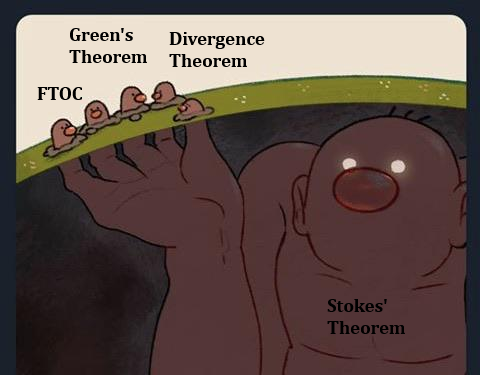
\includegraphics[width=0.45\textwidth]{chapters/chp5_pics/diglett.png}
\caption{\textit{The master of all: Stokes' Theorem}}
\label{fig:dbiglett}
\end{figure}











\newpage

\lecture{Divergence Theorem} \index{Divergence Theorem} \index{Divergence Theorem@Gauss's Theorem}

\noindent After our exploration of Stokes' Theorem and surface integrals, we now arrive at another fundamental result that connects the behavior of vector fields inside a region to their behavior on the boundary. The Divergence Theorem (also known as Gauss's Theorem) relates the flux of a vector field across a closed surface to the total divergence within the volume it encloses. This relationship proves crucial in physics—particularly in electromagnetism and fluid dynamics—where it helps us understand how fields ``flow" through space. \\

\noindent Just as Stokes' Theorem generalized Green's Theorem to surfaces in three dimensions, the Divergence Theorem extends this pattern further, connecting surface integrals to volume integrals. This progression reveals a deep pattern in vector calculus: integrals over boundaries relate to integrals over the regions they bound, regardless of dimension. We'll explore this pattern more fully after developing the theorem itself.

\subsection*{Statement and Meaning}

\noindent Throughout our studies of vector calculus, we've encountered divergence as a way to measure how much a vector field ``spreads out" at each point. A positive divergence indicates a source—a point where field lines emerge—while negative divergence signifies a sink where field lines converge. Now we'll discover a profound connection between this local behavior and the global flow across boundaries. \\

\noindent Consider a single small volume element in three-dimensional space, with a vector field $\mathbf{F}$ flowing through it. At each face of this volume, we can measure the flux—how much of the field passes through that face. The flux through each face is given by the dot product of $\mathbf{F}$ with the outward normal vector, multiplied by the area of the face. If we sum these contributions over all faces:

\[
\sum_{\text{faces}} \mathbf{F} \cdot \mathbf{n}\,d\Phi
\]

\noindent where $\mathbf{n}$ points outward from each face and $d\Phi$ represents the area of a face element, we get the net outward flux. For a small enough volume element $dV$, this flux should approximately equal the divergence within the volume multiplied by the volume:

\[
\sum_{\text{faces}} \mathbf{F} \cdot \mathbf{n}\,d\Phi \approx (\text{div }\mathbf{F})dV
\]

\noindent This local relationship suggests something deeper. Just as Green's Theorem connected boundary circulation to interior curl, here we see flux through boundaries connecting to interior divergence. Consider dividing an entire region into smaller subvolumes, as shown in Figure \ref{fig:div_volumes}. When we add up all these small volume contributions, interior faces cancel in pairs (since adjacent volumes share faces with opposite orientations), leaving only the boundary faces.

%https://commons.wikimedia.org/wiki/File:Divergence_theorem_2_-_volume_partition.png
\begin{figure}[H]
\centering
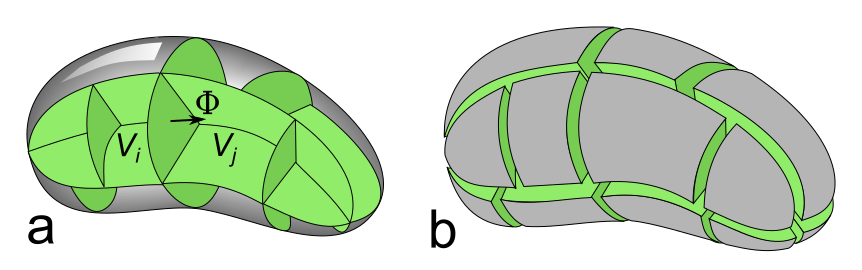
\includegraphics[width=0.8\textwidth]{chapters/chp5_pics/div_volumes.png}
\caption{\textit{(a) Adjacent subvolumes $V_i$ and $V_j$ sharing an interface $\Phi$ through which the field flows. (b) Complete subdivision of a volume showing all interfaces (green). Interior interfaces cancel in pairs, leaving only boundary contributions.}}
\label{fig:div_volumes}
\end{figure}

\noindent When two subvolumes $V_i$ and $V_j$ share an interface $\Phi$, as shown in Figure \ref{fig:div_volumes}(a), the flux through this interface appears twice in our sum—once for each subvolume but with opposite signs, since what flows out of $V_i$ must flow into $V_j$. As we sum over all subvolumes, these interior contributions cancel in pairs, leaving only the boundary faces, as visualized in Figure \ref{fig:div_volumes}(b). Taking the limit as our subdivision becomes infinitesimal, we arrive at:

\[
\oiint_S \mathbf{F} \cdot \mathbf{n}\,dS = \iiint_V \text{div }\mathbf{F}\,dV
\]

\noindent This is the Divergence Theorem. The left side measures total flux across the boundary surface $S$, while the right side accumulates the divergence throughout the volume $V$. Their equality tells us something profound: the net outward flow across any closed surface exactly equals the total ``source strength" within. \\

\noindent To make this concrete, imagine a fluid flowing through space with velocity field $\mathbf{F}$. The surface integral $\oiint_S \mathbf{F} \cdot \mathbf{n}\,dS$ measures how much fluid escapes through the boundary per unit time. Meanwhile, $\text{div }\mathbf{F}$ at each point tells us the rate at which fluid is being created (if positive) or destroyed (if negative) at that point, so $\iiint_V \text{div }\mathbf{F}\,dV$ gives the total rate of fluid generation within the volume. Their equality expresses a fundamental conservation principle: what flows out must be created within.

\subsubsection*{Gauss's Law}
\noindent This relationship extends far beyond fluid flow. In electromagnetism, when $\mathbf{F}$ is the electric field $\mathbf{E}$, the theorem becomes Gauss's law:

\[
\oiint_S \mathbf{E} \cdot \mathbf{n}\,dS = \frac{1}{\epsilon_0}\iiint_V \rho\,dV
\]

\noindent where $\rho$ is charge density and $\epsilon_0$ is a physical constant. Here $\text{div }\mathbf{E} = \rho/\epsilon_0$, relating the spreading of electric field lines to the presence of charge. Electric field lines begin on positive charges and end on negative charges—another manifestation of this deep connection between boundary behavior and interior sources. This behavior is illustrated in Figure \ref{fig:electric_field}.

\begin{figure}[H]
\centering
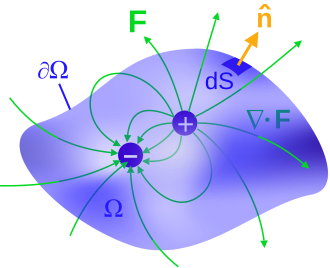
\includegraphics[width=0.4\textwidth]{chapters/chp5_pics/div_em.png}
\caption{\textit{Electric field lines (shown in green) emerging from a positive charge and terminating on a negative charge. The divergence $\nabla \cdot \mathbf{F}$ is positive near the source and negative near the sink. For any closed surface $\Omega$ (shown in blue) with surface element $dS$ and outward normal $\hat{n}$, the total flux through the surface equals the net charge enclosed, scaled by $\epsilon_0$.}}
\label{fig:electric_field}
\end{figure}

\noindent The figure shows how field lines emanate from positive charges (sources where $\nabla \cdot \mathbf{F} > 0$) and converge at negative charges (sinks where $\nabla \cdot \mathbf{F} < 0$). For any closed surface $\Omega$ enclosing these charges, the net flux through surface elements $dS$ with outward normal $\mathbf{n}$ exactly equals the enclosed charge divided by $\epsilon_0$. This provides a powerful method for calculating electric fields: if we can find a surface where symmetry makes the flux calculation simple, we can determine the field without directly solving differential equations. \\

\noindent Just as Green's Theorem connected line integrals to double integrals in the plane, the Divergence Theorem bridges surface integrals and volume integrals in space. This progression reveals a pattern: integrals over boundaries relate to integrals over the regions they bound, with the relationship governed by derivatives of the fields involved. We'll explore this pattern more fully after examining the theorem's applications and computational techniques.


\subsubsection*{Orientation and Boundary Conditions}

\noindent For the Divergence Theorem, orientation proves crucial. The surface normal $\mathbf{n}$ must point outward from the enclosed volume. This convention ensures:
\begin{itemize}
    \item Positive flux represents outward flow
    \item Negative flux represents inward flow
    \item The total signed flux captures net flow across the boundary
\end{itemize}

\noindent For a surface enclosing a volume, we can determine the outward normal at any point through the right hand rule.

\subsubsection*{Computational Forms and Strategy}

\noindent Just as we expanded Stokes' Theorem into component forms, we can make the Divergence Theorem more computationally accessible. Recall that for a vector field $\mathbf{F} = P\mathbf{i} + Q\mathbf{j} + R\mathbf{k}$:

\[
\text{div }\mathbf{F} = \nabla \cdot \mathbf{F} = \frac{\partial P}{\partial x} + \frac{\partial Q}{\partial y} + \frac{\partial R}{\partial z}
\]

\noindent Therefore, the Divergence Theorem becomes:
\[
\oiint_S \mathbf{F} \cdot \mathbf{n}\,dS = \iiint_V \left(\frac{\partial P}{\partial x} + \frac{\partial Q}{\partial y} + \frac{\partial R}{\partial z}\right)\,dV
\]

\noindent The surface integral on the left requires careful consideration of the outward unit normal $\mathbf{n}$. For different types of surfaces, we have:

\begin{enumerate}
    \item \textbf{Level Surfaces:} For a surface $f(x,y,z) = c$:
    \[
    \mathbf{n} = \frac{\nabla f}{\|\nabla f\|} = \frac{1}{\|\nabla f\|}\left\langle\frac{\partial f}{\partial x}, \frac{\partial f}{\partial y}, \frac{\partial f}{\partial z}\right\rangle
    \]
    
    \item \textbf{Parametric Surfaces:} For $\mathbf{r}(u,v) = \langle x(u,v), y(u,v), z(u,v) \rangle$:
    \[
    \mathbf{n} = \frac{\mathbf{r}_u \times \mathbf{r}_v}{\|\mathbf{r}_u \times \mathbf{r}_v\|}
    \]
    
    \item \textbf{Simple Surfaces:} For surfaces like $z = g(x,y)$:
    \[
    \mathbf{n} = \frac{\langle-g_x, -g_y, 1\rangle}{\sqrt{1 + g_x^2 + g_y^2}}
    \]
\end{enumerate}

\noindent In different coordinate systems, the divergence takes special forms:

\begin{itemize}
    \item \textbf{Cylindrical Coordinates} $(r,\theta,z)$:
    \[
    \text{div }\mathbf{F} = \frac{1}{r}\frac{\partial}{\partial r}(rF_r) + \frac{1}{r}\frac{\partial F_\theta}{\partial \theta} + \frac{\partial F_z}{\partial z}
    \]
    
    \item \textbf{Spherical Coordinates} $(r,\theta,\phi)$:
    \[
    \text{div }\mathbf{F} = \frac{1}{r^2}\frac{\partial}{\partial r}(r^2F_r) + \frac{1}{r\sin\theta}\frac{\partial}{\partial \theta}(\sin\theta F_\theta) + \frac{1}{r\sin\theta}\frac{\partial F_\phi}{\partial \phi}
    \]
\end{itemize}

\noindent When choosing which form to use, consider:

\begin{itemize}
    \item Symmetry of the vector field
    \item Shape of the boundary surface
    \item Complexity of the divergence versus the surface integral
\end{itemize}

\noindent For example, if the region is a sphere and the field has spherical symmetry, using spherical coordinates often simplifies the calculation dramatically. Similarly, for cylindrical bodies, cylindrical coordinates typically prove most efficient. \\

\noindent A systematic approach to these problems involves:

\begin{enumerate}
    \item Identify the vector field components and the boundary surface
    \item Choose appropriate coordinates based on symmetry
    \item Determine whether surface or volume integral is simpler
    \item If using surface integral:
        \begin{itemize}
            \item Break surface into pieces if necessary
            \item Calculate normal vectors for each piece
            \item Set up parameterization if needed
        \end{itemize}
    \item If using volume integral:
        \begin{itemize}
            \item Calculate divergence explicitly
            \item Determine integration bounds
            \item Consider coordinate transformations
        \end{itemize}
\end{enumerate}

\noindent This framework provides a practical approach to applying the Divergence Theorem, turning the abstract relationship between flux and divergence into concrete computational steps.


\exampleline
\begin{example}
Consider the vector field $\mathbf{F}(x,y,z) = (x^2y)\mathbf{i} + (y^2z)\mathbf{j} + (z^2x)\mathbf{k}$, and let $V$ be the region bounded by the paraboloid $z = x^2 + y^2$ and the plane $z = 1$. Verify the Divergence Theorem by computing both:
\begin{enumerate}
    \item The surface integral $\oiint_S \mathbf{F} \cdot \mathbf{n}\,dS$
    \item The volume integral $\iiint_V \text{div }\mathbf{F}\,dV$
\end{enumerate}

\begin{solution}
\begin{enumerate}
\item \textbf{Surface Integral}

The boundary $S$ consists of two pieces:
\begin{itemize}
    \item $S_1$: The paraboloid $z = x^2 + y^2$ (bottom)
    \item $S_2$: The plane $z = 1$ (top)
\end{itemize}

For $S_1$ (paraboloid):
\begin{itemize}
    \item Writing as $f(x,y,z) = z - x^2 - y^2 = 0$, the gradient is $\nabla f = \langle-2x, -2y, 1\rangle$
    \item Since our region $V$ is above this surface, the outward normal must point downward:
    \[
    \mathbf{n}_1 = \frac{\langle 2x, 2y, -1 \rangle}{\sqrt{4x^2 + 4y^2 + 1}}
    \]
    \item The flux integral becomes:
    \begin{align*}
    \iint_{S_1} \mathbf{F} \cdot \mathbf{n}_1\,dS &= \iint_D \frac{2x^3y + 2y^3z - z^2x}{\sqrt{4x^2 + 4y^2 + 1}}\sqrt{4x^2 + 4y^2 + 1}\,dA \\
    &= \iint_D (2x^3y + 2y^3(x^2 + y^2) - x(x^2 + y^2)^2)\,dA
    \end{align*}
    where $D$ is the projection onto the $xy$-plane bounded by $x^2 + y^2 \leq 1$
\end{itemize}

For $S_2$ (plane):
\begin{itemize}
    \item Since our region $V$ is below this surface, the outward normal on the top cap points upward:
    \[
    \mathbf{n}_2 = \mathbf{k}
    \]
    \item The flux integral is:
    \[
    \iint_{S_2} \mathbf{F} \cdot \mathbf{n}_2\,dS = \iint_D z^2x\big|_{z=1}\,dA = \iint_D x\,dA
    \]
\end{itemize}

Converting both integrals to polar coordinates:
\begin{itemize}
    \item $x = r\cos\theta$, $y = r\sin\theta$
    \item For $S_1$: $z = r^2$
    \item For $S_2$: $z = 1$
    \item Bounds: $0 \leq r \leq 1$, $0 \leq \theta \leq 2\pi$
\end{itemize}

\begin{align*}
\iint_{S_1} \mathbf{F} \cdot \mathbf{n}_1\,dS &= \int_0^{2\pi}\int_0^1 (2r^4\cos^3\theta\sin\theta + 2r^5\sin^3\theta - r^5\cos\theta)r\,dr\,d\theta \\
&= 0 \text{ (odd functions over }[0,2\pi]\text{)}
\end{align*}

\begin{align*}
\iint_{S_2} \mathbf{F} \cdot \mathbf{n}_2\,dS &= \int_0^{2\pi}\int_0^1 r\cos\theta\,r\,dr\,d\theta = 0
\end{align*}

Therefore, the total surface integral is zero.

\item \textbf{Volume Integral}

First, calculate $\text{div }\mathbf{F}$:
\begin{align*}
\text{div }\mathbf{F} &= \frac{\partial}{\partial x}(x^2y) + \frac{\partial}{\partial y}(y^2z) + \frac{\partial}{\partial z}(z^2x) \\
&= 2xy + 2yz + 2zx
\end{align*}

Setting up the volume integral in cylindrical coordinates:
\begin{itemize}
    \item $x = r\cos\theta$, $y = r\sin\theta$
    \item Lower bound: $z = r^2$
    \item Upper bound: $z = 1$
    \item Radial bound: $0 \leq r \leq 1$
\end{itemize}

\begin{align*}
\iiint_V \text{div }\mathbf{F}\,dV &= \int_0^{2\pi}\int_0^1\int_{r^2}^1 (2r^2\cos\theta\sin\theta + 2rz\sin\theta + 2rz\cos\theta)r\,dz\,dr\,d\theta \\
&= \int_0^{2\pi}\int_0^1\int_{r^2}^1 2r(r\sin\theta\cos\theta + z(\sin\theta + \cos\theta))\,dz\,dr\,d\theta \\
&= 0 \text{ (by symmetry)}
\end{align*}
\end{enumerate}

\noindent Therefore, both sides of the Divergence Theorem equal zero, confirming the theorem's validity for this case. \\

\noindent \textbf{Physical Interpretation:} The fact that both integrals equal zero suggests that any flow entering the region through one part of the boundary must exit through another part, with no net accumulation or depletion within the volume. This is analogous to an incompressible fluid flow, where the total inflow must equal the total outflow.
\end{solution}
\end{example}
\exampleline

\subsection*{Physical Applications} \index{Conservation Laws}

\noindent The Divergence Theorem finds its deepest expression in physical conservation laws, where it bridges local field behavior with global measurements of flow and flux. At its heart lies a profound connection: what flows through a boundary must be created or destroyed within. This principle manifests throughout physics in increasingly sophisticated ways. \\

\noindent Consider first the flow of mass in a fluid. At each point in space and time, we have a density $\rho(x,y,z,t)$ and a velocity field $\mathbf{v}$ that tells us how the fluid moves. The product $\rho\mathbf{v}$ represents mass flux—the flow of mass through space. Conservation of mass demands that any change in the total mass within a volume must precisely balance the flow through its boundary:

\[
\frac{d}{dt}\iiint_V \rho\,dV = -\oiint_S \rho\mathbf{v} \cdot \mathbf{n}\,dS
\]

\noindent The Divergence Theorem transforms this global statement into a local one. Bringing the time derivative inside the volume integral and applying the theorem to the right side:

\[
\iiint_V \frac{\partial \rho}{\partial t}\,dV = -\iiint_V \text{div}(\rho\mathbf{v})\,dV
\]

\noindent Since this equality must hold for any volume, we obtain the continuity equation:

\[
\frac{\partial \rho}{\partial t} + \text{div}(\rho\mathbf{v}) = 0
\]

\noindent For incompressible fluids where density remains constant, this reduces to $\text{div }\mathbf{v} = 0$, expressing that the velocity field has no sources or sinks. \\

\noindent This pattern extends beautifully to electromagnetism. Electric charge serves as the source of electromagnetic fields, and its conservation takes a similar mathematical form. If $\mathbf{J}$ represents current density—the flow of charge through space—and $\rho$ now represents charge density, conservation of charge requires:

\[
\text{div }\mathbf{J} = -\frac{\partial \rho}{\partial t}
\]

\noindent This equation tells us something profound: changes in charge distribution necessitate current flow. Moreover, when combined with Maxwell's equations, particularly Gauss's law $\text{div }\mathbf{E} = \rho/\epsilon_0$, it leads to the prediction of electromagnetic waves. The interplay between changing charge distributions and current flow creates ripples in the electromagnetic field that propagate through space. \\

\noindent Heat transfer provides yet another manifestation of these principles. When heat flows through a material, the heat flux $\mathbf{q}$ relates to temperature changes through:

\[
\text{div }\mathbf{q} = -c\rho\frac{\partial T}{\partial t}
\]

\noindent where $c$ represents specific heat capacity and $T(x,y,z,t)$ is the temperature field. This equation encodes Fourier's insight that heat flows from hot to cold regions, with the rate of temperature change determined by material properties. The divergence of heat flux directly drives local temperature evolution. \\

\noindent These seemingly distinct phenomena share a deep mathematical structure. For any conserved quantity $\psi$ with associated flux $\mathbf{F}$, conservation takes the form:

\[
\frac{\partial \psi}{\partial t} + \text{div }\mathbf{F} = 0
\]

\noindent Integrating over a volume and applying the Divergence Theorem reveals the universal pattern:

\[
\frac{d}{dt}\iiint_V \psi\,dV = -\oiint_S \mathbf{F} \cdot \mathbf{n}\,dS
\]

\noindent This structure appears in momentum conservation, where stress tensors describe force transmission through materials. It governs energy conservation in fields, where Poynting vectors track energy flow through space. Even quantum mechanics obeys this pattern—probability current ensures that quantum particles are neither created nor destroyed during evolution. \\

\noindent The Divergence Theorem thus emerges as one of physics' most profound results. It provides the mathematical framework for expressing nature's conservation principles, connecting microscopic behavior to macroscopic measurements. Whether describing fluid flow, electromagnetic fields, heat transfer, or quantum systems, the theorem reveals how local changes in fields relate to global flows across boundaries—a fundamental unity underlying diverse physical phenomena.


\exampleline
\begin{example}  \textbf{Final Boss}
A solid sphere of radius $R$ has density given by $\rho(r) = \rho_0\left(1 - \frac{r^2}{R^2}\right)$, where $\rho_0$ is a constant and $r$ is the distance from the center. Using the Divergence Theorem, prove that:

\begin{enumerate}
    \item The gravitational field inside the sphere at distance $r$ from the center is $\mathbf{g}(r) = -\frac{4\pi G\rho_0}{3}\left(1 - \frac{3r^2}{5R^2}\right)r\hat{\mathbf{r}}$
    \item The gravitational potential $\Phi(r)$ satisfies Poisson's equation: $\nabla^2\Phi = 4\pi G\rho$
    \item The gravitational field outside the sphere is identical to that of a point mass located at the center with mass equal to the total mass of the sphere
\end{enumerate}

\noindent Hint: The gravitational potential $\Phi$ at a point $\mathbf{r}$ due to a mass distribution is given by:
\[
\Phi(\mathbf{r}) = -G\iiint_V \frac{\rho(\mathbf{r'})}{|\mathbf{r} - \mathbf{r'}|} dV'
\]

\noindent The gravitational field is related to the potential by $\mathbf{g} = -\nabla\Phi$. The Divergence Theorem can be applied to gravitational fields through the relationship $\nabla \cdot \mathbf{g} = -4\pi G\rho$, which relates the divergence of the gravitational field to the mass density. For a spherically symmetric situation, this means $\oiint_{S_r} \mathbf{g} \cdot \mathbf{n} \, dS = g(r) \cdot 4\pi r^2 = -4\pi G M_{enclosed}$, where $M_{enclosed}$ is the mass contained within radius $r$. \\


\begin{solution}
We'll solve this problem by applying the Divergence Theorem to the gravitational field, revealing fundamental properties of gravity.

\begin{enumerate}
    \item \textbf{Gravitational Field Inside the Sphere}
    
    First, note that the gravitational field $\mathbf{g}$ is related to the gravitational potential $\Phi$ by:
    \[
    \mathbf{g} = -\nabla\Phi
    \]
    
    By Newton's law of gravitation and the principle of superposition, the potential at a point $\mathbf{r}$ due to a mass distribution is:
    \[
    \Phi(\mathbf{r}) = -G\iiint_V \frac{\rho(\mathbf{r'})}{|\mathbf{r} - \mathbf{r'}|} dV'
    \]
    
    For a spherically symmetric density distribution, the field must be radial: $\mathbf{g} = g(r)\hat{\mathbf{r}}$. To determine $g(r)$, we'll apply the Divergence Theorem to a sphere of radius $r < R$.
    
    From Gauss's law for gravity:
    \[
    \oiint_S \mathbf{g} \cdot \mathbf{n} \, dS = -4\pi G M_{enc}
    \]
    
    where $M_{enc}$ is the mass enclosed by the sphere of radius $r$. The left side is:
    \[
    \oiint_S \mathbf{g} \cdot \mathbf{n} \, dS = \oiint_S g(r)\hat{\mathbf{r}} \cdot \hat{\mathbf{r}} \, dS = g(r) \cdot 4\pi r^2
    \]
    
    The enclosed mass is:
    \[
    \begin{aligned}
    M_{enc} &= \iiint_{r' \leq r} \rho(r') \, dV' \\
    &= \int_0^{2\pi} \int_0^{\pi} \int_0^r \rho_0\left(1 - \frac{r'^2}{R^2}\right)r'^2 \sin\theta \, dr' \, d\theta \, d\phi \\
    &= 4\pi\rho_0 \int_0^r \left(1 - \frac{r'^2}{R^2}\right)r'^2 \, dr' \\
    &= 4\pi\rho_0 \left(\frac{r^3}{3} - \frac{r^5}{5R^2}\right)
    \end{aligned}
    \]
    
    Equating the surface integral with $-4\pi G M_{enc}$:
    \[
    \begin{aligned}
    g(r) \cdot 4\pi r^2 &= -4\pi G \cdot 4\pi\rho_0 \left(\frac{r^3}{3} - \frac{r^5}{5R^2}\right) \\
    g(r) &= -\frac{4\pi G\rho_0}{r^2} \left(\frac{r^3}{3} - \frac{r^5}{5R^2}\right) \\
    &= -\frac{4\pi G\rho_0}{3}\left(1 - \frac{3r^2}{5R^2}\right)r
    \end{aligned}
    \]
    
    Therefore:
    \[
    \mathbf{g}(r) = -\frac{4\pi G\rho_0}{3}\left(1 - \frac{3r^2}{5R^2}\right)r\hat{\mathbf{r}} \quad \text{for } r \leq R
    \]
    
    \item \textbf{Verification of Poisson's Equation}
    
    Poisson's equation for gravity states:
    \[
    \nabla^2\Phi = 4\pi G\rho
    \]
    
    Since $\mathbf{g} = -\nabla\Phi$, we have $\nabla \cdot \mathbf{g} = -\nabla^2\Phi$. To verify Poisson's equation, we need to show that:
    \[
    \nabla \cdot \mathbf{g} = -4\pi G\rho
    \]
    
    For a radial vector field $\mathbf{g} = g(r)\hat{\mathbf{r}}$, the divergence in spherical coordinates is:
    \[
    \nabla \cdot \mathbf{g} = \frac{1}{r^2}\frac{\partial}{\partial r}(r^2 g(r))
    \]
    
    Substituting $g(r) = -\frac{4\pi G\rho_0}{3}\left(1 - \frac{3r^2}{5R^2}\right)r$:
    \[
    \begin{aligned}
    \nabla \cdot \mathbf{g} &= \frac{1}{r^2}\frac{\partial}{\partial r}\left[r^2 \cdot \left(-\frac{4\pi G\rho_0}{3}\left(1 - \frac{3r^2}{5R^2}\right)r\right)\right] \\
    &= \frac{1}{r^2}\frac{\partial}{\partial r}\left[-\frac{4\pi G\rho_0}{3}r^3\left(1 - \frac{3r^2}{5R^2}\right)\right] \\
    &= \frac{1}{r^2}\frac{\partial}{\partial r}\left[-\frac{4\pi G\rho_0}{3}r^3 + \frac{4\pi G\rho_0}{5R^2}r^5\right] \\
    &= \frac{1}{r^2}\left[-\frac{4\pi G\rho_0}{3} \cdot 3r^2 + \frac{4\pi G\rho_0}{5R^2} \cdot 5r^4\right] \\
    &= -4\pi G\rho_0 + \frac{4\pi G\rho_0r^2}{R^2} \\
    &= -4\pi G\rho_0\left(1 - \frac{r^2}{R^2}\right) \\
    &= -4\pi G\rho(r)
    \end{aligned}
    \]
    
    This confirms that the gravitational field satisfies Poisson's equation $\nabla^2\Phi = 4\pi G\rho$.
    
    \item \textbf{External Gravitational Field}
    
    For $r > R$, we'll again use the Divergence Theorem in the form of Gauss's law for gravity.
    
    The total mass of the sphere is:
    \[
    \begin{aligned}
    M_{total} &= \iiint_V \rho(r) \, dV \\
    &= 4\pi\rho_0 \int_0^R \left(1 - \frac{r^2}{R^2}\right)r^2 \, dr \\
    &= 4\pi\rho_0 \left[\frac{r^3}{3} - \frac{r^5}{5R^2}\right]_0^R \\
    &= 4\pi\rho_0R^3 \left(\frac{1}{3} - \frac{1}{5}\right) \\
    &= 4\pi\rho_0R^3 \cdot \frac{2}{15} = \frac{8\pi\rho_0R^3}{15}
    \end{aligned}
    \]
    
    By symmetry, the gravitational field outside the sphere must be radial. Applying Gauss's law to a sphere of radius $r > R$:
    \[
    \oiint_S \mathbf{g} \cdot \mathbf{n} \, dS = -4\pi GM_{total}
    \]
    
    The left side equals $g(r) \cdot 4\pi r^2$, so:
    \[
    \begin{aligned}
    g(r) \cdot 4\pi r^2 &= -4\pi G \cdot \frac{8\pi\rho_0R^3}{15} \\
    g(r) &= -\frac{GM_{total}}{r^2} = -G \cdot \frac{8\pi\rho_0R^3}{15} \cdot \frac{1}{r^2}
    \end{aligned}
    \]
    
    Therefore:
    \[
    \mathbf{g}(r) = -G \cdot \frac{8\pi\rho_0R^3}{15} \cdot \frac{\hat{\mathbf{r}}}{r^2} = -\frac{GM_{total}}{r^2}\hat{\mathbf{r}} \quad \text{for } r \geq R
    \]
    
    This is identical to the gravitational field of a point mass $M_{total}$ located at the center, confirming Newton's Shell Theorem: the gravitational field outside a spherically symmetric mass distribution is the same as if all the mass were concentrated at the center.
\end{enumerate}

\end{solution}
\end{example}
\exampleline

\subsection*{Choosing the Right Theorem}
\noindent The three major integral theorems each convert between different types of integrals. Here is a quick guide:\\ \\
\begin{itemize}
\item \textbf{Green's Theorem:} Converts a line integral around a closed curve in the plane to a double integral over the enclosed region (or vice versa).
\item \textbf{Stokes' Theorem:} Converts a line integral around a closed curve in 3D to a surface integral of the curl over any surface bounded by that curve (or vice versa).
\item \textbf{Divergence Theorem:} Converts a flux integral over a closed surface to a triple integral of the divergence over the enclosed volume (or vice versa).
\item \textbf{Fundamental Theorem for Line Integrals:} If the field is conservative (\(\mathbf{F} = \nabla f\)), the line integral depends only on the endpoints: \(\int_C \mathbf{F} \cdot d\mathbf{r} = f(\mathbf{B}) - f(\mathbf{A})\).
\end{itemize}
\noindent \textbf{Strategy:} If one side of the equation is hard to compute directly, use the theorem to convert it to the other side.


\newpage

\formsdefs{}

\subsection*{Important Vocabulary}
\begin{itemize}
    \item \textbf{Vector Field:} A function that assigns a vector to each point in space, written as $\mathbf{F}(x,y,z) = P\mathbf{i} + Q\mathbf{j} + R\mathbf{k}$.

    \item \textbf{Conservative Field:} A vector field that can be written as the gradient of some scalar function $f$, where $\mathbf{F} = \nabla f$.

    \item \textbf{Curl:} A measure of rotation in a vector field, given by $\text{curl }\mathbf{F} = \nabla \times \mathbf{F}$.

    \item \textbf{Divergence:} A measure of the outward flux per unit volume in a vector field, given by $\text{div }\mathbf{F} = \nabla \cdot \mathbf{F}$.

    \item \textbf{Line Integral:} The integral of a vector field along a curve $C$, measuring quantities like work: $\int_C \mathbf{F} \cdot d\mathbf{r}$.

    \item \textbf{Surface Integral:} The integral of a vector field over a surface $S$, measuring flux: $\iint_S \mathbf{F} \cdot d\mathbf{S}$.

    \item \textbf{Flux:} The rate of flow of a vector field through a surface, measured by surface integrals.

    \item \textbf{Orientable Surface:} A surface where a consistent normal vector direction can be defined at each point.

    \item \textbf{Potential Function:} A scalar function $f$ whose gradient gives a conservative vector field.

    \item \textbf{Path Independence:} Property of conservative fields where line integrals depend only on endpoints, not the path taken.

    \item \textbf{Source:} Point where field lines emerge (positive divergence).

    \item \textbf{Sink:} Point where field lines converge (negative divergence).

    \item \textbf{Circulation:} The line integral of a vector field around a closed curve, measuring the tendency of the field to flow along the curve.

    \item \textbf{Simply Connected Domain:} A region with no holes, meaning every closed curve in the region can be continuously shrunk to a point without leaving the region.

    \item \textbf{Closed Surface:} A surface with no boundary that fully encloses a volume, such as a sphere or the surface of a cube.
\end{itemize}

\subsection*{Key Formulas}
\begin{multicols}{2}

\paragraph{Scalar Line Integral}
\[
\int_C f\,ds = \int_a^b f(\mathbf{r}(t))\,\|\mathbf{r}'(t)\|\,dt
\]
Direction does not matter: $\int_C f\,ds = \int_{-C} f\,ds$.

\paragraph{Vector Field Line Integral}
\[
\int_C \mathbf{F}\cdot d\mathbf{r} = \int_a^b \mathbf{F}(\mathbf{r}(t))\cdot\mathbf{r}'(t)\,dt
\]
Also written $\int_C P\,dx + Q\,dy + R\,dz$.\\
Direction matters: $\int_{-C} = -\int_C$.

\paragraph{Fundamental Theorem for Line Integrals}
If $\mathbf{F} = \nabla f$ (conservative), $C$ from $A$ to $B$:
\[
\int_C \nabla f\cdot d\mathbf{r} = f(B) - f(A)
\]
Path-independent; $\oint_C \nabla f\cdot d\mathbf{r} = 0$.

\paragraph{Conservative Field Test}
On a simply connected domain, $\mathbf{F} = \langle P,Q,R\rangle$ is conservative iff:
\[
P_y = Q_x, \quad P_z = R_x, \quad Q_z = R_y
\]
In 2D: $P_y = Q_x$ suffices.

\paragraph{Finding the Potential Function}
Integrate $f_x = P$ w.r.t.\ $x$ ($+g(y,z)$); differentiate and match $f_y = Q$ to find $g$; repeat for $z$.

\paragraph{Green's Theorem}
$C$ simple closed (CCW), $D$ interior:
\[
\oint_C P\,dx + Q\,dy = \iint_D\!\left(\frac{\partial Q}{\partial x} - \frac{\partial P}{\partial y}\right)dA
\]
Area: $A = \frac{1}{2}\oint_C(x\,dy - y\,dx)$.

\paragraph{Curl (3D)}
\[
\nabla\times\mathbf{F} = \begin{vmatrix}\mathbf{i}&\mathbf{j}&\mathbf{k}\\ \partial_x & \partial_y & \partial_z \\ P & Q & R\end{vmatrix} = \langle R_y\!-\!Q_z,\; P_z\!-\!R_x,\; Q_x\!-\!P_y\rangle
\]
2D curl (scalar): $Q_x - P_y$ (the $\mathbf{k}$-component).

\paragraph{Divergence}
\[
\nabla\cdot\mathbf{F} = P_x + Q_y + R_z
\]
$>0$: source, $<0$: sink, $=0$: incompressible.

\paragraph{Key Identities}
\begin{align*}
\nabla\times(\nabla f) &= \mathbf{0} \quad\text{(curl of gradient)}\\
\nabla\cdot(\nabla\times\mathbf{F}) &= 0 \quad\text{(div of curl)}\\
\nabla^2 f &= f_{xx}+f_{yy}+f_{zz} \quad\text{(Laplacian)}
\end{align*}

\paragraph{Product Rules}
\begin{align*}
\nabla(fg) &= f\nabla g + g\nabla f\\
\nabla\cdot(f\mathbf{F}) &= f(\nabla\cdot\mathbf{F}) + \mathbf{F}\cdot\nabla f\\
\nabla\times(f\mathbf{F}) &= f(\nabla\times\mathbf{F}) + \nabla f\times\mathbf{F}
\end{align*}

\paragraph{Parametric Surfaces}
$\mathbf{r}(u,v) = \langle x(u,v),y(u,v),z(u,v)\rangle$\\
Normal: $\mathbf{n} = \mathbf{r}_u\times\mathbf{r}_v$\\
$dS = \|\mathbf{r}_u\times\mathbf{r}_v\|\,du\,dv$

\paragraph{Common Surface Elements}
\begin{align*}
z = g(x,y)&: \; dS = \sqrt{1+g_x^2+g_y^2}\,dA\\
\text{Sphere } a&: \; dS = a^2\sin\phi\,d\phi\,d\theta\\
\text{Cylinder } R&: \; dS = R\,d\theta\,dz
\end{align*}

\paragraph{Scalar Surface Integral}
\[
\iint_S f\,dS = \iint_D f(\mathbf{r}(u,v))\,\|\mathbf{r}_u\times\mathbf{r}_v\|\,du\,dv
\]
$f=1$ gives surface area.

\paragraph{Flux (Vector Surface Integral)}
\[
\iint_S \mathbf{F}\cdot d\mathbf{S} = \iint_D \mathbf{F}\cdot(\mathbf{r}_u\times\mathbf{r}_v)\,du\,dv
\]
For $z = g(x,y)$ with upward normal:
\[
\iint_S \mathbf{F}\cdot d\mathbf{S} = \iint_D(-Pg_x - Qg_y + R)\,dA
\]

\paragraph{Stokes' Theorem}
$S$ oriented surface, $C$ boundary (right-hand rule):
\[
\oint_C \mathbf{F}\cdot d\mathbf{r} = \iint_S(\nabla\times\mathbf{F})\cdot\mathbf{n}\,dS
\]
Green's Theorem is the special case $S$ flat in $xy$.

\paragraph{Divergence Theorem}
$S$ closed surface (outward normal), $V$ interior:
\[
\oiint_S \mathbf{F}\cdot\mathbf{n}\,dS = \iiint_V(\nabla\cdot\mathbf{F})\,dV
\]

\paragraph{Generalized Stokes' Theorem}
\[
\int_\Omega d\omega = \int_{\partial\Omega}\omega
\]
Unifies FTOC, FTOLI, Green's, Stokes', Divergence.

\paragraph{Maxwell's Equations}
\begin{align*}
\nabla\cdot\mathbf{E} &= \rho/\epsilon_0 & \nabla\times\mathbf{E} &= -\partial_t\mathbf{B}\\
\nabla\cdot\mathbf{B} &= 0 & \nabla\times\mathbf{B} &= \mu_0\mathbf{J}+\mu_0\epsilon_0\partial_t\mathbf{E}
\end{align*}

\end{multicols}

\begin{table}[H]
\centering
\begin{tabular}{|c|c|c|}
\hline
\textbf{Operator} & \textbf{Cylindrical} $(r,\theta,z)$ & \textbf{Spherical} $(r,\theta,\phi)$ \\
\hline
\rule{0pt}{4ex}
$\nabla f$ & $\displaystyle\frac{\partial f}{\partial r}\mathbf{e}_r + \frac{1}{r}\frac{\partial f}{\partial \theta}\mathbf{e}_\theta + \frac{\partial f}{\partial z}\mathbf{e}_z$ & $\displaystyle\frac{\partial f}{\partial r}\mathbf{e}_r + \frac{1}{r}\frac{\partial f}{\partial \theta}\mathbf{e}_\theta + \frac{1}{r\sin\theta}\frac{\partial f}{\partial \phi}\mathbf{e}_\phi$ \\[2ex]
\hline
\rule{0pt}{4ex}
$\nabla \cdot \mathbf{F}$ & $\displaystyle\frac{1}{r}\frac{\partial}{\partial r}(rF_r) + \frac{1}{r}\frac{\partial F_\theta}{\partial \theta} + \frac{\partial F_z}{\partial z}$ & $\displaystyle\frac{1}{r^2}\frac{\partial}{\partial r}(r^2F_r) + \frac{1}{r\sin\theta}\frac{\partial}{\partial \theta}(\sin\theta F_\theta) + \frac{1}{r\sin\theta}\frac{\partial F_\phi}{\partial \phi}$ \\[2ex]
\hline
\rule{0pt}{6ex}
$\nabla \times \mathbf{F}$ & $\begin{pmatrix}
\frac{1}{r}\frac{\partial F_z}{\partial \theta} - \frac{\partial F_\theta}{\partial z} \\[1ex]
\frac{\partial F_r}{\partial z} - \frac{\partial F_z}{\partial r} \\[1ex]
\frac{1}{r}\frac{\partial}{\partial r}(rF_\theta) - \frac{1}{r}\frac{\partial F_r}{\partial \theta}
\end{pmatrix}$ & $\begin{pmatrix}
\frac{1}{r\sin\theta}\left(\frac{\partial}{\partial \theta}(\sin\theta F_\phi) - \frac{\partial F_\theta}{\partial \phi}\right) \\[1ex]
\frac{1}{r}\left(\frac{1}{\sin\theta}\frac{\partial F_r}{\partial \phi} - \frac{\partial}{\partial r}(rF_\phi)\right) \\[1ex]
\frac{1}{r}\left(\frac{\partial}{\partial r}(rF_\theta) - \frac{\partial F_r}{\partial \theta}\right)
\end{pmatrix}$ \\[6ex]
\hline
\end{tabular}
\end{table}


\newpage


\practice{}

\begin{multicols}{2}

\begin{enumerate}
%lect 1
% 1
\item 
Consider the 2D vector field
\[
\mathbf{F}(x,y) = (x+1)\mathbf{i} + (y-2)\mathbf{j}.
\]
\begin{enumerate}
\item Evaluate \(\mathbf{F}(1,-1)\).
\item Sketch a few representative vectors near the origin to see how this field behaves.
\end{enumerate}

% 2
\item 
Explain the difference between a \emph{scalar field} and a \emph{vector field}. Give one concrete physical example of each (e.g., temperature distribution for a scalar field, velocity flow for a vector field).

% 3
\item 
Given
\[
\mathbf{F}(x,y) = -y\mathbf{i} + x\mathbf{j},
\]
describe in words how you would plot the arrows at the points \((2,0)\), \((1,1)\), and \((-2,-2)\). What does the overall pattern of the field suggest?

% 4
\item 
Consider the vector field
\[
\mathbf{F}(x,y) = \bigl(e^x,\, e^y\bigr).
\]
\begin{enumerate}
\item Evaluate \(\mathbf{F}(0,0)\) and \(\mathbf{F}(1,2)\).
\item Based on these vectors, does the origin appear to be a source, a sink, or neither? Give a brief reason.
\end{enumerate}

% 5 (old #3)
\item \enspace
A 3D vector field is given by
    \begin{multline*}
\mathbf{G}(x,y,z) = \frac{x}{x^2 + y^2 + z^2} \,\mathbf{i} + \\
\frac{y}{x^2 + y^2 + z^2} \,\mathbf{j} + \frac{z}{x^2 + y^2 + z^2} \,\mathbf{k}.
    \end{multline*}
Is \(\mathbf{G}\) continuous everywhere in \(\mathbb{R}^3\)? If not, identify any problematic points.

% 6
\item 
Consider the 3D vector field
\[
\mathbf{H}(x,y,z) = x^2\,\mathbf{i} \;+\; y^2\,\mathbf{j} \;+\; z^2\,\mathbf{k}.
\]
\begin{enumerate}
\item Determine whether \(\mathbf{H}\) is continuous at all points in \(\mathbb{R}^3\).
\item If there are any problematic points, identify them and explain why.
\end{enumerate}

% 7
\item 
Explain briefly why engineers or physicists might choose to visualize a vector field with all arrows having the same length (i.e., \emph{normalized}). Give one advantage and one disadvantage of this approach, referencing physical interpretations.

% 8
\item \enspace
Classify the origin for each of the following vector fields:
\begin{enumerate}
\item $\mathbf{F}_1(x,y) = x\,\mathbf{i} + y\,\mathbf{j}$
\item $\mathbf{F}_2(x,y) = -x\,\mathbf{i} - y\,\mathbf{j}$
\item $\mathbf{F}_3(x,y) = x\,\mathbf{i} - y\,\mathbf{j}$
\end{enumerate}
State which is a source, which is a sink, and which is a saddle.

% 9
\item \enspace
Show that the 2D vector field
\[
\mathbf{F}(x,y) = y\,\mathbf{i} \;-\; x\,\mathbf{j}
\]
is \emph{not} conservative by using the partial-derivative condition
\(\tfrac{\partial P}{\partial y} \neq \tfrac{\partial Q}{\partial x}\).
In one sentence, relate this to the ``rotational'' or ``circulatory'' pattern you see near the origin.

% 10
\item \enspace
Let
\[
\mathbf{F}(x,y) = x^3\,\mathbf{i} + 3x^2y\,\mathbf{j}.
\]
\begin{enumerate}
\item Use the condition \(\tfrac{\partial P}{\partial y} = \tfrac{\partial Q}{\partial x}\) to determine if \(\mathbf{F}\) is conservative.
\item If it \emph{is} conservative, find a potential function \(f(x,y)\) such that \(\nabla f = \mathbf{F}\).
\end{enumerate}

% 11
\item \enspace
Consider the 3D field
\[
\mathbf{F}(x,y,z) = 2xy\,\mathbf{i} + \bigl(x^2 + z^2\bigr)\mathbf{j} + 2yz\,\mathbf{k}.
\]
Test whether \(\mathbf{F}\) is conservative by checking the equality of appropriate mixed partial derivatives in \(\mathbb{R}^3\).

% 12
\item \enspace
For the 2D field
\[
\mathbf{F}(x,y) = \sqrt{x^2 + y^2}\,\mathbf{i}
\;-\;
\bigl(\sin(xy)\bigr)\,\mathbf{j},
\]
compute:
\[
\tfrac{\partial P}{\partial x}, \quad \tfrac{\partial P}{\partial y}, \quad
\tfrac{\partial Q}{\partial x}, \quad \tfrac{\partial Q}{\partial y}.
\]
Which (if any) of these partial derivatives are undefined at the origin?

% 13
\item \enspace
Consider the 2D vector field
\[
\mathbf{F}(x,y) = \bigl(x^2 + y^2\bigr)\mathbf{i}
\;-\;
\bigl(x^2 + y^2\bigr)\mathbf{j}.
\]
\begin{enumerate}
\item Check whether \(\mathbf{F}\) is conservative by comparing \(\tfrac{\partial P}{\partial y}\) and \(\tfrac{\partial Q}{\partial x}\).
\item If it \emph{is} conservative, find a potential function. If not, classify the origin as a source, sink, or saddle.
\end{enumerate}

%lect 2

\item 
Compute the scalar line integral
\[
\int_C (x + y)\,ds
\]
where \(C\) is the line segment from \((0,0)\) to \((2,4)\). Parameterize \(C\) as \(\mathbf{r}(t)\), \(0 \le t \le 1\), and set up the integral explicitly.

\item \enspace
Evaluate
\[
\int_C (x^2 + y)\,ds
\]
where \(C\) is the parabola \(y = x^2\) from \((0,0)\) to \((2,4)\). Use the standard parameterization \(\mathbf{r}(t) = \langle t,\;t^2\rangle\).

\item \enspace
Show that the line integral
\[
\int_C f(x,y)\,ds
\]
does not depend on the \emph{direction} of travel for a scalar function \(f\). In other words, if you reverse the parameterization, explain why the sign of the integral does not change.

\item 
Compute
\[
\int_C \sqrt{x^2 + y^2}\,ds
\]
where \(C\) is the quarter circle \(x=r\cos t,\;y=r\sin t\) for \(t \in [0,\tfrac{\pi}{2}]\). Show your parameterization and simplify.

\item \enspace
Evaluate
\[
\int_C (2x + 3y)\,ds
\]
where \(C\) is the piecewise path going first along the \(x\)-axis from \((0,0)\) to \((3,0)\), then vertically to \((3,2)\). Break the integral into two segments and sum the results.

\item 
Compute the line integral of the vector field
\[
\mathbf{F}(x,y) = \bigl(\,y,\ x\bigr)
\]
along the line segment \(C\) from \((0,0)\) to \((2,3)\). Parametrize \(C\) and evaluate
\(\displaystyle \int_C \mathbf{F}\cdot d\mathbf{r}\).

\item \enspace
Let \(\mathbf{F}(x,y) = \bigl(x-y,\ x^2\bigr)\). If \(C\) is the rectangle with corners \((0,0)\), \((2,0)\), \((2,1)\), \((0,1)\) traversed \emph{counterclockwise}, find
\(\displaystyle \int_C \mathbf{F}\cdot d\mathbf{r}\).

\item \enspace
Parameterize and evaluate the line integral
\[
\int_C \mathbf{F}\cdot d\mathbf{r}
\]
for
\(\mathbf{F}(x,y) = \bigl(\ln(1+y^2),\ e^x\bigr)\)
around the circle \(x^2 + y^2 = 4\) \emph{counterclockwise}. How does reversing to clockwise change the sign?

\item 
Explain how to compute
\(\displaystyle \int_C \mathbf{F}\cdot d\mathbf{r}\)
if \(C\) is \emph{piecewise} with three smooth segments \(C_1\), \(C_2\), and \(C_3\). Write a formula involving \(\int_{C_1}\), \(\int_{C_2}\), and \(\int_{C_3}\), and give one reason why this strategy is often used in applications.

\item \enspace
Show that the line integral
\[
\oint_C (3y,\ -2x)\cdot d\mathbf{r}
\]
around any closed loop \(C\) depends on the \emph{orientation} of \(C\). If \(C\) is traversed clockwise, how does the result compare to counterclockwise?

\item 
Let \(C\) be the curve from \((1,0)\) to \((1,2)\) along the line \(x=1\). Compute
\[
\int_C \mathbf{F}\cdot d\mathbf{r}
\quad\text{for}\quad
\mathbf{F}(x,y) = \bigl(x+1,\ 2xy-1\bigr).
\]
Explain why reversing the path gives a negative of your result.

\item 
Determine whether the 2D field \(\mathbf{F}(x,y) = (y,\ x)\) is \emph{conservative} on \(\mathbb{R}^2\). If it were conservative, there would exist a potential function \(f\). Check the partial derivatives condition to confirm or deny.

\item \enspace
On \(\mathbb{R}^2\setminus\{(0,0)\}\), consider
\[
\mathbf{F}(x,y) = \bigl(\,-y/(x^2+y^2),\ x/(x^2+y^2)\bigr).
\]
Parametrize the circle \(x^2 + y^2 = r^2\) and compute
\(\displaystyle \oint_C \mathbf{F}\cdot d\mathbf{r}.\)
Explain why this field fails to be conservative.

\item \enspace
Let \(\mathbf{G}(x,y) = \bigl(x+\sin y,\ \cos x + y\bigr)\). Assume the domain is all of \(\mathbb{R}^2\). Check if \(\mathbf{G}\) is conservative by verifying the mixed partial derivatives. If it is, find a potential function \(g(x,y)\) and use it to compute
\[
\int_C \mathbf{G}\cdot d\mathbf{r}
\]
along any path from \((0,0)\) to \((2,1)\).

\item \enspace
In 3D, let
\[
\mathbf{F}(x,y,z) = \bigl(\,yz,\ zx,\ xy\bigr).
\]
Consider the piecewise path that goes:
\[
(0,0,0)\xrightarrow{C_1}(1,0,0)\xrightarrow{C_2}(1,2,0)\xrightarrow{C_3}(1,2,3).
\]
Compute \(\int_{C_1} + \int_{C_2} + \int_{C_3}\) for \(\mathbf{F}\cdot d\mathbf{r}\). Does this field appear to be conservative on \(\mathbb{R}^3\)? Why or why not?

\item 
State Green's Theorem in your own words and explain conceptually why the line integral around a closed curve in the plane can be expressed as a double integral over the region it encloses.

\item \enspace
Compute the line integral
\[
\oint_C (xy)\,dx + (x^2)\,dy
\]
where \(C\) is the positively oriented (counterclockwise) boundary of the rectangle with corners \((0,0)\), \((2,0)\), \((2,1)\), and \((0,1)\). First do it directly by parameterizing each edge, then use Green's Theorem to confirm your result.

\item \enspace
Let \(\mathbf{F}(x,y) = (P,Q) = \bigl(-y,x\bigr)\). Using Green's Theorem, evaluate
\[
\oint_C \mathbf{F}\cdot d\mathbf{r}
\]
where \(C\) is the unit circle \(x^2+y^2=1\) oriented counterclockwise. Interpret physically what this integral measures (circulation) and explain why it makes sense.

\item \enspace
Use Green's Theorem to transform the double integral
\[
\iint_D \left(\frac{\partial Q}{\partial x} - \frac{\partial P}{\partial y}\right)dA
\]
into a line integral for the region \(D\) bounded by \(y=x^2\) and \(y=4\). Write down the resulting line integral explicitly (no need to solve) and mention one advantage of switching to the line integral form.

\item \enspace
Explain how interior edges cancel when you partition a region \(D\) into many small rectangles and sum up the individual line integrals around each sub-rectangle. Why do only the outer boundary edges survive in the sum?

\item \enspace
Compute
\[
\oint_C (x^2y^2)\,dx + (xy^3)\,dy
\]
around the boundary of the triangle with vertices \((0,0)\), \((2,0)\), \((0,2)\) oriented counterclockwise. Use Green's Theorem to avoid evaluating three separate line integrals.

\item \enspace
Let \(\mathbf{F}(x,y) = (y,\ -x)\). Show that
\[
\oint_C \mathbf{F}\cdot d\mathbf{r}
\]
around any positively oriented, simple closed curve \(C\) is proportional to the area of the region enclosed. (Hint: Use Green’s Theorem and notice \(\partial Q/\partial x - \partial P/\partial y\) is a constant.)

\item \enspace
Suppose \(\mathbf{F}(x,y) = (e^y,\ \sin x)\). Use Green’s Theorem to evaluate
\[
\oint_C \mathbf{F}\cdot d\mathbf{r}
\]
where \(C\) is the ellipse \(\frac{x^2}{4} + \frac{y^2}{9} = 1\), traversed counterclockwise. (Hint: Parametric or direct line-integration is messy, so let Green’s Theorem and a suitable double integral do the work.)

\item 
Explain how reversing the orientation of a closed curve \(C\) (from counterclockwise to clockwise) affects the sign of
\(\displaystyle \oint_C P\,dx + Q\,dy\).
Relate this to the expression
\(\displaystyle \iint_D \bigl(\tfrac{\partial Q}{\partial x} - \tfrac{\partial P}{\partial y}\bigr)dA\).

\item \enspace
Consider the domain \(D\) in \(\mathbb{R}^2\setminus\{(0,0)\}\) (the plane without the origin). Let
\[
\mathbf{F}(x,y) = \bigl(P,Q\bigr) = \left(\frac{-y}{x^2+y^2},\ \frac{x}{x^2+y^2}\right).
\]
Apply Green’s Theorem to the boundary of a circle of radius \(r\) centered at \((0,0)\). Show why the usual condition “domain must be simply connected” is crucial here, and compute 
\(\displaystyle \oint_C \mathbf{F}\cdot d\mathbf{r}\)
for the circle of radius \(r\). 

\item 
Given the 2D vector field $\mathbf{F}(x,y) = (P,Q) = (x+2y,\ x-y)$, compute:
\[
\nabla \cdot \mathbf{F}, 
\quad
\nabla \times \mathbf{F}
\ (\text{in 2D, i.e.\ } \partial Q/\partial x - \partial P/\partial y).
\]
Which one indicates expansion/compression, and which indicates rotation?

\item 
For $\mathbf{F}(x,y,z) = (x^2,\ 2y,\ -3z)$, compute:
\[
\nabla \cdot \mathbf{F}
\quad \text{and} \quad
\nabla \times \mathbf{F}.
\]
Is $\mathbf{F}$ incompressible (i.e.\ divergence-free)? Does it have nonzero curl?

\item \enspace
Explain briefly why every conservative vector field $\mathbf{F} = \nabla f$ has $\nabla \times \mathbf{F} = \mathbf{0}$. (Use Clairaut’s theorem on equality of mixed partial derivatives.)

\item \enspace
Check whether the 3D field $\mathbf{F}(x,y,z) = \bigl( e^x \sin y,\ e^y \sin z,\ e^z \sin x \bigr)$ is \emph{divergence-free}. (Compute $\nabla \cdot \mathbf{F}$ and see if it’s zero everywhere.)

\item \enspace
Let $\mathbf{F}(x,y) = (x^3,\ y^3)$ in $\mathbb{R}^2$.  Show that $\nabla \cdot \mathbf{F} \neq 0$ everywhere except possibly at special points. Give a brief physical interpretation in terms of ``sources'' or ``sinks.'' 

\item \enspace
Classify each of these 2D vector fields at the origin as primarily \emph{source, sink, or rotation} by checking $\nabla \cdot \mathbf{F}$ and $\nabla \times \mathbf{F}$ at $(0,0)$:
\begin{enumerate}
\item $\mathbf{F}_1 = (x,-y)$
\item $\mathbf{F}_2 = (2x,\ 2y)$
\item $\mathbf{F}_3 = (-y,\ x).$
\end{enumerate}

\item \enspace
Use the identity $\nabla \cdot (\nabla \times \mathbf{F}) = 0$ to show that no purely rotational flow in 3D can create or destroy mass. Relate this to a fluid flow perspective (no net outflow in a purely swirling motion).

\item \enspace
For the 3D field $\mathbf{F}(x,y,z) = (yz,\ zx,\ xy)$, compute:
\[
\nabla \cdot \mathbf{F}, 
\quad 
\nabla \times \mathbf{F}.
\]
Which is zero, and why might this be physically interpreted as “no net creation of fluid but nonzero rotation”?

\item \enspace
Consider the velocity field in cylindrical coordinates
\[
\mathbf{v}(r,\theta,z) = \bigl(0,\ \alpha r,\ 0\bigr),
\]
where $\alpha$ is a constant, and $\mathbf{v}$ is expressed as $(v_r,v_\theta,v_z)$. Compute $\nabla \cdot \mathbf{v}$ and $\nabla \times \mathbf{v}$ in \emph{cylindrical} form. Is this flow incompressible? Does it rotate about the $z$-axis?

\item \enspace
In spherical coordinates $(r,\theta,\phi)$, a radial field is given by
\[
\mathbf{F}(r,\theta,\phi) = \bigl(f(r),\ 0,\ 0\bigr)
\]
(i.e.\ purely in the $\mathbf{e}_r$ direction). Compute $\nabla \cdot \mathbf{F}$ using the divergence expression in spherical coordinates. Under what condition on $f(r)$ is this divergence zero for $r>0$?

\item \enspace
Verify the product rule for divergence:
\[
\nabla \cdot (f\,\mathbf{F}) \;=\; f\,(\nabla \cdot \mathbf{F}) \;+\; \mathbf{F}\cdot (\nabla f)
\]
by expanding both sides in Cartesian coordinates. In physics, explain how this identity shows that the net outflow of $f\mathbf{F}$ splits into two contributions: one from $\mathbf{F}$ alone and one from gradient of $f$.

\item \enspace
Show that for any scalar function $f(x,y,z)$,
\[
\nabla \times (\nabla f) = \mathbf{0}.
\]
Discuss why this implies any gradient field in 3D is irrotational. Give one physical application (e.g., electrostatic potential).

\item \enspace
A vector field $\mathbf{F}(x,y,z)$ has $\nabla \cdot \mathbf{F} = 3$ everywhere in $\mathbb{R}^3$. Explain briefly why this means the field behaves like a uniform “source of fluid.” How might you verify this statement by integrating the flux over a sphere of radius $R$?

\item \enspace
Compute
\[
\nabla \times (\nabla \times \mathbf{F})
\]
for $\mathbf{F} = (x^2,\ y^2,\ z^2)$, and confirm it matches the identity
\[
\nabla(\nabla \cdot \mathbf{F}) \;-\; \nabla^2 \mathbf{F}.
\]

\item \enspace
Consider the 2D vector field
\[
\mathbf{F}(x,y) = \nabla\left(x^2 + 2y^2\right).
\]
\begin{enumerate}
\item Write out $\mathbf{F}$ explicitly in terms of $P$ and $Q$. 
\item Compute $\nabla \times \mathbf{F}$ (in 2D sense) and $\nabla \cdot \mathbf{F}$.
\item Does the result confirm that gradients are always irrotational?
\end{enumerate}

\item 
Convert the scalar surface
\[
x^2 + y^2 = 4z^2
\]
into a \emph{parametric} form. Indicate any parameter constraints (e.g.\ domain ranges).

\item \enspace
Use the \emph{trace method} to parametrize the surface
\[
x \;=\; y^2 + 2z^2
\]
but only for the region where \(x\leq 4\). Specify the appropriate domain for the parameters you introduce.

\item \enspace
Consider the surface
\[
\mathbf{r}(u,v) \;=\; (u,\ v,\ \sqrt{u^2+v^2}) .
\]
\begin{enumerate}
\item Compute the vectors \(\mathbf{r}_u\) and \(\mathbf{r}_v\).
\item Find the normal vector \(\mathbf{n} = \mathbf{r}_u \times \mathbf{r}_v\).
\item Determine \(\|\mathbf{r}_u \times \mathbf{r}_v\|\).
\end{enumerate}

\item \enspace
Find the \emph{surface area} of the portion of the paraboloid \(z=9-x^2-y^2\) above the region \(x^2+y^2 \le 5\). Write the integral \emph{without evaluating}.

\item \enspace
A metal cooling fin is shaped like \(z = f(x,y) = x^2 + 4y^2\), restricted to \(-1\le x \le 1,\ -1\le y \le 1\). Its surface temperature at \((x,y,z)\) is 
\[
T(x,y,z) \;=\; \sqrt{1 + x^2 + y^2}\,.
\]
Set up (but do not solve) the surface integral
\[
\iint_S T\,dS
\]
to find the \emph{total heat} over the fin. Use the standard formula for surfaces \(z=f(x,y)\).

\item \enspace
Let
\(\mathbf{F}(x,y,z) = \bigl( x^2,\ 0,\ yz\bigr)\).
\begin{enumerate}
\item Parameterize the part of the plane \(z=2x\) that occupies the square region \(\{\,(x,y) \mid 0\le x\le 2,\ 0\le y\le 1\}\) in the \(xy\)-plane.
\item Set up the flux integral
\(\displaystyle \iint_S \mathbf{F}\cdot d\mathbf{S}\)
over that portion of the plane. (No need to evaluate fully.)
\end{enumerate}

\item \enspace
A surface in cylindrical coordinates is given by
\[
\mathbf{r}(\theta,z) \;=\; \bigl(2\cos\theta,\ 2\sin\theta,\ z\bigr),
\]
for \(0\le \theta \le 2\pi,\ 0\le z \le 3\). Suppose a \emph{scalar} function is
\[
f(x,y,z) \;=\; \sqrt{x^2 + y^2} \,=\, 2.
\]
Compute the surface integral
\[
\iint_S f\,dS
\]
for the \emph{curved} surface of the cylinder. (This is effectively the lateral area times \(f\).)

\item \enspace
Consider the hemisphere \(x^2 + y^2 + z^2 = 9\) with \(z\ge 0\). A density function \(\rho(x,y,z)\) equals \(z\). Write a suitable parameterization using \emph{spherical coordinates} and set up \emph{both}:
\begin{enumerate}
\item the integral for total mass \(\iint_S \rho\,dS\);
\item the integral for the total outward flux of \(\mathbf{F} = (0,0,z)\) through this hemisphere (oriented outward).
\end{enumerate}

\item \enspace
Let \(\mathbf{F}(x,y,z) = (P,Q,R)=(2x,\ 3y,\ -z)\). Suppose \(S\) is the surface of the graph \(z=g(x,y)=x+2y\), above the region \(\Omega=\{0\le x\le1,\ 0\le y\le2\}\). Assume upward orientation.
\begin{enumerate}
\item Compute the partial derivatives \(g_x,g_y\) and write down the normal vector
\(\mathbf{n}=\bigl(-\,g_x,\ -\,g_y,\,1\bigr)\).
\item Express the flux integral 
\[
\iint_S \mathbf{F}\cdot d\mathbf{S}
\]
as a double integral \(\iint_\Omega(\cdots)\,dA\). (No need to solve numerically.)
\end{enumerate}

\item \enspace
A closed surface \(S\) is formed by the cylinder \(x^2+y^2=4\) for \(-1\le z\le2\) \emph{plus} the top disk at \(z=2\) \emph{plus} the bottom disk at \(z=-1\). A fluid velocity field is
\[
\mathbf{v}(x,y,z)\;=\; (x,\ y,\ -1).
\]
Use the outward orientation convention:
\begin{enumerate}
\item Parameterize the curved side surface
\(\mathbf{r}(\theta,z)\) (with normal outward from the cylinder).
\item Write integrals for the \emph{flux} through the curved side, top disk, and bottom disk.
\item Indicate how you would sum them for total outward flux.
\end{enumerate}

\item \enspace
Let \(\mathbf{F} = (y^2, z^2, x^2)\). Let \(\Sigma\) be the portion of the paraboloid \(z = x^2 + y^2\) cut off by \(z = 4\). Its boundary \(C\) is thus the circle \(x^2 + y^2 = 4\) at \(z=4\). Use Stokes' Theorem to convert
\[
\oint_C \mathbf{F}\cdot d\mathbf{r}
\]
into a surface integral of \(\nabla\times\mathbf{F}\) over \(\Sigma\). Set up the integral, but do not compute fully.

\item \enspace
A vector field is given by
\[
\mathbf{F}(x,y,z)
= \bigl(\,e^y,\ \ln(1+z^2),\ y^2 z\,\bigr).
\]
The surface \(\Sigma\) is the planar patch \(x+2y+3z=6\) in the first octant, bounded by the triangle \(C\). Decide if it’s easier to compute 
\(\displaystyle \oint_C \mathbf{F}\cdot d\mathbf{r}\)
directly, or to use \(\iint_\Sigma (\nabla\times \mathbf{F})\cdot d\mathbf{S}\). Briefly justify your choice and outline the steps (no numeric solution needed).

\item \enspace
The surface \(\Sigma\) is the part of the cylinder \(x^2 + y^2 = 9\) with \(-2 \le z \le 5\). The vector field is
\[
\mathbf{F} = ( -y,\ x,\ 0 ).
\]
\begin{enumerate}
\item Find \(\nabla\times \mathbf{F}\).
\item The boundary \(\partial\Sigma\) consists of two circles. Write a parametric equation for each circle with consistent orientations (use right-hand rule).
\item Use Stokes’ Theorem to transform 
\(\displaystyle \oint_{\partial\Sigma}\mathbf{F}\cdot d\mathbf{r}\)
into the surface integral of \(\nabla\times\mathbf{F}\) over \(\Sigma\). (No need to evaluate fully.)
\end{enumerate}

\item \enspace
Suppose \(\mathbf{F} = \nabla f\) for some scalar \(f\). Show that for any smooth, oriented surface \(\Sigma\) with boundary \(C\), we get
\[
\oint_C \mathbf{F}\cdot d\mathbf{r} \;=\; 0
\]
by appealing to Stokes' Theorem. (Hint: use the fact that \(\nabla\times(\nabla f)=\mathbf{0}\).)

\item \enspace
Let \(\mathbf{E}(x,y,z)\) be the electric field, and let \(\mathbf{B}(x,y,z)\) be the magnetic field. A simplified statement of Faraday’s Law (static boundary) says:
\[
\oint_C \mathbf{E}\cdot d\mathbf{r}
\;=\;
-\,\frac{d}{dt}
\iint_\Sigma \mathbf{B}\cdot d\mathbf{S}
\]
Explain briefly how this is an instance of Stokes’ Theorem, identifying \(\mathbf{E}\) with the line-integrated field and \(\nabla\times\mathbf{E}\) with the flux integrand. What is the physical meaning of the negative time derivative on the right side?

\item \enspace
Consider the vector field
\[
\mathbf{F}(x,y,z) = (P,Q,R) = (xy,\ yz,\ xz).
\]
Let \(V\) be the solid region bounded by the sphere \(x^2 + y^2 + z^2 = 4\). Use the Divergence Theorem to convert the surface integral
\[
\oiint_{\partial V} \mathbf{F}\cdot \mathbf{n}\,dS
\]
into a volume integral, \(\iiint_V \nabla\cdot\mathbf{F}\,dV\). Write the integral \emph{without} evaluating.

\item \enspace
A \emph{cone} in the first octant is given by \(0\le z\le \sqrt{x^2+y^2}\), capped by the plane \(z=2\). Let
\[
\mathbf{F}(x,y,z) = \bigl(x^2,\ y^2,\ z^2\bigr).
\]
\begin{enumerate}
\item Identify the boundary surfaces (sides of the cone and the plane at \(z=2\)).
\item Write down a formula for \(\iint_{\partial V}\mathbf{F}\cdot d\mathbf{S}\) using the Divergence Theorem.
\end{enumerate}

\item \enspace
For the region \(V\) bounded by the cylinder \(x^2+y^2=1\) and the planes \(z=0\) and \(z=5\), consider
\[
\mathbf{F} = \bigl( e^z,\ \, \sin(xy),\ 2z \bigr).
\]
Decide whether you would rather compute
\(\displaystyle \oiint_{\partial V}\mathbf{F}\cdot \mathbf{n}\,dS\)
directly over the curved plus top/bottom surfaces, \emph{or} via
\(\displaystyle \iiint_V \nabla\cdot \mathbf{F}\,dV\).
Give a short reason and outline the steps.

\item \enspace
Let \(\mathbf{F}(x,y,z)= (x^2 + y^2,\ z,\ 3x)\). Suppose \(V\) is the ball \(x^2+y^2+z^2 \le 4\). Use spherical coordinates to write a triple integral for
\(\displaystyle \iiint_V \nabla\cdot \mathbf{F}\,dV.\)
No need to simplify fully.

\item 
Explain, in words, why the \emph{net} outward flux of an \emph{incompressible} fluid (divergence zero) through any closed surface must be zero. How does this align with the Divergence Theorem statement
\(\displaystyle \oiint_{\partial V}\mathbf{v}\cdot d\mathbf{S}=0\)
when \(\nabla\cdot\mathbf{v}=0\)?

\end{enumerate}
\end{multicols}

